\documentclass[pdf]{diss}

\usepackage{setspace}
\usepackage[refpage,intoc]{nomencl}
\usepackage{amsmath,amsthm,graphicx,amssymb}
\usepackage{setspace}
\usepackage{multirow}
\usepackage{todonotes}
%$\usepackage[vlined,algoruled,linesnumbered,commentsnumbered]{algorithm2e}

\usepackage{units}
\usepackage[np]{numprint}
\usepackage{xspace}
\usepackage{hhline}
\usepackage{todonotes}
\usepackage{rotating}
\usepackage{tabularx}
\setkomafont{captionlabel}{\slshape}
\setkomafont{caption}{\slshape}
\KOMAoption{captions}{centeredbeside}

\setlength\pdfpagewidth{\paperwidth}
\setlength\pdfpageheight{\paperheight}

\input{packages}
\newcommand{\refsec}[1]{Section~\ref{#1}}
\newcommand{\refchap}[1]{Chapter~\ref{#1}}
\newcommand{\reffig}[1]{Figure~\ref{#1}}
\newcommand{\refequ}[1]{Equation~\ref{#1}}
\newcommand{\refalg}[1]{Algorithm~\ref{#1}}
\newcommand{\reftab}[1]{Table~\ref{#1}}

%\newcommand{\figref}[1]{Fig.~\ref{#1}}

%\newcommand{\equref}[1]{Equ.~(\ref{#1})}

%\newcommand{\sectref}[1]{Section~\ref{#1}}

%\newcommand{\tabref}[1]{Tab.~\ref{#1}}

%\newcommand{\figwidth}{0.35}

%\newcommand{\shorter}{-1.4mm}

\newcommand{\tier}{\mbox{tier-1}\xspace}
\newcommand{\Tier}{\mbox{Tier-1}\xspace}

\newcommand{\headershortacr}[1]{\texorpdfstring{\acrshort{#1}}{#1}}
\newcommand{\headershortacrpl}[1]{\texorpdfstring{\acrshortpl{#1}}{#1}}

\newcommand{\accessed}{Accessed: November, \(21^{\text{st}}\) 2015}

\DeclareMathOperator{\Var}{Var}
\DeclareMathOperator{\Skew}{Skew}

\input{colors}

\defbibheading{book_chapter}{\subsection*{Book Chapters}}
\defbibheading{journal}{\subsection*{Journal Papers}}
\defbibheading{conference}{\subsection*{Conference Papers}}
\defbibheading{demo}{\subsection*{Software Demonstrations}}

\defbibheading{references}{\section*{General References}}
\defbibfilter{demo}{type=misc and subtype=demo}

\addbibresource{bibtex/publications.bib}
\addbibresource{bibtex/references.bib}

\nocite{rbhorst-demo,info3-inproceedings-2015-530,info3-inproceedings-2016-2,burger2014vantage,info3-incollection-2014-24,info3-inproceedings-2013-473,info3-inproceedings-2015-524,burger2012profit,burger2016phycom,info3-inproceedings-2015-511,burger2016hierarchical,burger2017im,info3-article-2014-123,lareida2015augmenting,info3-inproceedings-2010-399,info3-inproceedings-2013-476,info3-article-2016-7,info3-inproceedings-2015-514,info3-inproceedings-2013-471,info3-incollection-2014-25,info3-article-2016-2,info3-inproceedings-2016-1,info3-inproceedings-2016-21,info3-inproceedings-2017-6,info3-inproceedings-2017-8}

%\newcommand{\specialcellbold}[2][c]{%
%  \textbf{\begin{tabular}[#1]{@{}c@{}}#2\end{tabular}}}

%	\newcommand{\specialcell}[2][c]{%
%  \begin{tabular}[#1]{@{}c@{}}#2\end{tabular}}

%\renewcommand{\SBmisctitle}{General References}
%\SBtitlestyle{dash}
%\SBsubtitlestyle{dash}

% \topmargin-6.5mm
% \textheight142mm

% \renewcommand{\baselinestretch}{1.25}\normalsize

% \newtheorem*{theorem}{Theorem}
% \newtheorem*{corollary}{Corollary}

% \let\oldbls=\baselinestretch
% \newcommand{\leadingzero}[1]{\ifnum #1<10 0\the#1\else\the#1\fi}
% \newcommand{\todayDK}{\leadingzero{\day}.\leadingzero{\month}.\the\year}

% %\date{\todayDK}
\date{13.04.2017}
\disputation{24.05.2017}
\serialnumber{1/17}
\issn{1432-8802}
\reviewer{Prof. Dr. Ulf K\"orner}
\place{Kronach}

\author{Valentin}{Burger}

\title{Performance Evaluation and Optimization of Content Delivery Networks}

%\preface{Danksagung}{danksagung}

\selectlanguage{english}

\begin{document}

\setcounter{tocdepth}{4}
%\setcounter{secnumdepth}{5}

\clearpage

\chapter{Introduction}\label{chap:introduction}

Content Delivery Networks (CDNs) are increasingly responsible for the largest share of traffic in the Internet \cite{cisco2016}.
CDNs distribute popular content to caches in many geographical areas to save bandwidth by avoiding unnecessary multihop retransmission \cite{paschos2016wireless}.
By bringing the content geographically closer to the user, CDNs also reduce the latency of the services.
%TODO The exploitation of web caching and the invention of CDNs resolved the challenge of networks congestion.
%The growing

Four main stakeholders are interested in an efficient operation of CDNs.
End users expect high quality content and fast and reliable access.
The end users are direct customers of content providers, which have similar objectives.
To offer a good service to end users, content providers aim to provide high availability of their content, which is achieved by replicating content to many geographical areas.
At the same time they try to limit their expenditures for content servers and bandwidth offered by content delivery network providers.
In order to ensure an efficient replication of the content, content delivery network providers have a network of (globally) distributed interconnected datacenters at different points of presence (PoPs).
The aim of content delivery network providers is to replicate the content to the areas of interest, while limiting their capital and operational expenditures for network and storage infrastructure.
The content provider and the content delivery network provider may be part of the same company.
Finally, Internet Service Providers (ISPs) are responsible for providing Internet access and for delivering the content to the end users.
ISPs aim to provide reliable and high speed Internet access, but try to keep the load on the network low and to reduce cost for connectivity with other ISPs.

%However, in today's Internet the inter-ISP traffic routing is based on a complex topology defined by inter-ISP relationships, e.g., peering or customer-to-provider, and ISP classifications such as \tier, large and small ISPs, and stub ISPs. Hence, these economic relations play an important role in the actual Internet traffic flow. However, this topology of the Internet is not taken into account by most evaluations of P2P guidance approaches, which limits the practical relevance of the results. Furthermore, it is an open question how much BitTorrent traffic is located in which region of the Internet. However, this is a prerequisite in order to estimate the potential of ALTO mechanisms.
%Therefore in this thesis, we model

While CDNs are able to handle the huge traffic volume of highly demanded services, such as Internet video, new challenges arise in mobile networks in today's Internet.
The increasing number of mobile devices such as smart phones and tablets, high definition video content and high resolution displays result in a continuous growth in mobile traffic.
This growth in mobile traffic is further accelerated by newly emerging services, such as mobile live streaming and broadcasting services.
The steep increase in mobile traffic is expected to reach by 2018 roughly 60\% of total network traffic \cite{cisco2016}, the majority of which will be video.
%The next generation of 5G mobile networks prepares for 1000 times data challenge.
To handle the growth in mobile networks, the next generation of 5G mobile networks are designed to have higher access rates and an increased densification of the network infrastructure.

With the explosion of access rates and number of base stations the backhaul of wireless networks will become congested \cite{paschos2016wireless}.
To reduce the load on the backhaul the research community suggests to install caches in gateway routers between the wireless network and the Internet, in base stations of different sizes (small or regular size cells), and in end-user devices.
A recent approach \cite{valancius2009greening} proposes to augment spare capacities on customer premise equipment (CPE) such as home gateways or nano data-centers (NaDas) to assist content delivery, showing that there is a high potential to save energy, although the capacity of home gateways is small and the uplink is limited.
The content is transported in a peer-to-peer manner keeping the traffic within the autonomous system (AS), i.e., the ISPs network.
The caches are organized in a hierarchy, where caches in the lowest tier are requested first. The request is forwarded to the next tier, if the requested object is not found.
Another example for a hierarchical caching system with bandwidth constraints are femto-caching architectures \cite{golrezaei2013femtocaching}, where content is cached on femto-basestations with small capacity but with considerable storage space.
The potential of these approaches highly depends on the number of caches available and their capacity for content delivery.
%Our goal is to assess the potential of content delivery networks using a high number of caches with limited capacity.

%Die richtige Dimensionierung der Caches abhängig von den Verkehrscharakteristiken und der verfügbaren Ressourcen setzen passende Evaluierungsmethoden voraus.
Appropriate evaluation methods are required to optimally dimension the caches dependent on the traffic characteristics and the available resources.
The performance of hierarchical cache networks can be accurately determined by analytic models developed in recent work \cite{che2002hierarchical, martina2014unified}.
The models do not consider constraints that limit the capability of caches to upload content, such as the bandwidth of the uplink.
%In the NaDa approach the upload bandwidth of caches is limited.
%Es werden Mechanismen benötigt, die die Inhalte optimal auf die lokalen Caches verteilen, um die begrenzten Ressourcen effizient zu nutzen.
To account for a limited upload bandwidth of caches, in this thesis, the hierarchical caching system is modeled as loss network, consisting of a server for each of the caches.

To further increase the overall backhaul capacity, current concepts also consider multiple connections to the Internet, thereby sharing and aggregating available backhaul access link capacities.
%The question is which sharing policy to apply for which system characteristics.
Current approaches consider access link sharing among neighboring users based on offloading thresholds.
Each user should only share its access link for bandwidth offloading when having spare capacity, in order to avoid negatively affecting the own Internet connections.
%Therefore, two thresholds were introduced, i) a support threshold until which utilization a user will offer bandwidth to other users, and ii) an offloading threshold indicating from which utilization a user can offload to supporting neighbors.
It is hard and non-intuitive to determine the threshold settings for fair and effective operation of a bandwidth sharing system.
Therefore, in this thesis, a partial bandwidth sharing environment with offloading policy is investigated using an analytic model.
A direct application of the model is the aggregation of backhaul bandwidth by connecting neighboring access links.

The objectives of this monograph can be summarized as follows.
The first goal is to provide a thorough understanding of the nature of today's content delivery networks and their distribution of resources on AS level.
This knowledge allows to assess the costs produced by current content delivery approaches and to estimate their optimization potential.
Furthermore, we use this knowledge to design traffic management mechanisms that reduce costly inter-domain traffic and use spare resources in the backhaul to improve the overall system performance.
The second goal is to analyze the performance of hierarchical cache networks with limited capacity, in order to assess their potential to support content delivery.
The final objective is to evaluate the performance of backhaul bandwidth aggregation systems.
% in heterogeneous load conditions.
A detailed description of the scientific contribution in this monograph is given in the following.


%\section{Scope of Considered Stakeholders}\label{sec:introduction:considered_stakeholders}
\newpage
\section{Scientific Contribution}\label{sec:introduction:scientific_contribution}

This section summarizes the contribution of this monograph to the fields of hierarchical content delivery networks and the analysis of bandwidth aggregation systems.
An overview of the content of the studies is given and their relations are explained.

\begin{figure}
\centering
\includegraphics[width=\textwidth]{figures/publications}
\caption{Cartography of scientific contributions of the author on performance evaluation of content delivery networks. The content of references presented in this monograph is depicted in bold.}\label{fig:introduction:publications}
\end{figure}

\reffig{fig:introduction:publications} classifies the publications according to the investigated topic on the x-axis and the investigation methodology on the y-axis.
The investigated topics are the characterization of content delivery networks on AS-Level, caching systems and bandwidth aggregation systems.
The methods comprise real-world Internet measurements, simulations and analysis.
The studies may overlap different areas in both dimensions or only cover a single aspect and method, which means that a single subject is investigated using different methods or may comprise AS aware and caching mechanisms at the same time.

%In the theoretical area methods from queueing theory, mean value analysis and the analysis of random variables are used.
%Measurements were performed using testbeds and custom software tools.
%Simulation studies, performed using \gls{DES}, and created analysis tools are summarized in the practical area.

%Annotations are used to highlight scientific publications whose content contributes to the respective chapters.

The first major contribution of this monograph is a characterization of content delivery networks on AS level.
In order to characterize the server infrastructure of CDNs, a distributed measurement architecture is necessary, due to the location based server assignment in CDNs.
Typically distributed measurement platforms, which are generally not located in ISP networks, are used for that purpose.
% The problem is that these measurement platforms may not reflect the perspective as consumer, since they are hosted in National Research and Education Networks (NRENs) and not in ISP networks.
% We compare the capabilities of a crowdsourcing platform and a PlanetLab testbed for distributed active measurements.
To achieve a better view on the YouTube CDN from the perspective of end users in access networks we use a commercial crowdsourcing platform to recruit regular Internet users as measurement probes, c.f. \cite{burger2014vantage}.
Thus, we increase the coverage of vantage points for the distributed measurement of the YouTube CDN.
To evaluate the impact of the measurement platform and the coverage of their vantage points, we perform the same measurements using PlanetLab nodes and crowdsourcing users and compare the obtained results.
The results show that distributed measurements in PlanetLab are not capable to capture a globally distributed network, since the PlanetLab nodes are located in National Research and Education Networks (NRENs) where the view on the Internet is limited.
The models derived from the measurement results can be used for performance analysis and optimization of content delivery mechanisms.
In particular the models are used to assess the overall potential of approaches using home routers to support content delivery.
In order to determine the amount of home routers available to support content delivery in ASs, we evaluate the Internet Census Dataset, which contains a complete scan of the IP address space, c.f. \cite{burger2016hierarchical}.
The evaluation shows that autonomous system size is highly heterogeneous, where the 10 largest autonomous systems already contain 30\% of the active IP addresses.
To model the traffic flow of P2P networks across ISPs in the Internet, we use measurements of live P2P networks and the actual AS topology of the Internet provided by Caida.org.
Thus, we estimate P2P traffic characteristics and the emerging transit costs.
Measurements of live P2P networks contain the location of peers in the Internet.
%The dataset from Caida.org contains a full AS graph derived from RouteViews BGP table snapshots, including the AS relations.
We use inferred AS paths to calculate the real AS paths between peers in the P2P networks and define three peer selection strategies that decide which peer is connected to which other peer, c.f. \cite{burger2012profit}.
The analysis of the optimization potential of P2P networks shows that the transit traffic is reduced especially in large ISPs by locality aware peer selection.
By estimating the potential of ISPs to optimize their revenue, we find that especially for small ISPs the potential to reduce transit costs is high using local peer selection.
%TODO results heterogeneous?
%They also serve as input for the optimization strategies for peer selection and the performance evaluation of hierarchical CDNs in realistic parameter studies.

%We develop a method to accurately assess the system performance of tiered caching architectures with bandwidth constraints.
As second major contribution, we evaluate the performance of a tiered caching architecture with bandwidth constraints analytically and by means of simulation.
We provide a versatile simulation framework for evaluating hierarchical caching systems allowing to consider different features including the home router sharing probability, bandwidth constraints and the AS topology.
We use the inferred AS paths to calculate the real AS paths and assess the transit cost savings by hierarchical caching systems, c.f. \cite{lareida2015augmenting,rbhorst-demo}.
We develop a method to accurately assess the system performance of tiered caching architectures with bandwidth constraints analytically.
%The models do not consider constraints that limit the capability of caches to upload content such as the bandwidth of the uplink.
%In the NaDa approach the upload bandwidth of caches is limited.
To consider the upload bandwidth the system is modeled as loss network consisting of a server for each of the caches.
The exact stationary distribution of the loss network is too complex to evaluate.
%In \cite{tan2013optimal} the system is analyzed under large system asymptotic where simplifications occur.
%We use a different approach by approximating the arrival rate of requests at the caches.
Approximating the arrival rate of requests at the cache allows us to effectively assess the loss probability by using a simple form of the Erlang formula for a loss network, c.f. \cite{burger2016hierarchical}.
Even for traffic with highly heterogeneous request rates the approximation reflects the system performance.
By comparing uncoordinated caching strategies using an overlay with optimal content placements in parameter studies, we find that the overall system performance can be further increased by more than 10\% if an optimal content placement is used.
The potential to increase the efficiency of the CDN is especially high if only a small or no ISP cache is available.
%TODO REPHRASE: During off-peak operation of the network, the users can cheaply populate their caches with parts of popular contents.

The third major contribution presented in this monograph considers the aggregation of backhaul bandwidth to further increase the overall system capacity by using spare bandwidth resources.
In a first step a two dimensional Markov model is developed to seamlessly evaluate the performance of systems between partitioning and complete sharing dependent on the threshold settings, c.f. \cite{burger2016phycom}.
The results show that, in contrary to the prevailing opinion, a complete sharing system can perform worse than a partitioned system if the load on the links is highly heterogeneous.
In order to extend the model to the case of more than two links an approximation of the state probabilities using a fixed point iteration is used, c.f. \cite{burger2017im}.
This is highly relevant for praxis, since in densely populated areas far more than two access links are available for aggregation.
Bandwidth sharing systems are designed to increase the throughput of systems that are currently overloaded by using spare bandwidth of under-utilized links.
In such situations the load on the links is highly heterogeneous.
By considering an outer and an inner composite system, we are able to apply the method to the case of heterogeneous load, which is crucial to assess the full potential of the approach.
Our results show that an overloaded system can highly benefit, by receiving multiples of its own capacity, from spare bandwidth of underutilized cooperating systems.
Finally, we evaluate the robustness of the mechanism against free riders by prioritizing links and find that altruistic users may only lose slightly more bandwidth than in normal operation.
This is important, since a bandwidth sharing system that is running an inefficient offloading policy may be exploited by free riders that claim spare bandwidth by offloading traffic, but do not share any of their own bandwidth.

%Beyond this monograph,

\section{Outline of Thesis}\label{sec:introduction:outline}

The remainder of this monograph is structured as follows.
\refchap{chap:aslevel} shows the principles and recent developments of content delivery networks and characterize their resources on AS level by performing and evaluating distributed measurements.
In order to characterize P2P networks on AS level, we analyze a measurement study and identify the number of peers per swarm available in each AS and investigate the performance of different peer selection strategies.
We compare the capabilities of a crowdsourcing platform and a PlanetLab testbed for distributed active measurements.
To get a global view on the number of resources available in each AS we evaluate the Internet Census Dataset, which contains a complete scan of the IP address range.
The models derived are used to characterize the traffic in P2P networks and to develop optimization strategies to reduce inter-domain traffic and transit costs.

In \refchap{chap:hierarchical} we analyze hierarchical caching systems.
To this end, we introduce models for hierarchical caching systems, content popularity and traffic models and give an overview on existing analytical models.
We describe the simulation framework developed to evaluate hierarchical caching systems and give numerical examples studying the impact of caches on transit traffic.
Finally, we provide an analytic model for hierarchical caching systems considering bandwidth constraints of the caches and show the impact of limited bandwidth on the overall system performance.

In \refchap{chap:aggregation} we analyze the performance of bandwidth aggregation systems.
We first give an overview on bandwidth aggregation approaches and study existing performance models for bandwidth aggregation systems.
We define the system model and give analytic results of reference systems.
We then provide analytical models for bandwidth aggregation systems with two links and multiple links and show their potential in numerical examples.
We extend the analytical models to support imbalanced load in order to determine the full potential of bandwidth aggregation systems, which is achieved when spare bandwidth can be reused.
Finally, we study the fairness of the system and provide results with general service times.
\refchap{chap:conclusion} summarizes this monograph and draws conclusions.


\glsresetall

\chapter{Characterization of the Internet on Autonomous System Level}\label{chap:aslevel}

%intro and problem
The Internet is a network of autonomous systems.
The scalability of the Internet is achieved by topological addressing.
ISPs acquire transit providers to be connected to remote parts of the Internet or agree on peering relationships to exchange data without money flow.
In this chapter we

The performance of content delivery highly depends on the available resources and the number of consumers.
The interaction of such applications with the network and other players, e.g. cloud providers, are usually not considered by the application developers.

In peer-to-peer networks

% overview
% in this chapter, ...
In this chapter, we characterize the number of resources available in autonomous systems for the two content delivery concepts, a) peer-to-peer networks and b) content delivery networks.
In peer-to-peer networks peers serve and request chunks of content at the same time, hence peers are also the resources for content delivery.
In content delivery networks the resources are content caches that run in data centers. To get content even closer to users caches can also be installed at the last mile or on customer premise equipment in home networks.

Due to the location based server assignment for content delivery a distributed measurement architecture is necessary to identify the server resources.
While peers can easily be identified by probing trackers, the cache resources of content delivery networks can only be determined by probing the content delivery network from different locations.
We compare the capabilities of a crowdsourcing platform and a PlanetLab testbed for distributed active measurements.
%In order to characterize the distribution of resources in content delivery networks, simple tracking is not possible, since no publicly available registers exist.

The potential of peer assisted content delivery approaches, such as \cite{HORST}, depends on the number of subscribers in the autonomous system.
To get a global view on the number of resources available in each autonomous system we evaluate the Internet Census Dataset, which contains a complete scan of the IP address range.

%\begin{figure}
%  \centering
%  \includegraphics[width=0.8\textwidth]{aslevel/figs/astopo}
%  \caption{Interactions between considered stakeholders in the application scenarios.}
%  \label{fig:aslevel:astopo}
%\end{figure}
\begin{figure}[bt]
	\centering
\vspace{-0.2cm}
\hspace{-0.5cm}
	\begin{subfigure}[b]{0.54\textwidth}
	  \includegraphics[width=\textwidth]{aslevel/figs/p2p}
    \vspace{-0.5cm}
    \caption{Peer-to-peer}
    \label{fig:aslevel:cdn}
  \end{subfigure}
\hspace{-0.5cm}
	\begin{subfigure}[b]{0.54\textwidth}
	 	\includegraphics[width=\textwidth]{aslevel/figs/cdn}
    \vspace{-0.5cm}
    \caption{Content delivery network}
    \label{fig:aslevel:cdn}
	\end{subfigure}
\hspace{-0.5cm}
	\caption{Autonomous system topology with a peer-to-peer (left) and a content delivery network (right).}
\end{figure}

% details, figure
We identify the number of peers per swarm available in each autonomous system. We investigate the performance of different peer selection strategies. , as shown in \reffig{fig:aslevel:topo}.
% we consider + metrics
As key performance indicators we determine the traffic volume and the traffic costs of Internet service providers.
\begin{enumerate*}
\item user satisfaction, realized by a \gls{QoE} metric,
\item cost reduction in compute and network infrastructure.
\end{enumerate*}

% contribution
The contribution of this chapter is threefold:
\begin{enumerate}
\item inter-domain
\item oppppppp
\item model IP distribution
\end{enumerate}

The content from this chapter has been published in \cite{burger2012profit,burger2014vantage,burger2016hierarchical}.
In \refsec{sec:aslevel:background} we .
in \refsec{sec:aslevel:p2p} we discuss
In \refsec{sec:aslevel:crowd}
In \refsec{sec:aslevel:census}
Finally, we discuss lessons learned in \refsec{sec:aslevel:lessons_learned}.

\section{Background and Related Work}\label{sec:p2p:background}

This section describes background of this chapter and presents related work. We start with an overview on measurement studies of live BitTorrent networks and show different approaches to reduce inter-ISP traffic discussed in the ALTO working group of the IETF. Finally, we introduce studies that infer the inter-AS relations based on BGP routing information.
We briefly describe the structure of the YouTube video CDN and give a short introduction in the principles of crowdsourcing.
Further, we summarize related work in the field of distributed active measurements of CDNs as well as work related to crowdsourcing aided network measurements.

\subsection{Measurements and Models of Live BitTorrent Networks}

BitTorrent is a peer-to-peer file-sharing protocol, which is based on multi-source downloads between the users. All the users, i.e., \textit{peers}, sharing the same file belong to a \textit{swarm}. To join the swarm, a peer requests addresses of other peers at an index server called \textit{tracker}. In the standard BitTorrent algorithm the tracker uses random peer selection to select a subset of peers that are in the swarm. Then, the joining peer tries to establish a neighbor relation to the peers it got from the tracker and collects all peers which accepted the request in his \textit{neighbor} set. The peer signals interest to all neighbors which have parts of the file it still needs to download. To which neighbor a peer is willing to upload data is decided by the choking algorithm, which is explained in \cite{cohen:bt}.

As basis of our methodology for modeling inter-ISP BitTorrent traffic, the results in \cite{Hossfeld2011} are revisited. In \cite{Hossfeld2011} the authors provide measurements of a large number of live BitTorrent swarms taken from popular index servers such as \emph{The Pirate Bay}, \emph{Mininova}, and \emph{Demonoid}. Using the IP addresses of the peers, the authors associate every peer with its AS and estimate the potential of ALTO mechanisms based on the differentiation between local peers (peers in the same AS) and remote peers located in other ASes. In contrast, we consider the actual Internet topology in this work, i.e., the inter-ISP relations, the ISP classification in the Internet hierarchy, and the AS paths between the peers in order to estimate the optimization potential of ALTO mechanisms.

The authors of \cite{Kryczka2011} use the peer exchange protocol (PEX) in order to measure the neighbor set of all peers participating in a number of live BitTorrent swarms. Based on this information, they model the graph topology of the swarms and compare the structure to random graphs. They also investigate clustering of peers within ASes and countries, but do not focus on inter-AS relations and AS paths between peers as we do in this work.

In addition, there are measurement studies that examine and model distinct features of BitTorrent networks. In \cite{Izal2004}, a single swarm was measured for five months with a focus on the download times of the peers. Additional parameters such as the peer inter-arrival times in the swarm, their upload capacity and their online time are considered in \cite{Pouwelse2005}. The authors of \cite{Guo2005} investigate these parameters also in multi-swarm scenarios. Finally, \cite{Zhang2010} measures \unit[4.6]{million} torrents to provide an overview of the entire BitTorrent ecosystem with its different communities and index servers. Our study differs from these works in that it focuses on the location of the peers in the Internet and the AS paths between the peers.

\subsection{ALTO Mechanisms and Their Performance Evaluation}

Various mechanisms to reduce the inter-ISP traffic generated by BitTorrent and other P2P applications are currently being investigated. Besides caching of BitTorrent traffic \cite{Lehrieder2010a,Lehrieder2012,Pacifici2012}, which might involve legal issues, changing standard BitTorrent algorithms is a promising approach. The authors of \cite{Aggarwal2007} propose to use an oracle service provided by the ISP guiding the peers in their peer selection process. The evaluation uses a Gnutella network and shows that intra-AS traffic is increased significantly without a negative impact on the overlay graph. Similar approaches are proposed for BitTorrent. Bindal et al. \cite{Bindal2006} reduce the inter-ISP traffic by modifying the neighbor set of the BitTorrent peers, which can be done at the tracker or enforced by the ISPs using deep packet inspection. Their simulations use a uniform peer distribution over ASes and show a high optimization potential of this approach. The authors of \cite{Xie2008} propose to use \emph{iTrackers} to guide the peers and formulates an optimization problem to find the best neighbor sets. Finally, Oechsner et al. \cite{Oechsner2009} propose to change the choke algorithm of BitTorrent to further reduce inter-ISP traffic and evaluate it via simulations in homogeneous scenarios. The BitTorrent plugin \emph{Ono} \cite{Choffnes2008} uses the servers of content distribution networks (CDN) as landmarks and estimates the proximity of two peers by the similarity of the CDN re-direction behavior.

The authors of \cite{gkantsidis2006planet} investigate analytically the capabilities of a P2P-based content distribution network and the impact of locality. In contrast to our work, they use traffic characteristics which arise from software updates and do not consider AS relationships.
A set of evaluations of ALTO mechanisms uses scenarios inspired by measurements of live BitTorrent swarms \cite{Cuevas2011,Blond2011,Lehrieder2011}. The studied scenarios consider heterogeneous peer distributions where some ASes contain more peers of a specific swarm than others. Nevertheless, they do not take into account inter-AS relations and the AS paths between two peers. This is different in our study. Using the AS affiliation of peers and the data obtained from Caida.org, we infer the actual paths of the BitTorrent connections in the Internet. In addition, we focus on the inter-ISP relations and investigate to which degree selfish ISPs profit from recommending their peers to preferentially use connections to peers located in lower tier ASes.

\subsection{Measurements of AS Relations and Topologies}

Autonomous systems are individual parts of the Internet, which are operated by ISPs.
On a technical level, the traffic exchange between the ASes is controlled by the Border Gateway Protocol (BGP)\cite{trangia2009}. However, commercial relations between ISPs determine the routing policies configured via BGP.
%The traffic exchanged between autonomous systems is inter-domain traffic. It is differentiated from intra-domain traffic, which is the traffic in the autonomous system.
An ISP must buy transit services to access parts of the Internet it neither owns nor can access by its customers.
Hence, to route traffic between autonomous systems ISPs engage in business relationships.
These business relationships are usually not open for public but they can be abstracted into three common types \cite{gao2001}.
The relationship between two ASes can be customer-to-provider (c2p), peer-to-peer (p2p) or sibling-to-sibling (s2s).
A customer-to-provider link is present if the customer AS pays the provider AS for transit service, i.e., the provider forwards the traffic of the customer and its customers. In a peer-to-peer relation the ASes have an agreement that they exchange each others traffic and the traffic of their customers, without paying each other. Sibling-to-sibling are links between ASes of the same organization. These relations are defined in business agreements and kept secret, but they can be inferred by analyzing the routing between autonomous systems.

The approach that is most widely used to infer AS relationships is analyzing BGP routing tables. The data set used in this work is also produced by inferring BGP tables as described in \cite{dimitropoulos2007relationships}. Therefore, AS links are extracted from RouteViews BGP tables. First sibling-to-sibling links are identified by looking up organizations that own multiple AS numbers. Then customer-to-provider relationships are inferred by a heuristic that is based on the idea of relaxing the requirement for a maximal number of valid paths and using the AS degree information to detect paths that are invalid. Most challenging is the inference of peer-to-peer links since paths remain valid if peer-to-peer links are replaced by a customer-to-provider or provider-to-customer link. The authors of \cite{dimitropoulos2007relationships} develop a heuristic which combines the strengths of previous approaches by \cite{gao2001} and \cite{di2003computing}. The inferred relationships were validated by surveys, showing that \unit[96.5]{\%} customer-to-provider, \unit[82.8]{\%} peer-to-peer, and \unit[90.3]{\%} sibling-to-sibling of the inferred relationships are correct.

\subsection{Evolution and Structure of Content Delivery Networks}
%To understand why distributed measurements are necessary and to provide the basic ideas of content delivery network structures, we briefly describe the evolution of content delivery networks and the functionality of the YouTube CDN.
Since the launch of the YouTube service content delivery has drastically changed.
While the amount of traffic transported over peer-to-peer networks remained about the same, the traffic transported by content delivery networks has increased exponentially \cite{cisco2015}.
The number of users watching videos on demand has massively increased and the bandwidth to access videos is much higher.
Furthermore, the increased bandwidth enables web services to be interactive by using dynamic server- or client-side scripts.
The appearance of dynamic services and the increasing quality of multimedia content raised user expectations and the demand on the servers.
To bring content in high quality to end-users with low latency and to deal with increasing demand, content providers have to replicate and distribute the content to get it close to end-users.
Thus, content delivery networks such as the Google CDN evolved.

The global expansion of the CDNs also changes the structure of the Internet.
Google has set up a global backbone which interconnects Google's data centers to important edge points of presence.
Since these points of presence are distributed across the globe, Google can offer direct peering links to access networks with many end users.
Such, access network providers save transit costs, while Google is able to offer services with low latency.
To bring content even closer to users ISPs can deploy Google servers inside their own network to serve popular content, including YouTube videos~\cite{gcc}.

To select the closest server for a content request and to implement load balancing CDNs use the Domain Name System (DNS).
Typically a user watches a YouTube video by visiting a YouTube video URL with a web browser.
The browser then contacts the local DNS server to resolve the hostname.
Thereafter, the HTTP request is directed to a front end web server that returns an HTML page including URLs for default and fallback video servers.
These URLs are again resolved by DNS servers to physical video servers, which stream the content.
The last DNS resolution can happen repeatedly until a server with enough capacity is found to serve the request.
Thus, load balancing between the servers is achieved~\cite{adhikari2012vivisecting}.

\subsection{Crowdsourcing}
Crowdsourcing is an emerging service in the Internet that enables outsourcing jobs to a large, anonymous crowd of users~\cite{articles2013-113}.
So called \emph{Crowdsourcing platforms} act as mediator between the users submitting the tasks, the \emph{employers}, and the users willing to complete these tasks, the \emph{workers}.
All interactions between workers and employers are usually managed through these platforms and no direct communication exits, resulting in a very loose worker-employer relationship.
The complexity of Crowdsourcing tasks varies between simple transcriptions of single words~\cite{vonAhn2008} and even research and development tasks~\cite{innocentive}.
Usually, the task description are much more fine granular than in comparable forms in traditional work organization~\cite{conf2011-417}.
This small task granularity hold in particular for \emph{micro-tasks}, which can be completed within a few seconds to a few minutes.
These tasks are usually highly repetitive, e.g., adding textual descriptions to pictures, and are grouped in larger units, so called \emph{campaigns}.

\subsection{Distributed Measurements of }
There already exist a number of publications which study the structure of the YouTube CDN and its selection of video servers.
A distributed active measurement platform is necessary for these evaluation, because the CDN mechanisms consider the client locations, both geographical as well as in terms of the connected access network.
In \cite{torres2011dissecting} two university campus networks and three ISP networks were used to investigate the YouTube CDN from vantage points in three different countries.
The results show that locality in terms of latency is not the only factor for video server selection.

While the view of five different ISPs on a global CDN is still narrow, the authors of \cite{adhikari2011you} used PlanetLab  to investigate the YouTube server selection strategies and load-balancing.
They find that YouTube massively deploys caches in many different locations worldwide, placing them at the edge of the Google autonomous system or even at ISP networks.
The work is enhanced in \cite{adhikari2012vivisecting}, where they uncover a detailed architecture of the YouTube CDN, showing a 3-tier physical video server hierarchy.
Furthermore, they identify a layered logical structure in the video server namespace, allowing YouTube to leverage the existing DNS system and the HTTP protocol.

However, to assess the expansion of the whole YouTube CDN and its cache locations in access networks, the PlanetLab platform, which is located solely in NRENs, is not suitable, since it does not reflect the perspective of end users in ISP access networks.
Therefore, a different distributed measurement platform is used in \cite{rafetseder2011exploring} which runs on end user equipment and thus implies a higher diversity of nodes and reflects the perspective of end user in access networks.
However, the number of nodes that was available for the measurement is too small to obtain a global coverage of vantage points

To achieve both, the view of access networks and a high global coverage with a large number of measurement points, the participation of a large number of end users in the measurement is necessary.
Bischof et al. \cite{bischof2011crowdsourcing} implemented an approach to gather data form peer-to-peer networks to globally characterize the service quality of ISPs using volunteers.

In contrast to this we propose using a commercial crowdsourcing platform to recruit users running a specially designed measurement software and therewith act as measurement probes.
In comparison to other approaches using volunteers, this approach offers better scalability and controllability, because the number and origin of the participants can be adjusted using the recruiting mechanism of the crowdsourcing platform.
This is confirmed by Table~\ref{tab:CvsS} which compares a crowdsourcing study with a social network study quantitatively. The crowdsourcing study  is described in \cite{bookchapter2013-18}. The study is designed to assess the subjective QoE for multimedia applications, like video streaming.
The same study was conducted additionally in a social network environment for recruiting test users.
Table~\ref{tab:CvsS} shows that acquiring people in crowdsourcing platforms takes very short time compared to asking volunteers in a social network, which allows adding participants easily.
Furthermore, the completion time of the campaign of 31 hours is much shorter compared to the 26 days for the social network campaign.
Finally, in the crowdsourcing campaign workers can be selected according to their country, which allows distributing the campaign on many different countries. In the social network the coverage of countries depends on the network of user groups, which spread the campaign.
Hence, it is easy to control the number and origin of subjects participating in a crowdsourcing campaign and the completion time is considerably fast, which makes the campaign scalable and controllable. The price you pay is the reward for the workers that summed up to a total of 16 Euro for that campaign.

\begin{table}[tb]
\caption{Quantitative Comparison: Crowdsourcing / Social Network Study.} \label{tab:CvsS}
\begin{center}
{\footnotesize
	\begin{tabular}{|p{.29\textwidth}|p{.29\textwidth}|p{.29\textwidth}|} \hline
		\textbf{} & \textbf{Crowdsourcing (C)} & \textbf{Social network (S)} \\ \hline
		\textbf{Implementation time} & about 2 weeks; test implemented via dynamic web pages, application monitoring & same as for (C) \\ \hline
		\textbf{Time for acquiring people} & 5 minutes & 2 hours, as users (groups) were asked individually \\ \hline
		\textbf{Campaign submission cost} & 16 Euro & 0 Euro \\ \hline
		\textbf{Subject’s reward} & 0.15 Euro & 0 Euro \\ \hline
		\textbf{Number of test conditions} & 3 & 3 \\ \hline
		\textbf{Advertised  people} & 100 & 350 \\ \hline
		\textbf{Campaign completion time} & 31 hours & 26 days; strongly depends on advertised user groups however \\ \hline
		\textbf{Participating users} & 100 & 95 \\ \hline
		\textbf{Reliable users (very strict filtering of users)} & 30 & 58 \\ \hline
		\textbf{Number of different countries of subjects} & 30 & 3; strongly depends on users groups however \\ \hline
		\end{tabular}
}
\end{center}
\end{table}



The Internet Census Dataset was validated forensically in \cite{dainotticaida}.
In \cite{krenc2014internet} the scope of the dataset is taken into perspective and show that, although there are some qualitative problems, the measurement data seems to be authentic.
We use the Internet Census Dataset to determine the number of active IP-addresses for each autonomous system in the Internet.
%To the best of our knowledge, this is the first work which evaluates a gl
%To the best of our knowledge this is the first work which uses crowdsourcing for a distributed active measurement platform.

\section{Traffic Characterization of Peer-to-Peer Networks}\label{sec:aslevel:p2p}

%Problem statement:
In order to evaluate the transit costs produced by overlay networks we characterize the traffic of the largest P2P network BitTorrent on AS-Level.
This helps us to estimate the potential to reduce inter-domain traffic produced by overlay networks and to develop traffic optimization mechanisms.
These mechanisms can also be applied to the overlay networks used in hierarchical CDNs.
%Our methodology:
To model the BitTorrent traffic flow across ISPs in the Internet, we use measurements of live BitTorrent swarms and the actual AS topology of the Internet provided by Caida.org. Thus, we estimate BitTorrent traffic characteristics and the emerging transit costs.
% The measurements of live BitTorrent swarms contain the location of peers in the Internet, i.e., AS numbers, for a very large set of swarms \cite{Hossfeld2011}.
% The dataset from Caida.org contains a full AS graph derived from RouteViews BGP table snapshots, including the AS relations. We infer AS paths based on this dataset with the algorithm published in \cite{yang2009efficient}.
%Thus, we get the real Internet AS topology.
% We use the inferred AS paths to calculate the real AS paths between peers in BitTorrent swarms.
In addition, we define peer selection strategies that decide which peer in a swarm is connected to which other peer and we estimate the transit costs for these strategies.
This helps us to assess the optimization potential of overlay networks and the revenue of ISPs transit services.
%(a) The random selection strategy is applied to peer selection of today's BitTorrent clients. (b) The locality aware selection strategy connects to the peers with shortest AS paths, to reduce AS hops and potentially latencies in the BitTorrent network. (c) The selfish-ISP selection connects peers preferentially to peers in the ISPs customer tree in order to maximize its revenue. The locality aware and selfish-ISP selection strategies are motivated by the optimization potential of the BitTorrent overlay network, as in \cite{Hossfeld2011}, and the optimization potential of the revenue of ISPs transit services, respectively.
% These definitions are the approximative part of the work. We define three connection strategies that calculate which peer in a swarm is connected to which other peer and we estimate the transit costs for these strategies.

%Our contribution: We answer the following questions.
% The contribution of this section is two-fold.
% First, our results show how BitTorrent networks are distributed over the Internet. We find that almost none of the peers are located in \tier ASs which means that \tier ASs are not able to control BitTorrent swarms by directly accessing the peers. We analyze the amount of BitTorrent traffic each AS forwards with BitTorrent random peer selection. From our results we derive that most traffic is forwarded by \tier ASs on a per AS basis, whereas the BitTorrent traffic aggregated over all large ISPs is significantly higher. As second contribution, we analyze the potential to optimize the BitTorrent overlay by using the shortest AS paths. We find that in about \unit[15]{\%} of the investigated swarms, peers exist who can exchange data locally in the same AS.
%The locality peer selection doubles this amount of locally generated traffic compared to the other selection strategies.
%Furthermore, shorter AS paths are derived with locality selection.
% Furthermore, the AS path length has a median of two AS hops for random selection whereas AS paths have two or less AS hops in \unit[80]{\%} with the locality selection strategy. The inter-AS traffic is reduced especially in \tier and in large ISPs by locality aware peer selection. Finally, we estimate the potential of ISPs to optimize their revenue. We find that \tier ASs loose a lot of revenue if locality or selfish-ISP selection is used, since they are avoided as provider. Small ISPs and stub ASs have large benefits from using locality, since they can minimize their costs. This implies less revenues at \tier and large ISPs. Large ISPs have to use selfish-ISP selection to have a higher prospect on profit.

%structure
The applied methodology to characterize BitTorrent traffic and to estimate transit costs is described in \refsec{sec:p2p:methodology}. In \refsec{sec:p2p:results} we describe the numerical examples of this study and their importance for ISPs.

\subsection{Method for Modeling BitTorrent Traffic Flow and Revenue of ISPs}\label{sec:p2p:methodology}

In this section we describe the methodology to estimate transit costs of ASs. First, we show where we obtain the AS affiliation of peers. Second, we explain how AS paths are inferred from AS relations and how to classify the ASs. Further on we describe different BitTorrent peer selection strategies determining the connection among peers in the Internet. Finally we introduce our transit cost model.
%\add{The methodology applied in this paper is illustrated in Fig.xyz.}

\subsubsection{AS Affiliation of Peers}

In order to know where peers are located and where BitTorrent swarms generate costs for ISPs, we need to know how the swarms are distributed over the Internet and in which ASs the peers are located. For that purpose, we use the dataset of BitTorrent movie torrents ``\texttt{Mov.}'' provided by the authors of \cite{Hossfeld2011}. A snapshot of all available movie torrents on Mininova.org was taken. The swarm sizes and peer distributions were recorded by distributed measurements. The data set consists of files with AS number and number of peers pairs for each BitTorrent swarm. Hence, they provide information for each swarm on how many peers are located in which AS. The measurement took part in April 2009 and recorded \np{126050} swarms. Peers of \np{8492} ASs are present in the swarms.


% \caption{BitTorrent swarms.} \label{tab:swarms}
% \vspace{-0.6cm}
% \begin{center}
% \begin{tabular}{|l|l|l|l|l|} \hline
% \textbf{dataset} & \textbf{type of content} & \textbf{\#torrents} & \textbf{\#ASs} & \textbf{meas. date} \\ \hline
% \textbf{mov} & movies & 126050 & 8492 & Apr. 2009 \\ \hline
% \end{tabular}
% \end{center}

% \begin{table}[ht]
% \caption{BitTorrent swarms.} \label{tab:swarms}
% \vspace{-0.6cm}
% \begin{center}
% \begin{tabular}{|l|l|l|l|l|} \hline
% \textbf{dataset} & \textbf{type of content} & \textbf{\#torrents} & \textbf{\#ASs} & \textbf{meas. date} \\ \hline
% \textbf{mov} & movies & 126050 & 8492 & Apr. 2009 \\ \hline
% \end{tabular}
% \end{center}
% \end{table}

% \begin{table}[ht]
% \caption{Classification of autonomous systems.} \label{tab:ASclass}
% \vspace{-0.6cm}
% \begin{center}
% {\footnotesize
% 	\begin{tabular}{|l|l|l|} \hline
% 		\textbf{Type} & \textbf{Classification} & \textbf{\#ASs} \\ \hline
% 		\textbf{\Tier} & AS has no providers & 11 \\ \hline
% 		\textbf{Large ISP} & AS customer tree $\geq50$ & 337 \\ \hline
% 		\textbf{Small ISP} & AS customer tree $<50$ and $\geq5$ & 1770 \\ \hline
% 		\textbf{Stub} & AS customer tree $<5$ & 36289 \\ \hline
% 	\end{tabular}
% }
% \end{center}
% \end{table}

\subsubsection{AS Relations, Paths and Classification}

To be able to estimate the transit costs produced by peers exchanging data in BitTorrent swarms, we need to know the AS paths that connect the peers. Datasets with complete AS paths would be very large and are not available to our knowledge. Hence, we infer AS paths from AS relationships.
We use the AS relationship dataset from Caida.org \cite{caidaas}. The dataset contains AS links annotated with AS relations. Each file contains a full AS graph derived from RouteViews BGP table snapshots. For our estimations we use the dataset from January 2011. The dataset consists of transit and peering relations.
% However, sibling-to-sibling is only considered by Caida and does not occur in the dataset.
% The approach that is most widely used to infer AS relationships is analyzing BGP routing tables. The data set used in this work is also produced by inferring BGP tables as described in \cite{dimitropoulos2007relationships}.
% Therefore, AS links are extracted from RouteViews BGP tables.
% RouteViews is a project that obtains information about the global routing system from the perspectives of several different backbones and locations around the Internet.
%First sibling-to-sibling links are identified by looking up organizations that own multiple AS numbers.
%Customer-to-provider relationships are inferred by a heuristic that is based on the idea of relaxing the requirement for a maximal number of valid paths and using the AS degree information to detect paths that are invalid.
%Most challenging is the inference of peer-to-peer links since paths remain valid if peer-to-peer links are replaced by a customer-to-provider or provider-to-customer link.
% The authors of \cite{dimitropoulos2007relationships} develop a heuristic which combines the strengths of previous approaches by \cite{gao2001} and \cite{di2003computing}. The inferred relationships were validated by surveys, showing that \unit[96.5]{\%} transit links and \unit[82.8]{\%} peering links of the inferred relationships are correct.


We implement the algorithm described in \cite{yang2009efficient} in Java to infer the AS paths between any two peers based on the AS relationship dataset. The authors developed a breadth first search algorithm which infers shortest paths conforming to the AS path constraints. The algorithm has runtime $O(N\cdot M)$ for finding all pair valid shortest AS paths of the graph, where $N$ is the number of AS relations and $M$ is the number of ASs.
The algorithm's input parameter is the source AS $\alpha$. For every destination AS $\beta$ the algorithm returns a set of paths $\mathbb{P}(\alpha,\beta)$, which connect $\alpha$ and $\beta$.

\begin{table}[tb]
\caption{Classification of autonomous systems.} \label{tab:ASclass}
\begin{center}
{\footnotesize
	\begin{tabular}{|l|l|l|} \hline
		\textbf{Type} & \textbf{Classification} & \textbf{\#ASs} \\ \hline
		\textbf{\Tier} & AS has no providers & 11 \\ \hline
		\textbf{Large ISP} & AS customer tree $\geq50$ & 337 \\ \hline
		\textbf{Small ISP} & AS customer tree $<50$ and $\geq5$ & 1770 \\ \hline
		\textbf{Stub} & AS customer tree $<5$ & 36289 \\ \hline
	\end{tabular}
}
\end{center}
\end{table}

Further on, we want to obtain results dependent on the AS size and type of business. Therefore we classify the ASs into \textit{stub}, \textit{small ISP}, \textit{large ISP} and \textit{tier--1}. For that purpose, we use a dataset from \cite{irlas}, which provides information about the number of customers and providers for each AS number. This dataset is from November 2011 and is used to classify the ASs according to the size of their customer tree.
\reftab{tab:ASclass} lists the different AS types and their classification. \Tier ASs are the largest ASs building the core of the Internet. \Tier ASs do not have providers. In their dataset 11 \tier ASs are identified. If an AS has a customer tree that contains at least 50 nodes, it is classified as a large ISP. An AS is classified as small ISP if its customer tree has less than 50 but at least 5 nodes. Most ASs are stub ASs, which have a customer tree that is smaller than 5.

\subsubsection{BitTorrent Neighbor Set Creation}

The BitTorrent neighbor set of a peer defines the data exchange with other peers in BitTorrent swarms. Neighbors are the peers in the swarm which are connected to a peer. It has to be noted that the measurements in \cite{Hossfeld2011} do not reveal the real composition of the neighbor sets of the swarms. Further on, neighbor sets are randomly generated and differ for every peer, which makes them hard to capture. Hence, we estimate the composition of the neighbor sets in three simple ways, \textit{random}, \textit{locality} and \textit{selfish-ISP}.
The number of peers in the swarm is the swarm size $S$. The number of neighbors is denoted as $N$ with $N\leq S-1$. In the standard BitTorrent implementation a client can connect to up to 40 peers, so we set the maximum size of the neighbor set to $N_{max}=40$. Hence, the neighbor set for each peer in a swarm with size $S$ has size
\begin{equation}
N=min(N_{max},S-1) \, .
\end{equation}
We add peers to the neighbor set until it contains $N$ neighbors according to the following algorithms.
\paragraph{a) random}
In the random selection strategy we add random $N$ peers of the swarm to the neighbor set. In the standard BitTorrent algorithm the selection of neighbors is also random. Hence, with this selection strategy we try to estimate the traffic and costs produced by the standard BitTorrent algorithm.
\paragraph{b) locality}
In the locality algorithm we sort the AS paths connecting two peers by the number of AS hops. Then we add the peers according to the sorted set of increasing AS paths until $N$ peers are in the neighbor set. Note, that first the peers located in the same AS, i.e., zero AS hops, are added. This selection algorithm is used to optimize the swarm by minimizing AS hops between peers and thereby potentially reducing latencies. Hence, the motivation for this algorithm is to optimize the swarm from the overlay's point of view.
In practice, such a selection could be realized e.g. with an \emph{iTracker} \cite{Xie2008}, a database which maps IP-addresses to autonomous system numbers, or other ALTO mechanisms.
\paragraph{c) selfish-ISP}
The selfish-ISP selection algorithm tries to select as many peers from customer ASs as possible. Until the neighbor set contains $N$ peers it first adds peers from paths starting with provider-to-customer links, then peers of the same AS, then paths starting with peering links and finally customer-to-provider links.
This selection algorithm is used to maximize the revenue of ISPs. This is achieved by the selfish-ISP strategy by selecting preferentially peers that are connected by customers and avoiding peers at providers. In practice an ISP must be able to control the neighbor set. Hence, ALTO mechanisms for selfish-ISP selection must be controllable by the ISP. One approach is that the ISP provides an information service to guide the peer selection, such as an oracle \cite{Aggarwal2007} or an information service \cite{hossfia}.

% \begin{figure*}[bt]
% \begin{minipage}[b]{0.49\textwidth}
% 	\centering
% 	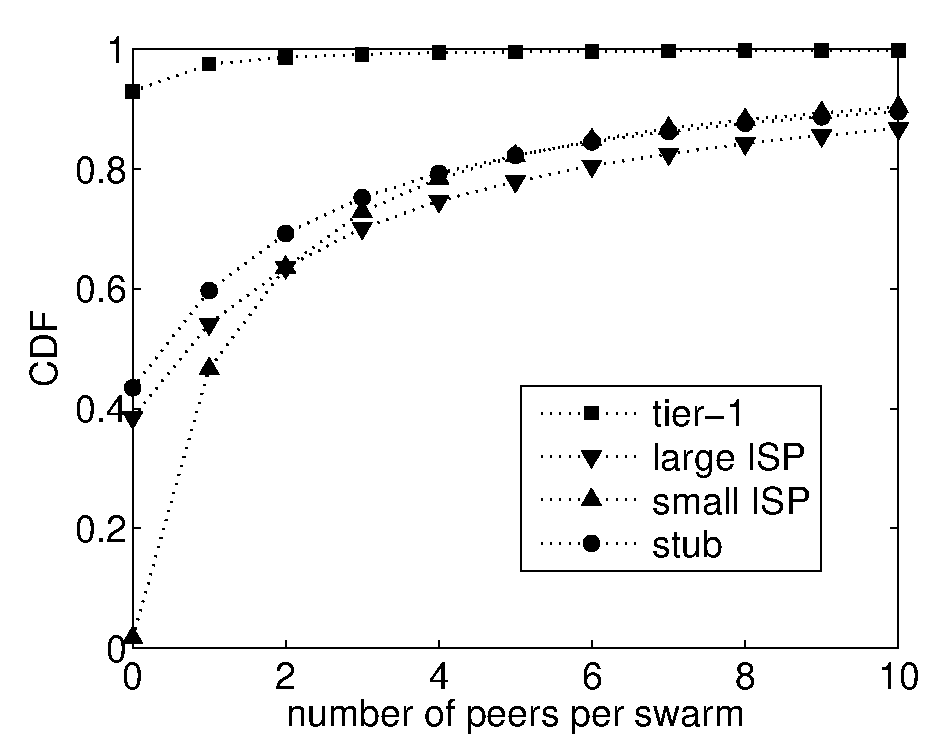
\includegraphics[width=\textwidth]{aslevel/p2p/methodology/figs/CDF_npeers_perswarm}
%  	\caption{CDF of the number of peers per swarm depending on the different ISP classes.}
%  	\label{fig:CDF_npeers_perswarm}
% \end{minipage}
% \hspace{0.01\textwidth}
% \begin{minipage}[b]{0.49\textwidth}
% 	\centering
% 	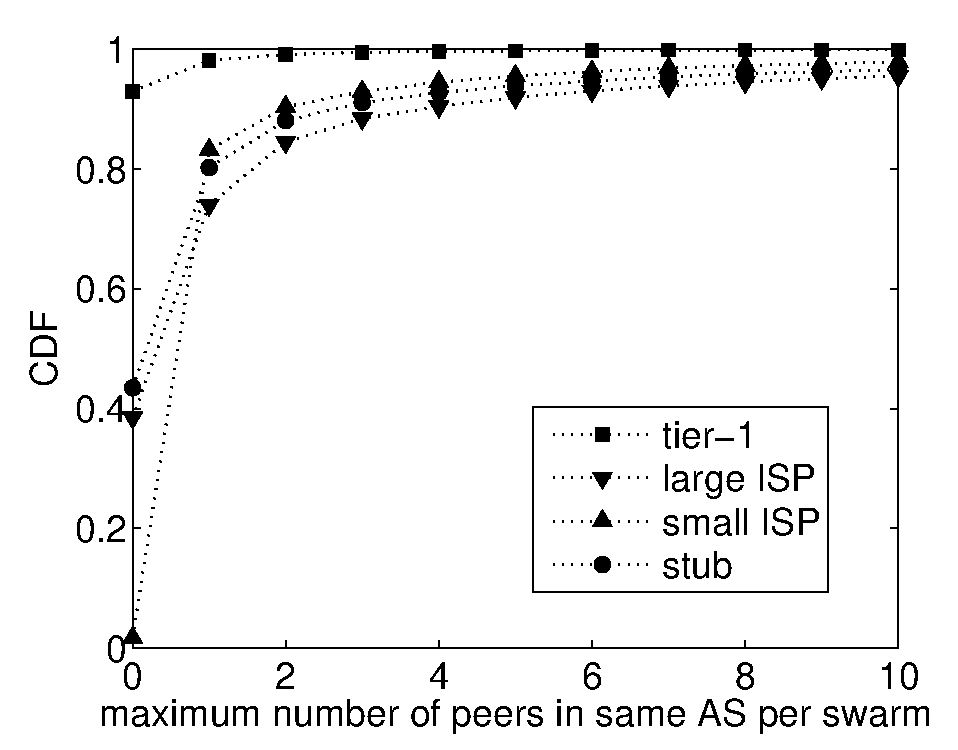
\includegraphics[width=\textwidth]{aslevel/p2p/methodology/figs/CDF_maxpeers_perswarm_perAS}
%  	\caption{CDF of the maximum number of peers in same AS per swarm depending on the tier.}
%  	\label{fig:CDF_maxpeers_perswarm_perAS}
% \end{minipage}
% \end{figure*}

%\begin{figure*}[bt]
%\begin{minipage}[b]{0.32\textwidth}
%	\centering
%	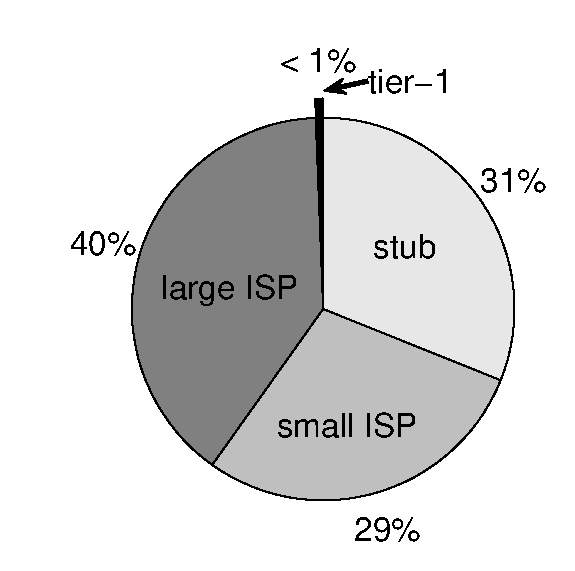
\includegraphics[width=0.8\textwidth]{aslevel/p2p/methodology/figs/npeers_perTier}
% 	\caption{Ratio of peers per ISP class aggregated over all swarms in the measurement set.}
% 	\label{fig:npeers_perTier}
%\end{minipage}
%\hspace{0.01\textwidth}
%\begin{minipage}[b]{0.32\textwidth}
%	\centering
%	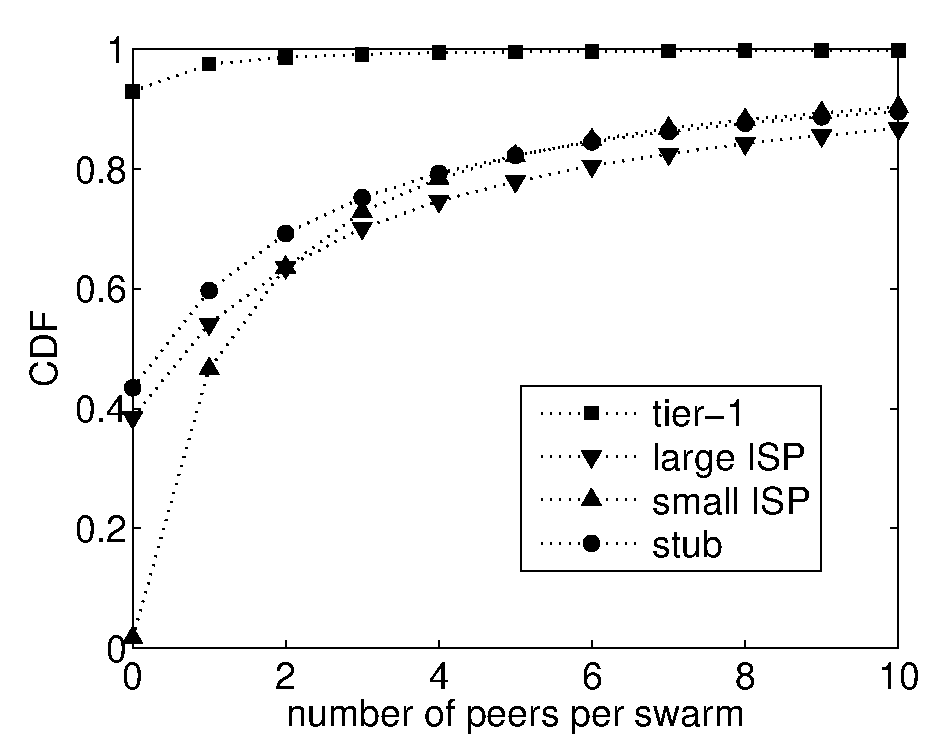
\includegraphics[width=\textwidth]{aslevel/p2p/methodology/figs/CDF_npeers_perswarm}
% 	\caption{CDF of the number of peers per swarm depending on the different ISP classes.}
% 	\label{fig:CDF_npeers_perswarm}
%\end{minipage}
%\hspace{0.01\textwidth}
%\begin{minipage}[b]{0.32\textwidth}
%	\centering
%	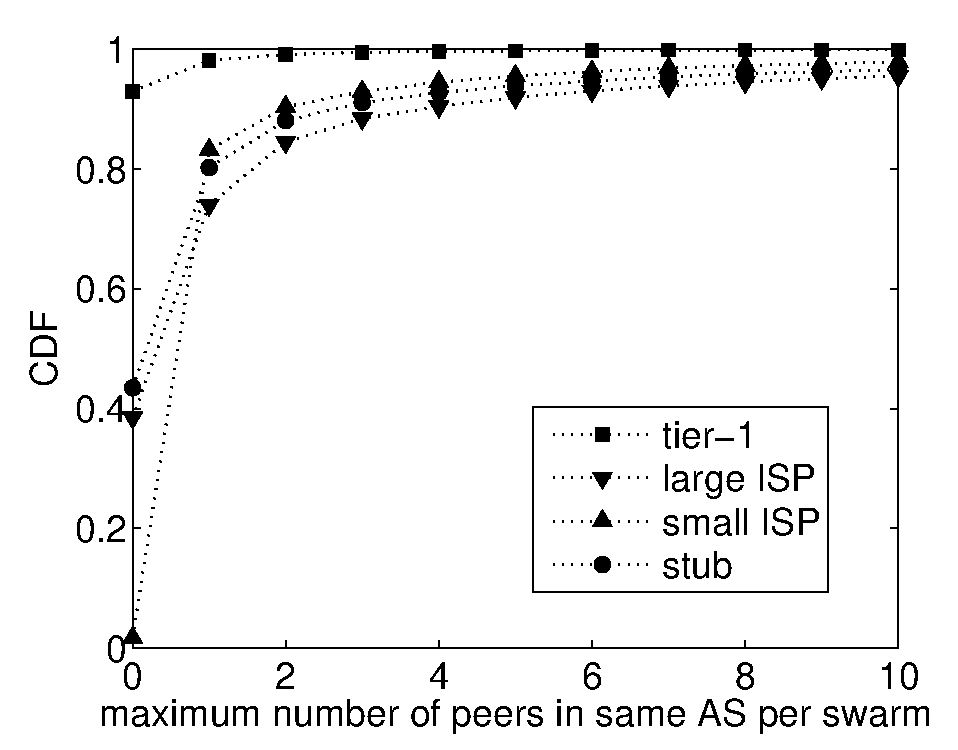
\includegraphics[width=\textwidth]{aslevel/p2p/methodology/figs/CDF_maxpeers_perswarm_perAS}
% 	\caption{CDF of the maximum number of peers in same AS per swarm depending on the tier.}
% 	\label{fig:CDF_maxpeers_perswarm_perAS}
%\end{minipage}
%\end{figure*}

\subsubsection{Cost Model}

To be able to estimate the costs for ASs arising from transit services, we need to know how much traffic is generated and how much providers charge customers for forwarding the traffic.
We consider a snapshot and assume instantaneous traffic rates, i.e., the file-size of the download can be neglected.
For simplicity we make assumptions on how much traffic is generated in each swarm, depending on the the number and location of peers.
\newtheorem{assa}{Assumption}\begin{assa}\label{npeers}
The traffic generated by a peer is equally shared among its neighbors.
\end{assa}
\newtheorem{assb}[assa]{Assumption}\begin{assb}\label{ntraffic}
All peers generate traffic at the same rate.
\end{assb}
\newtheorem{assc}[assa]{Assumption}\begin{assc}\label{npaths}
The traffic between ASs is equally shared among the paths that connect them.
\end{assc}
In practice, traffic rates are allocated by BitTorrent's choke algorithm, which takes into account the upload and download speed of the other peers. Further on, traffic is generally not shared among different AS paths. But, since we consider the aggregated traffic of a large number of swarms, we argue that these assumptions are reasonable and the results do not change significantly.
%and differ for every peer according to its upload bandwidth. Further on,
\paragraph{Traffic Amount}
% We distinguish inter AS traffic and intra AS traffic. Intra-AS traffic is the traffic locally generated by peers which are in the same AS. For intra-AS traffic the AS path has zero AS hops. We estimate the amount of intra-AS traffic proportional to the number of possible directed connections between peers in the source AS. Let $n_{src}$ be the number of peers in the source AS and $\hat n_{src}$ be the number of peers that are in the source AS and in the neighbor set. Then the intra-AS traffic is calculated by
% \begin{equation}
% \frac {\hat n_{\alpha} \cdot (\hat n_{\alpha}-1)} {N} .
% \end{equation}

We use the above assumptions to estimate the traffic generated by the BitTorrent swarms.
Assumption~\ref{npeers} implies, that the traffic sent by a given peer $p_1$ is equally distributed among its $N$ neighbors. Hence, the traffic $p_1$ sends to a neighbor $p_2$ is
\begin{equation}
T(p_1,p_2)=\frac 1 N \, .
\end{equation}
Assumption~\ref{ntraffic} implies that the traffic originating in a given AS $\alpha$ is proportional to the number of peers located in this AS.
Let $\mathcal S$ be the set of all swarms, then the traffic of all swarms that is sent from AS $\alpha$ to AS $\beta$ can be calculated by
\begin{equation}
T(\alpha,\beta)=\sum_{s \in \mathcal S}\sum_{\genfrac{}{}{0pt}{}{\alpha\in s,}{p_1\in\alpha}}\sum_{\genfrac{}{}{0pt}{}{\beta\in s,}{p_2\in\beta}}T(p_1,p_2) \, .
\end{equation}

%Since the traffic is equally distributed among the neighbors, the inter-AS traffic originating from a source AS $src$ is proportional to the number of neighbors $\hat n_{dst}$ in the destination AS $dst$.
The set of AS paths connecting AS $\alpha$ with $\beta$ obtained by the AS inference algorithm is given by $\mathbb P(\alpha,\beta)$.
Assumption~\ref{npaths} implies that the traffic between $\alpha$ and $\beta$ and later the costs are shared equally among the paths in $\mathbb P(\alpha,\beta)$. Hence, we can calculate the traffic on a path $P\in\mathbb P(\alpha,\beta)$.

\begin{equation}
T(P)=\frac 1 {|\mathbb P(\alpha,\beta)|} \cdot T(\alpha,\beta),\;\;\; P\in\mathbb P(\alpha,\beta) \, .
\end{equation}

Next we can calculate the link load $L(\alpha,\beta)$ on the link between two directly connected ASs $\alpha$ and $\beta$. We use $\alpha\leftrightarrow \beta \in P$ as notation for a direct link between $\alpha$ and $\beta$ on the path $P$. The link load is the sum of the load on all paths sharing the link $\alpha\leftrightarrow\beta$.

\begin{equation}\label{equ:linkload}
L(\alpha,\beta)=\sum_{P|\alpha\leftrightarrow \beta \in P} T(P) \, .
\end{equation}

As we consider each AS in a swarm as source AS, the outgoing AS traffic equals the incoming AS traffic. Therefore, we only consider the outgoing AS traffic as inter-AS traffic. The in- and outgoing traffic for AS $\alpha$ is the sum of all loads on links connecting $\alpha$.

\begin{equation}\label{equ:outgoing}
in(\alpha) = out(\alpha) = \sum_{\beta| \exists P, \alpha\leftrightarrow \beta \in P} L(\alpha,\beta) \, .
\end{equation}

In the following we estimate the transit costs. The transit costs are weighted by the link loads defined in this section.
% Hence, we estimate the outgoing traffic $\zeta(p)$ of ASs on paths $p \in \Gamma_{src,dst},$ for $n_{src}$ peers in $src$, and $\hat n_{dst}$ out of $N$ neighbors in $dst$ by

% \begin{equation}
% \zeta(p) = \frac {n_{src} \cdot \hat n_{dst}} {N\cdot |\Gamma_{src,dst}|} .
% \end{equation}

% Hence, in each swarm a total traffic of
% \begin{equation}
% \sum_{src \in \Lambda} \sum_{dst \in \Lambda \backslash \{src\}} \left(\frac {n_{src} \cdot n_{dst}} {N\cdot |\Gamma_{src,dst}|} + \frac {n_{src} \cdot (n_{src}-1)} {N}\right)
% \end{equation}
% is produced. With the set of ASs $\Lambda$.

\subsubsection{Transit Costs}

The business relationships between ISPs define the exact transit costs, but they are part of the private contracts between the ISPs. Hence, we develop a simple model for the arising transit costs. It is common that peering ASs exchange their traffic and the traffic of their customers without charging. Hence, we assume no costs for peering links. The amount a customer pays a provider for transit for a specific volume of traffic is unclear, so we set it to one cost unit, i.e., $1$. That is not the case in practice, but as we have a large number of ASs and swarms, we get a qualitatively good estimation.\\
%For given $\alpha$ and $\beta$ and the set of AS paths $\Gamma_{src,dst}$ we estimate costs, revenues and the balance for every AS occurring on the AS paths connection $src$ and $dst$.
The \textit{costs} of an AS $\alpha$ are increased, if it acts as customer of an AS $\beta$. The costs are increased by one unit weighted by the amount of traffic on the link connecting $\alpha$ and $\beta$, i.e., $L(\alpha, \beta)$ from \refequ{equ:linkload}. Let $\mathcal P(\alpha)$ be the set of providers of $\alpha$, and let $\mathcal C(\alpha)$ be the set of customers of $\alpha$. Then we can calculate the costs of AS $\alpha$ emerging in all swarms as follows.
\begin{equation}\label{equ:costs}
costs(\alpha) = \sum_{\beta\in\mathcal P(\alpha)} L(\alpha,\beta) \, .
\end{equation}
In the same way we can calculate the \textit{revenues} for all AS links and swarms, where $\alpha$ acts as provider.
\begin{equation}\label{equ:revenues}
revenues(\alpha) = \sum_{\beta\in \mathcal C(\alpha)} L(\alpha,\beta) \, .
\end{equation}
The \textit{balance} is the difference between revenues and costs.
\begin{equation}\label{equ:balance}
balance(\alpha) = revenues(\alpha)-costs(\alpha) \, .
\end{equation}

\subsection{Measurement Results}
\label{sec:results}

In this section we show the results of the distributed measurement of the global CDN.
The obtained results show the distribution of clients and servers over different countries.
Furthermore, the mapping on autonomous systems gives insights to the coverage of the Internet.

\subsubsection{Distribution of Vantage Points on Countries}

To investigate the coverage of measurement points we study the distribution of the PlanetLab nodes and Crowdsourcing workers.
Figure~\ref{fig:PLSrc} shows the distribution of PlanetLab nodes on countries over the world.
The pie chart is denoted with the country codes and the percentage of PlanetLab nodes in the respective country.
Most of the 220 clients are located in the US with 15\% of all clients.
However, more than 50\% of the clients are located in West-Europe.
Only few clients are located in different parts of the world.
The tailored distribution towards Western countries is caused by the fact, that the majority of the PlanetLab nodes are located in the US or in western Europe.

\begin{figure}[bt]
    \centering
	\begin{subfigure}[t]{0.49\textwidth}
	\includegraphics[width=\textwidth]{aslevel/crowd/results/figs/PLSrc.pdf}
\caption{PlanetLab}
\label{fig:PLSrc}
\end{subfigure}
\begin{subfigure}[t]{0.49\textwidth}
	\includegraphics[width=\textwidth]{aslevel/crowd/results/figs/MWSrc.pdf}
\caption{Crowdsourcing}
 	\label{fig:MWSrc}
\end{subfigure}
    \caption{Distribution of measurement points on countries in a) PlanetLab and b) Crowdsourcing platform.}
    \label{fig:Src}
\end{figure}

%\begin{figure}[tb]
%	\centering
% 	\includegraphics[width=0.5\textwidth]{figures/Diagramme/Geo/PLSrc.pdf}
%  	\caption{Distribution of PlanetLab nodes over countries.}
%  	\label{fig:PLSrc}
%\end{figure}

Figure~\ref{fig:MWSrc} shows the geo-location of workers on the crowdsourcing platform.
In contrast to PlanetLab, most of the 247 measurement points are located in Asia-Pacific and East-Europe.
The majority of the participating workers 20\% are from Bangladesh followed by Romania and the US with 10\%.
This bias is caused by the overall worker distribution on the platform~\cite{conf2011-410}. However, this can be influences to a certain extend by limiting the access to the tasks to certain geographical regions.
%The payment for crowdsourcing tasks is equal for all countries.
%Hence, the reward is higher for people living in developing countries with less value of money.
%This makes crowdsourcing platforms interesting for people in these countries and leads to a tailored distribution of clients towards different parts of the world.

%\begin{figure}[tb]
%	\centering
% 	\includegraphics[width=0.5\textwidth]{figures/Diagramme/Geo/MWSrc.pdf}
%  	\caption{Distribution of microworkers over countries.}
%  	\label{fig:MWSrc}
%\end{figure}
\subsubsection{Distribution of Identified YouTube Servers on Countries}

To investigate the expansion of the YouTube CDN we study the distribution of YouTube servers over the world.
Figure~\ref{fig:PLDst} shows the location of the servers identified by the PlanetLab nodes.
The requests are mainly directed to servers in the US. Only 20\% of the requests were directed to servers not located in the US.

\begin{figure}[bt]
    \centering
	\begin{subfigure}[t]{0.49\textwidth}
	\includegraphics[width=\textwidth]{aslevel/crowd/results/figs/PLDest.pdf}
  \caption{PlanetLab}
	\label{fig:PLDst}
  \end{subfigure}
	\begin{subfigure}[t]{0.49\textwidth}
	\includegraphics[width=\textwidth]{aslevel/crowd/results/figs/MWDest.pdf}
  \caption{Crowdsourcing}
 	\label{fig:MWDst}
  \end{subfigure}
    \caption{Distribution of physical YouTube servers on countries accessed from a) PlanetLab nodes and b) workers of a crowdsourcing platform.}
    \label{fig:Dst}
\end{figure}

%\begin{figure}[tb]
%	\centering
% 	\includegraphics[width=0.5\textwidth]{figures/Diagramme/Geo/PLDest.pdf}
%  	\caption{Distribution of YouTube servers accessed from PlanetLab nodes.}
%  	\label{fig:PLDst}
%\end{figure}

The servers identified by the crowdsourcing measurement are shown in Figure~\ref{fig:MWDst}.
The amount of requests being directed to servers located in the US is still high.
44\% of clients were directed to the US.
However, in this case the amount of requests resolved to servers outside the US is higher.
In contrast to the PlanetLab measurement many requests are served  locally in the countries of clients.
Furthermore, the decrease of 80\% to 44\% of request being directed to the US shows a huge difference.

%\begin{figure}[tb]
%	\centering
% 	\includegraphics[width=0.5\textwidth]{figures/Diagramme/Geo/MWDest.pdf}
%  	\caption{Distribution of YouTube servers accessed from crowdsourcing users.}
%  	\label{fig:MWDst}
%\end{figure}

Hence, network probes being overrepresented in the US and Europe leads to a limited  view of the content delivery network and the Internet.
This shows the impact of different locations of measurement points on the view of the CDN.
It also demands a careful choice of vantage points for a proper design of experiments in distributed network measurements.
Although both sets of measurement points are globally distributed the fraction of the CDN which is discovered by the probes has very different characteristics.

The amount of servers which is located in the US almost doubles for the PlanetLab measurement.
While 44\% of the requests are resolved to US servers in the Crowdsourcing measurement, nearly all requests of PlanetLab nodes are served by YouTube servers located in the US.
Although less than 15\% of clients are in US, requests are frequently directed to servers in the US. That means that there is still potential to further distribute the content in the CDN.

\subsubsection{Coverage of Autonomous Systems with YouTube Servers}

To identify the distribution of clients on ISPs  and to investigate the expansion of CDNs on autonomous systems we map the measurement points to the corresponding autonomous systems.

%\begin{figure}[tb]
%	\centering
% 	\includegraphics[width=0.5\textwidth]{figures/valli_AS_pl_src.pdf}
%  	\caption{Distribution of PlanetLab nodes over autonomous systems.}
%  	\label{fig:AS_mw_src}
%\end{figure}
%
%\begin{figure}[tb]
%	\centering
% 	\includegraphics[width=0.5\textwidth]{figures/valli_AS_mw_src.pdf}
%  	\caption{Distribution of crowdsourcing clients over autonomous systems.}
%  	\label{fig:AS_mw_src}
%\end{figure}

Figure~\ref{fig:AS_pl_dst} shows the autonomous systems of YouTube servers accessed by PlanetLab nodes.
The autonomous systems were ranked by the number of YouTube servers located in the AS.
The empirical probability $P(k)$ that a server belongs to AS with rank $k$ is depicted against the AS rank.
The number of autonomous systems hosting YouTube servers that are accessed by PlanetLab nodes is limited to less than 30.
The top three ranked ASs are AS15169, AS36040 and AS43515.
AS15169 is the Google autonomous system which includes the Google backbone.
The Google backbone is a global network that reaches to worldwide points of presence to offer peering agreements at peering points.
AS36040 is the YouTube network connecting the main datacenter in Mountain-View which is also managed by Google.
AS43515 belongs to the YouTube site in Europe which is administrated in Ireland.
Hence, two thirds of the servers are located in an autonomous systems which is managed by Google.
Only few requests are served from datacenters not being located in a Google AS.
The reason that request from PlanetLab are most frequently served by ASs owned by Google might be a good interconnection of the NRENs to the Google ASs.

\begin{figure}[bt]
    \centering
	\begin{subfigure}[t]{0.49\textwidth}
	\includegraphics[width=\textwidth]{aslevel/crowd/results/figs/valli_AS_pl_dst.pdf}
  \caption{PlanetLab}
	\label{fig:AS_pl_dst}
  \end{subfigure}
	\begin{subfigure}[t]{0.49\textwidth}
	\includegraphics[width=\textwidth]{aslevel/crowd/results/figs/valli_AS_mw_dst.pdf}
  \caption{Crowdsourcing}
 	\label{fig:AS_mw_dst}
  \end{subfigure}
    \caption{Distribution of YouTube servers on autonomous systems from a) PlanetLab and b) Crowdsourcing perspective.}
    \label{fig:AS_dst}
\end{figure}

%\begin{figure}[tb]
%	\centering
% 	\includegraphics[width=0.5\textwidth]{figures/valli_AS_pl_dst.pdf}
%  	\caption{Distribution of YouTube servers over autonomous systems from PlanetLab perspective.}
%  	\label{fig:AS_pl_src}
%\end{figure}

Figure~\ref{fig:AS_mw_dst} depicts the autonomous systems where requests to YouTube videos from  the crowdsourcing workers were directed.
The empirical probability that a server belongs to an AS has been plotted dependent on the AS rank.
The YouTube servers identified by the crowdsourcing probes are located in more than 60 autonomous systems.
Hence, the YouTube CDN is expanded on a higher range of ASs from the crowdsourcing perspective compared to PlanetLab.
Again the three autonomous systems serving most requests are the ASs managed by Google, respectively YouTube.
But the total number of requests served by a Google managed AS is only 41\%.
Hence, in contrary to the PlanetLab measurement, requests are served most frequently from ASs not owned by Google.
Here, caches at local ISPs  managed by YouTube could be used to bring the content close to users without providing own infrastructure.
This would also explain the large number of identified ASs providing a YouTube server.
The results show that the PlanetLab platform is not capable to measure the structure of a global CDN, since large parts of the CDN are not accessed by clients in NRENs.
%The aim of this work was to compare the measurement capabilities of the concurring platforms, opposed to a complete measurement of the YouTube CDN.
%It is part of future work to perform an exhaustive measurement study based on PlanetLab and crowdsourcing platforms, which produces a representative view from gobally distributed vantage points on the YouTube CDN and its distribution on autonomous systems.

%Crowdsourcing identifies a higher range of different ASs

%\begin{figure}[tb]
%	\centering
% 	\includegraphics[width=0.5\textwidth]{figures/valli_AS_mw_dst.pdf}
%  	\caption{Distribution of YouTube servers over autonomous systems from crowdsourcing end-user perspective.}
%  	\label{fig:AS_mw_src}
%\end{figure}

%TODO identify overlaps.

%A substantial number of servers is not located in a Google AS
%Heterogeneous distribution. Implication on measurement. Optimize measurement framework?


\section{Content Delivery Network Characterization by Distributed Active Measurements}\label{sec:aslevel:crowd}

%The most popular peer-to-peer overlay network today is BitTorrent.
%Therefore we focus on BitTorrent.
% motivation
%Internet video constitutes more than half of all consumer Internet traffic globally, and its percentage will further increase \cite{ciscovni2013}. Most of the video traffic is delivered by content delivery networks (CDNs). Today the world's largest video CDN is YouTube. Since Google took over YouTube in 2006 the infrastructure of the video delivery platform has grown to be a global content delivery network.
%The global expansion of the CDN was also necessary to cope with growing demand of user demands and the high expectations on the video playback. Therefore, content delivery networks try to bring content geographically close to users.
%However, the traffic from content delivery networks is highly asymmetric and produces a large amount of costly inter-domain traffic \cite{labovitz2010internet}. Especially Internet Service Providers~(ISPs) providing access to many end users have problems to deal with the huge amount of traffic originating from YouTube. Furthermore, the Google CDN is constantly growing and changing, which makes it difficult for access providers to adapt their infrastructure accordingly.

% problem statement
To understand and monitor the impact of YouTube traffic on ISPs and the topology of CDNs appropriate measurements are acquired. Due to YouTube's load-balancing and caching mechanisms the YouTube video server selection is highly dependent on the location of the measurement points. Hence, we need a globally distributed measurement platform to perform active measurements to uncover the location of YouTube servers.
%Recent work \cite{adhikari2012vivisecting,adhikari2011you} has performed such measurements in PlanetLab~\cite{planetlab}, a global test bed that provides measurement nodes at universities and research institutes.
The problem is that probes disseminated from PlanetLab nodes origin solely from National Research and Education Networks~(NRENs). This may not reflect the perspective of access ISPs which have a different connection to the YouTube CDN with different peering or transit agreements.
% our methodology
To achieve a better view on the YouTube CDN from the perspective of end users in access networks we use a commercial crowdsourcing platform to recruit regular Internet users as measurement probes.
This complementary view can help to gain a better understanding of the characteristics of Video CDNs.
%Thus, we increase the coverage of vantage points for the distributed measurement of the YouTube CDN.
To evaluate the impact of the measurement platform and the coverage of their vantage point,  we perform the same measurements using PlanetLab nodes and crowdsourcing users and compare the obtained results.

% our contribution
%Our measurements show that distributed measurements in PlanetLab are not capable to capture a globally distributed network, since the PlanetLab nodes are located in NRENs where the view on the Internet is limited. We demonstrate that recruiting users via crowdsourcing platforms as measurement probes can offer a complementary view on the Internet, since they provide access to real end users devices located out side of these dedicated research networks.
%Concepts like ALTO or economic traffic management (ETM) \cite{hossfialong} need a global view of the CDN structure to optimize traffic beyond the borders of ISPs.
%what in turn  might have implications for network operators in mechanism design and resource provisioning.
%Finally, models for simulation and performance evaluation of mechanisms incorporating CDNs need to apply the characteristics identified by crowd sourced network measurements.
%In this work, we propose a new measurement methodology which benefits of the distribution of crowdsourcing workers on internet access provider networks.

% structure
The measurements conducted in the PlanetLab and via crowdsourcing are described in Section~\ref{sec:crowd:method}.
In Section~\ref{sec:crowd:results} we provide details on the measurement results and their importance for the design of distributed network measurements.

%\input{aslevel/crowd/crowdsourcing/crowdsourcing}
\subsection{Distributed Active Measurement Setup}
\label{sec:crowd:method}

To assess the capability of crowdsourcing for distributed active measurements we conduct measurements with both  PlanetLab and the commercial Crowdsourcing platform Microworkers~\cite{microworkers}.
We measure the global expansion of the YouTube CDN by resolving physical server IP-addresses for clients in different locations.

\subsubsection{Description of the PlanetLab Measurement}

PlanetLab is a publicly available test bed, which currently consists of 1173 nodes at 561 sites.
The sites are usually located at universities or research institutes.
Hence, they are connected to the Internet via NRENs.
To conduct a measurement in PlanetLab a slice has to be set up which consists of a set of virtual machines running on different nodes in the PlanetLab test bed.
Researchers can then access these slides to install measurement scripts.
In our case the measurement script implemented in Java extracted the server hostnames of the page of three predetermined YouTube videos and resolved the IP addresses of the physical video servers.
The IP addresses of the PlanetLab clients and the resolved IP addresses of the physical video servers were stored in a database.
To be able to investigate locality in the YouTube CDN, the geo-location of servers and clients is necessary.
For that purpose the IP addresses were mapped to geographic coordinates with MaxMinds GeoIP database \cite{geolite}.
The measurement was conducted on 220 randomly chosen PlanetLab nodes in March 2012.

\subsubsection{Description of the Crowdsourcing Measurement}
To measure the topology of the YouTube CDN from an end users point of view who is connected by an ISP network we used the crowdsourcing platform Microworker~\cite{microworkers}.
The workers were asked to access a web page with an embedded Java application, which automatically conducts client side measurements.
These include, among others, the extraction of the default and fallback server URLs from three predetermined YouTube video pages.
The extracted URLs were resolved to the physical IP address of the video servers locally on the clients.
The IP addresses of video servers and of the workers client were sent to a server which collected all measurements and stored them in a database.

In a first measurement run, in December 2011, 60 different users of Microworkers participated in the measurements.
Previous evaluation have shown, that the majority of the platform users is located in Asia~\cite{conf2011-410}, and accordingly most of the participants of there first campaign were from Bangladesh.
In order to obtain wide measurement coverage the number of Asian workers participating in a second measurement campaign, conducted in March 2012, was restricted.
In total, 247 workers from 32 different countries, finished the measurements successfully identifying 1592 unique physical YouTube server IP addresses.

\subsection{Measurement Results and Their Implications}
\label{sec:crowd:results}

In this section we show the results of the distributed measurement of the global CDN.
The obtained results show the distribution of clients and servers over different countries.
Furthermore, the mapping on autonomous systems gives insights to the coverage of the Internet.

\subsubsection{Distribution of Vantage Points on Countries}

To investigate the coverage of measurement points we study the distribution of the PlanetLab nodes and Crowdsourcing workers.
Figure~\ref{fig:PLSrc} shows the distribution of PlanetLab nodes on countries over the world.
The pie chart is denoted with the country codes and the percentage of PlanetLab nodes in the respective country.
Most of the 220 clients are located in the US with 15\% of all clients.
However, more than 50\% of the clients are located in West-Europe.
Only few clients are located in different parts of the world.
The tailored distribution towards Western countries is caused by the fact, that the majority of the PlanetLab nodes are located in the US or in western Europe.

\begin{figure}[bt]
    \centering
	\begin{subfigure}[t]{0.49\textwidth}
	\includegraphics[width=\textwidth]{aslevel/crowd/figs/PLSrc.pdf}
\caption{PlanetLab}
\label{fig:PLSrc}
\end{subfigure}
\begin{subfigure}[t]{0.49\textwidth}
	\includegraphics[width=\textwidth]{aslevel/crowd/figs/MWSrc.pdf}
\caption{Crowdsourcing}
 	\label{fig:MWSrc}
\end{subfigure}
    \caption{Distribution of measurement points on countries in a) PlanetLab and b) Crowdsourcing platform.}
    \label{fig:Src}
\end{figure}

%\begin{figure}[tb]
%	\centering
% 	\includegraphics[width=0.5\textwidth]{figures/Diagramme/Geo/PLSrc.pdf}
%  	\caption{Distribution of PlanetLab nodes over countries.}
%  	\label{fig:PLSrc}
%\end{figure}

Figure~\ref{fig:MWSrc} shows the geo-location of workers on the crowdsourcing platform.
In contrast to PlanetLab, most of the 247 measurement points are located in Asia-Pacific and East-Europe.
The majority of the participating workers 20\% are from Bangladesh followed by Romania and the US with 10\%.
This bias is caused by the overall worker distribution on the platform~\cite{conf2011-410}. However, this can be influences to a certain extend by limiting the access to the tasks to certain geographical regions.
%The payment for crowdsourcing tasks is equal for all countries.
%Hence, the reward is higher for people living in developing countries with less value of money.
%This makes crowdsourcing platforms interesting for people in these countries and leads to a tailored distribution of clients towards different parts of the world.

%\begin{figure}[tb]
%	\centering
% 	\includegraphics[width=0.5\textwidth]{figures/Diagramme/Geo/MWSrc.pdf}
%  	\caption{Distribution of microworkers over countries.}
%  	\label{fig:MWSrc}
%\end{figure}
\subsubsection{Distribution of Identified YouTube Servers on Countries}

To investigate the expansion of the YouTube CDN we study the distribution of YouTube servers over the world.
Figure~\ref{fig:PLDst} shows the location of the servers identified by the PlanetLab nodes.
The requests are mainly directed to servers in the US. Only 20\% of the requests were directed to servers not located in the US.

\begin{figure}[bt]
    \centering
	\begin{subfigure}[t]{0.49\textwidth}
	\includegraphics[width=\textwidth]{aslevel/crowd/figs/PLDest.pdf}
  \caption{PlanetLab}
	\label{fig:PLDst}
  \end{subfigure}
	\begin{subfigure}[t]{0.49\textwidth}
	\includegraphics[width=\textwidth]{aslevel/crowd/figs/MWDest.pdf}
  \caption{Crowdsourcing}
 	\label{fig:MWDst}
  \end{subfigure}
    \caption{Distribution of physical YouTube servers on countries accessed from a) PlanetLab nodes and b) workers of a crowdsourcing platform.}
    \label{fig:Dst}
\end{figure}

%\begin{figure}[tb]
%	\centering
% 	\includegraphics[width=0.5\textwidth]{figures/Diagramme/Geo/PLDest.pdf}
%  	\caption{Distribution of YouTube servers accessed from PlanetLab nodes.}
%  	\label{fig:PLDst}
%\end{figure}

The servers identified by the crowdsourcing measurement are shown in Figure~\ref{fig:MWDst}.
The amount of requests being directed to servers located in the US is still high.
44\% of clients were directed to the US.
However, in this case the amount of requests resolved to servers outside the US is higher.
In contrast to the PlanetLab measurement many requests are served  locally in the countries of clients.
Furthermore, the decrease of 80\% to 44\% of request being directed to the US shows a huge difference.

%\begin{figure}[tb]
%	\centering
% 	\includegraphics[width=0.5\textwidth]{figures/Diagramme/Geo/MWDest.pdf}
%  	\caption{Distribution of YouTube servers accessed from crowdsourcing users.}
%  	\label{fig:MWDst}
%\end{figure}

Hence, network probes being overrepresented in the US and Europe leads to a limited  view of the content delivery network and the Internet.
This shows the impact of different locations of measurement points on the view of the CDN.
It also demands a careful choice of vantage points for a proper design of experiments in distributed network measurements.
Although both sets of measurement points are globally distributed the fraction of the CDN which is discovered by the probes has very different characteristics.

The amount of servers which is located in the US almost doubles for the PlanetLab measurement.
While 44\% of the requests are resolved to US servers in the Crowdsourcing measurement, nearly all requests of PlanetLab nodes are served by YouTube servers located in the US.
Although less than 15\% of clients are in US, requests are frequently directed to servers in the US. That means that there is still potential to further distribute the content in the CDN.

\subsubsection{Coverage of Autonomous Systems with YouTube Servers}

To identify the distribution of clients on ISPs  and to investigate the expansion of CDNs on autonomous systems we map the measurement points to the corresponding autonomous systems.

%\begin{figure}[tb]
%	\centering
% 	\includegraphics[width=0.5\textwidth]{figures/valli_AS_pl_src.pdf}
%  	\caption{Distribution of PlanetLab nodes over autonomous systems.}
%  	\label{fig:AS_mw_src}
%\end{figure}
%
%\begin{figure}[tb]
%	\centering
% 	\includegraphics[width=0.5\textwidth]{figures/valli_AS_mw_src.pdf}
%  	\caption{Distribution of crowdsourcing clients over autonomous systems.}
%  	\label{fig:AS_mw_src}
%\end{figure}

Figure~\ref{fig:AS_pl_dst} shows the autonomous systems of YouTube servers accessed by PlanetLab nodes.
The autonomous systems were ranked by the number of YouTube servers located in the AS.
The empirical probability $P(k)$ that a server belongs to AS with rank $k$ is depicted against the AS rank.
The number of autonomous systems hosting YouTube servers that are accessed by PlanetLab nodes is limited to less than 30.
The top three ranked ASs are AS15169, AS36040 and AS43515.
AS15169 is the Google autonomous system which includes the Google backbone.
The Google backbone is a global network that reaches to worldwide points of presence to offer peering agreements at peering points.
AS36040 is the YouTube network connecting the main datacenter in Mountain-View which is also managed by Google.
AS43515 belongs to the YouTube site in Europe which is administrated in Ireland.
Hence, two thirds of the servers are located in an autonomous systems which is managed by Google.
Only few requests are served from datacenters not being located in a Google AS.
The reason that request from PlanetLab are most frequently served by ASs owned by Google might be a good interconnection of the NRENs to the Google ASs.

\begin{figure}[bt]
    \centering
	\begin{subfigure}[t]{0.49\textwidth}
	\includegraphics[width=\textwidth]{aslevel/crowd/figs/valli_AS_pl_dst.pdf}
  \caption{PlanetLab}
	\label{fig:AS_pl_dst}
  \end{subfigure}
	\begin{subfigure}[t]{0.49\textwidth}
	\includegraphics[width=\textwidth]{aslevel/crowd/figs/valli_AS_mw_dst.pdf}
  \caption{Crowdsourcing}
 	\label{fig:AS_mw_dst}
  \end{subfigure}
    \caption{Distribution of YouTube servers on autonomous systems from a) PlanetLab and b) Crowdsourcing perspective.}
    \label{fig:AS_dst}
\end{figure}

%\begin{figure}[tb]
%	\centering
% 	\includegraphics[width=0.5\textwidth]{figures/valli_AS_pl_dst.pdf}
%  	\caption{Distribution of YouTube servers over autonomous systems from PlanetLab perspective.}
%  	\label{fig:AS_pl_src}
%\end{figure}

Figure~\ref{fig:AS_mw_dst} depicts the autonomous systems where requests to YouTube videos from  the crowdsourcing workers were directed.
The empirical probability that a server belongs to an AS has been plotted dependent on the AS rank.
The YouTube servers identified by the crowdsourcing probes are located in more than 60 autonomous systems.
Hence, the YouTube CDN is expanded on a higher range of ASs from the crowdsourcing perspective compared to PlanetLab.
Again the three autonomous systems serving most requests are the ASs managed by Google, respectively YouTube.
But the total number of requests served by a Google managed AS is only 41\%.
Hence, in contrary to the PlanetLab measurement, requests are served most frequently from ASs not owned by Google.
Here, caches at local ISPs  managed by YouTube could be used to bring the content close to users without providing own infrastructure.
This would also explain the large number of identified ASs providing a YouTube server.
The results show that the PlanetLab platform is not capable to measure the structure of a global CDN, since large parts of the CDN are not accessed by clients in NRENs.
%The aim of this work was to compare the measurement capabilities of the concurring platforms, opposed to a complete measurement of the YouTube CDN.
%It is part of future work to perform an exhaustive measurement study based on PlanetLab and crowdsourcing platforms, which produces a representative view from gobally distributed vantage points on the YouTube CDN and its distribution on autonomous systems.

%Crowdsourcing identifies a higher range of different ASs

%\begin{figure}[tb]
%	\centering
% 	\includegraphics[width=0.5\textwidth]{figures/valli_AS_mw_dst.pdf}
%  	\caption{Distribution of YouTube servers over autonomous systems from crowdsourcing end-user perspective.}
%  	\label{fig:AS_mw_src}
%\end{figure}

%TODO identify overlaps.

%A substantial number of servers is not located in a Google AS
%Heterogeneous distribution. Implication on measurement. Optimize measurement framework?

\section{Statistical Characterization of the Distribution of IP Addresses on Autonomous Systems}\label{sec:aslevel:census}

The performance of systems using CPE or resources provided by end-users depend on the capacity and number of devices available.
To assess the potential of a hierarchical cache system in an ISPs network, the number of active subscribers in an autonomous systems has to be known.
Assuming that the number of active IP-addresses is correlated to the number of subscribers in an autonomous system, we use the Internet Census Dataset to determine the distribution of active IP-addresses on autonomous systems.

We use the Internet Census Dataset \cite{carna2013} to determine the number of active IP-addresses for each AS in the Internet.
The Internet Census Dataset provides a scan on the active IP addresses in the Internet based on a full probing of the entire IPv4 Internet.
%The Internet Census Dataset\cite{carna2013} was conducted from June to October 2012.
The scan was conducted from June to October 2012 by infecting several hundred thousand unprotected devices on the Internet to form the so called \emph{carna} botnet.
The botnet functioned as distributed port scanner that transfered the results to a central server.

%The complete IPv4-address room was scanned using a bot-net consisting of 4,200,000 nodes.
In the ICMP ping scan more than 420 million replied to requests more than once.
The service probe data reveal open ports on devices which is used to infer the type of device.
The Internet Census Dataset was validated forensically in \cite{dainotticaida} by aligning the probes of the botnet with the traffic captured at the UCSD Network Telescope \cite{ucsdtelescope}, which is a large darknet, i.e., IP addresses that are inactive, thus not accepting connections.
The raw logs of the carna botnet erroneously reported that a large number of IPs in the darknet were active, likely due to the presence of HTTP proxies.
However, according to \cite{dainotticaida}, only about 3\% of the host probe and port scan logs are potentially affected by this problem.
Unaffected by this issue are the logs based on ICMP pings and actual responses from the target hosts, which are used in our study.
In \cite{krenc2014internet} the scope of the dataset is taken into perspective and show that, although there are some qualitative problems, the measurement data seems to be authentic.
%We use the Internet Census Dataset to determine the number of active IP-addresses for each autonomous system in the Internet.

We use an IP to ASN mapping to derive the autonomous system number for each IP-address. There are different services, that provide an IP to ASN mapping.
The whois-service can be used to get the current ASN for an IP-address.
To enable an efficient evaluation we used the MAXMIND GeoLite ASN database \cite{geo_ip}, which is updated every month and can be downloaded and used as a local database.
The results of the MAXMIND GeoLite ASN database were cross checked with results obtained from whois, which showed no differences.

The ICMP ping scan discovered a total of 598,180,914 IP-addresses.
The service probe scan discovered 244,000 IP-addresses that listen to port 9100 and are identified as print servers, and 70.84 million IP-addresses of web-servers that listen to port 80.
Assuming that most network functions do not reply to ICMP ping requests and neglecting different network functions, this results in 88.1\% of IP-addresses assigned to end-user devices.
Since the Internet Census the number of Internet users increased, which also has to be considered.
According to \cite{itu2015facts} there is a 7\% annual increase in fixed-broadband subscriptions in the past three years.
%From 2012 to 2014 the number of Internet users increased by almost 500,000,000 according to \cite{•}.

% \begin{figure}[tb]
% \centering
% 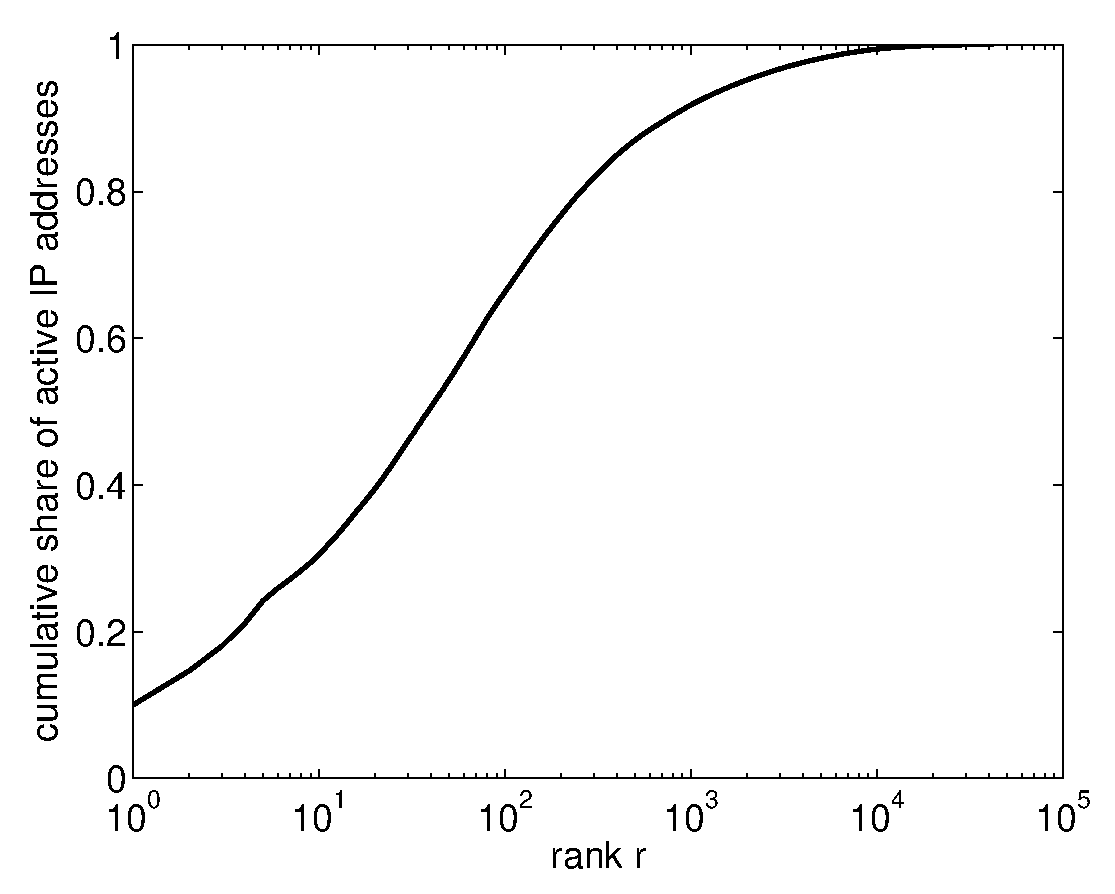
\includegraphics[width=0.49\textwidth]{aslevel/census/figs/shareactiveIPs}
% \caption{Cumulative share of active IP-addresses in autonmous systems ranked in descending order.}
% \label{fig:shareactiveIPs}
% \end{figure}
%
% \begin{figure}[tb]
% \centering
% 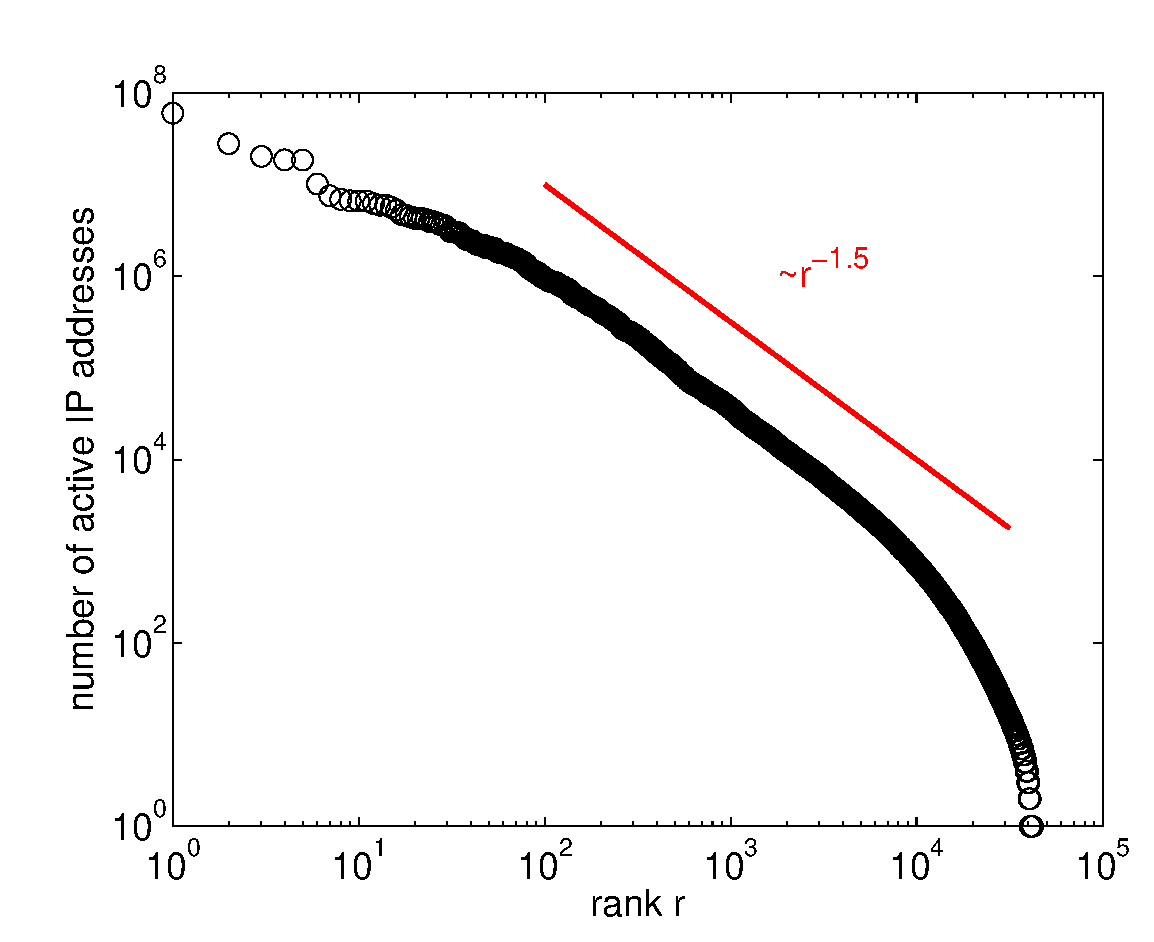
\includegraphics[width=0.49\textwidth]{aslevel/census/figs/activeIPs}
% \caption{Rank of Internet providers with number of active IP-addresses per AS.}
% \label{fig:asrank}
% \end{figure}

\begin{figure*}[bt]
\begin{minipage}[b]{0.49\textwidth}
  \centering
  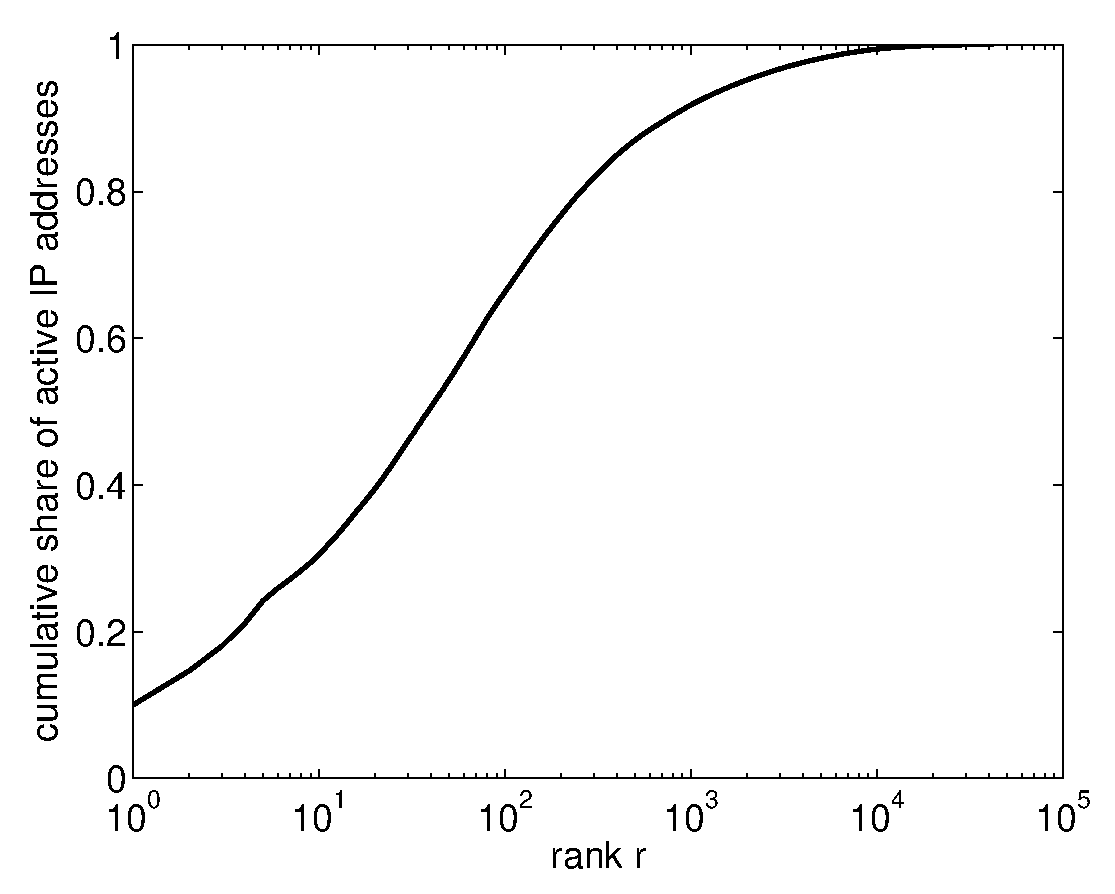
\includegraphics[width=1\textwidth]{aslevel/census/figs/shareactiveIPs}
  \caption{Cumulative share of active IPs in autonmous systems ranked in descending order.}
  \label{fig:shareactiveIPs}
\end{minipage}
\hspace{0.01\textwidth}
\begin{minipage}[b]{0.49\textwidth}
  \centering
  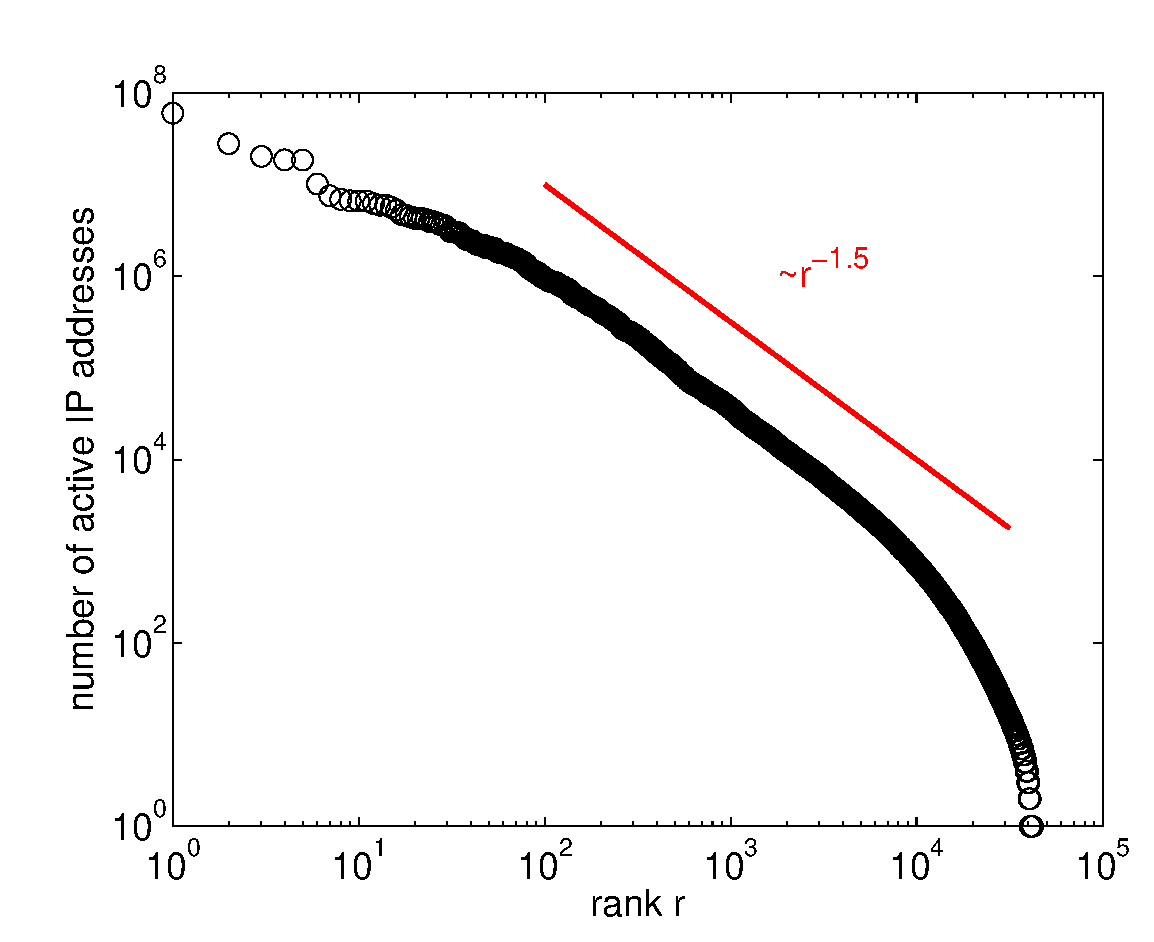
\includegraphics[width=\textwidth]{aslevel/census/figs/activeIPs}
  \caption{Rank of Internet providers with number of active IPs per AS.}
  \label{fig:asrank}
\end{minipage}
\end{figure*}

\reffig{fig:shareactiveIPs} shows the cumulative share of active IP-addresses in the autonomous systems ranked in descending order.
The 100 largest autonomous systems make up 2/3 of active IPs and more than 85\% of the IPs are active in only 1\% of the autonomous systems. The 10 largest autonomous systems already contain 30\% of the active IPs.

\reffig{fig:asrank} shows the number of active IP-addresses per AS ranked in descending order.
The top 5 ASs are shown in table~\ref{tab:asrank}.
The AS with most active IP-addresses is ChinaTelecom with almost 60 million active IPs, followed by another Chinese provider.
The largest AS in the US is Comcast on rank three.
The largest Korean and German providers are ranked 4 and 5 with more than 18 million active IPs.
The number of active IP addresses can be approximated with a power law with slope 1.5 that drops a little for low ranks.
This shows that the distribution of active IP addresses on ASs is highly heterogeneous.
That means the potential of approaches leveraging spare resources on home routers depends on the AS.

\begin{table}[tb]
\centering
\caption{Rank of top 5 provider with most active IP-addresses.}
\label{tab:asrank}
\begin{tabular}{|c|c|c|c|}
\hline
rank r & ASN & provider & \# active IPs  \\
\hline
1 & 4134 & ChinaTelecom & 59,824,824 \\
2 & 4837 & China-Network-Communication-Group & 27,776,643 \\
3 & 7922 & Comcast & 20,227,918 \\
4 & 4766 & KoreaTelecom & 18,502,963 \\
5 & 3320 & DeutscheTelekomAG & 18,476,519 \\
\hline
\end{tabular}
\end{table}
%

%\input{aslevel/census/dataset/dataset}
%\subsection{Numerical Examples and Impact on Transit Costs}\label{sec:hierarchical:simulative:evaluation}

To evaluate the performance of a CDN supported by home routers, two scenarios are simulated. The first scenario simulates requests to a CDN with caches organized in a tree structure and compares isolated caches to cooperating caches to assess the benefit of the overlay.
The second scenario adds an AS topology with peering and transit links to evaluate the inter-domain traffic saving potential.
As described in \refchap{chap:aslevel}, a transit link exists between a customer ISP and its transit provider, if the customer ISP pays the transit provider to forward its traffic destined to parts of the Internet that the customer ISP does not own or cannot reach.

%\subsection{Caching}
% To assess the impact of the number of shared home routers and the size of the ISP, a tiered caching architecture with resource locations at three different tiers, including the main data center of the content provider, CDN caches, and end-user equipment is evaluated.
% The number of different content items to be downloaded or streamed from the resources is specified by the catalog size $N$. Tier-3 resource is the data center of the content provider, where all $N$ content items are stored. Tier-2 resources are edge caches and ISP caches, typically organized in a CDN, which are located close to Internet exchange points or within ISP networks. Requests served by ISPs or edge caches produce less or no inter-domain costs. Thus, these caches are referred as ISP caches in the following. The capacity of ISP caches is given as a fraction of $N$ and is specified by $C_\text{ISP}$. The caching strategy of ISP caches is LRU.
%Each autonomous system hosts an ISP cache.
Within tier-1, the caches are placed on shared home routers. These caches are referred to in the following as home routers (HRs). The cache capacity of HRs is specified by $C_1$ and their caching strategy is LRU. In this study $C_1$ is set to four (4) content items.
We evaluate the performance dependent on the autonomous system size $n_\text{user}$, in terms of the number of end-users in the autonomous system. The probability that an end-user enables the HR to shares contents is given by $p_\text{share}$. The probability that a user requests certain content items depends on the content's popularity distribution, which is specified by the Zipf exponent $\alpha$.

\subsubsection{Benefits of an Overlay}

To evaluate the performance of the overlay, two cases are considered (a) the tree case and (b) the overlay case. In the tree case (a), each user is assigned to one shared HR in its AS. If a user shares its HR, it is assigned only to its HR. A requested item is looked up in the assigned HR initially, i.e. in the tier-3 cache. If the requested item is not found, the request is forwarded to the next tier. The hierarchical caching strategy is leave-copy-everywhere, which means that the video is cached in each cache on the look up path. In the overlay case (b), a requested item is looked up in the HR of the user, if it is not found, it is looked up in shared HRs in the same autonomous system using the overlay. If no tier-3 cache in the AS contains the item it is looked up in tier-2 caches and finally in the data center of the content provider. The hierarchical caching strategy is leave-copy-everywhere, too, with the constraint, that the item is cached in the tier-3 cache only, which was looked up first.

\begin{figure}[tb]
  \centering
  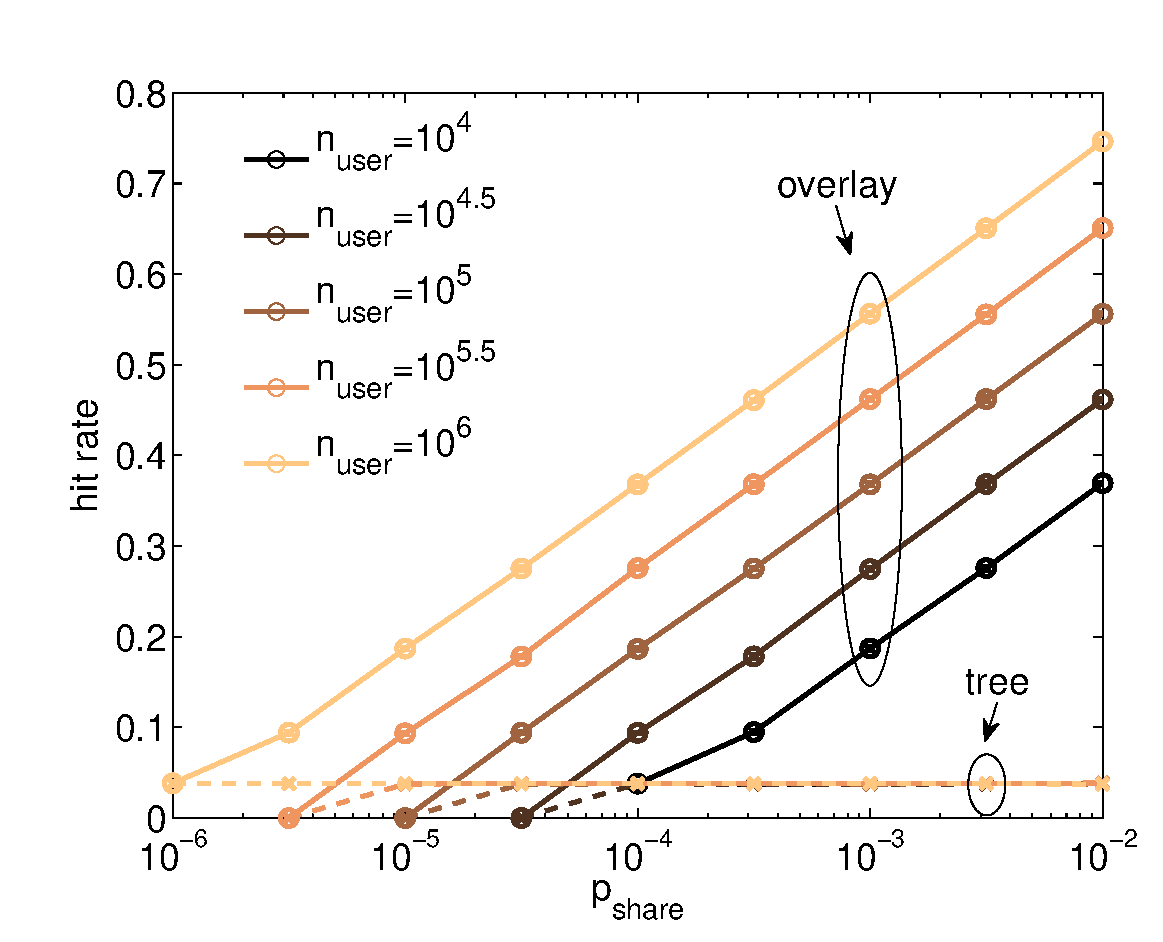
\includegraphics[width=0.7\textwidth]{hierarchical/simulative/figures/overlay_nuser_hitrate3}
  \caption{Hit rate of the overlay dependent on home router sharing probability.}
  \label{fig:overlay_nuser_hitrate}
\end{figure}

\begin{figure}[tb]
  \centering
  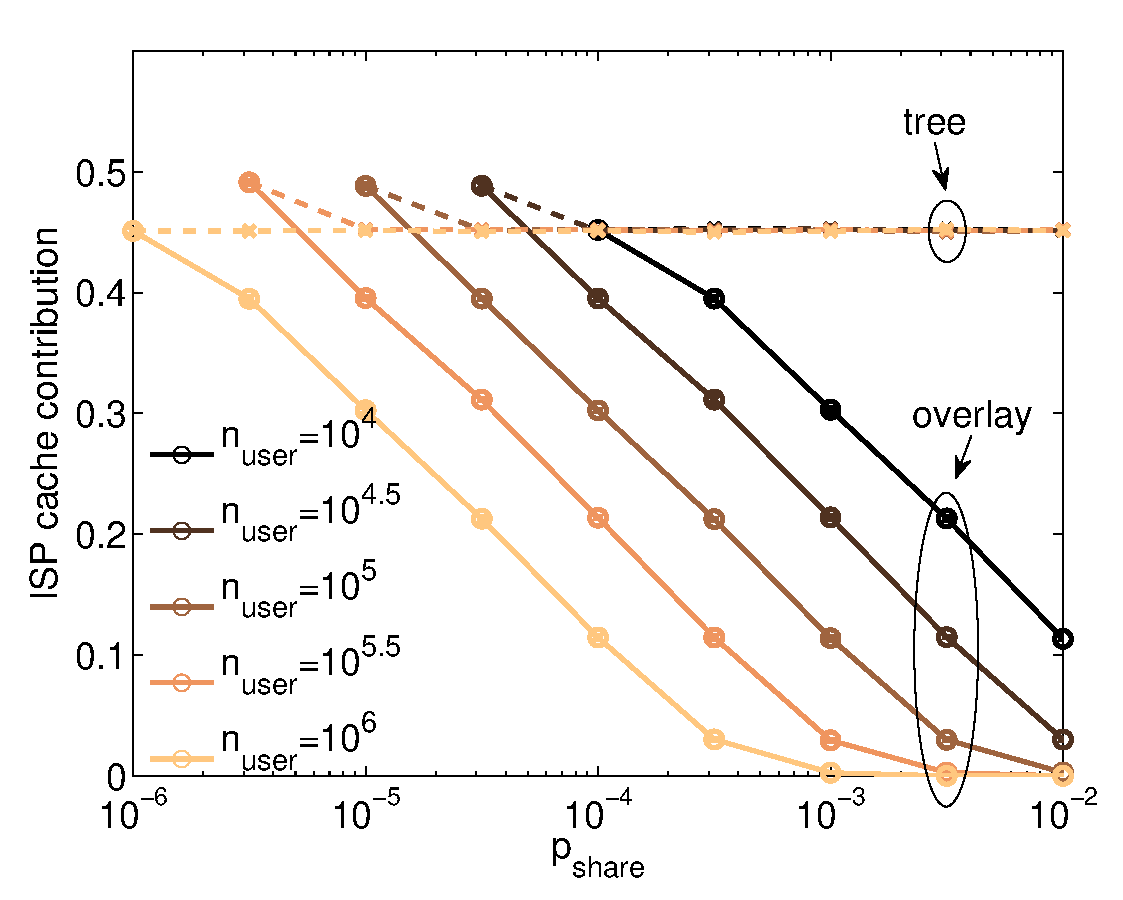
\includegraphics[width=0.7\textwidth]{hierarchical/simulative/figures/overlay_nuser_ISPcontrib3}
  \caption{ISP cache contribution dependent on home router sharing probability.}
  \label{fig:overlay_nuser_ISPcontrib}
\end{figure}

\begin{figure}[tb]
  \centering
  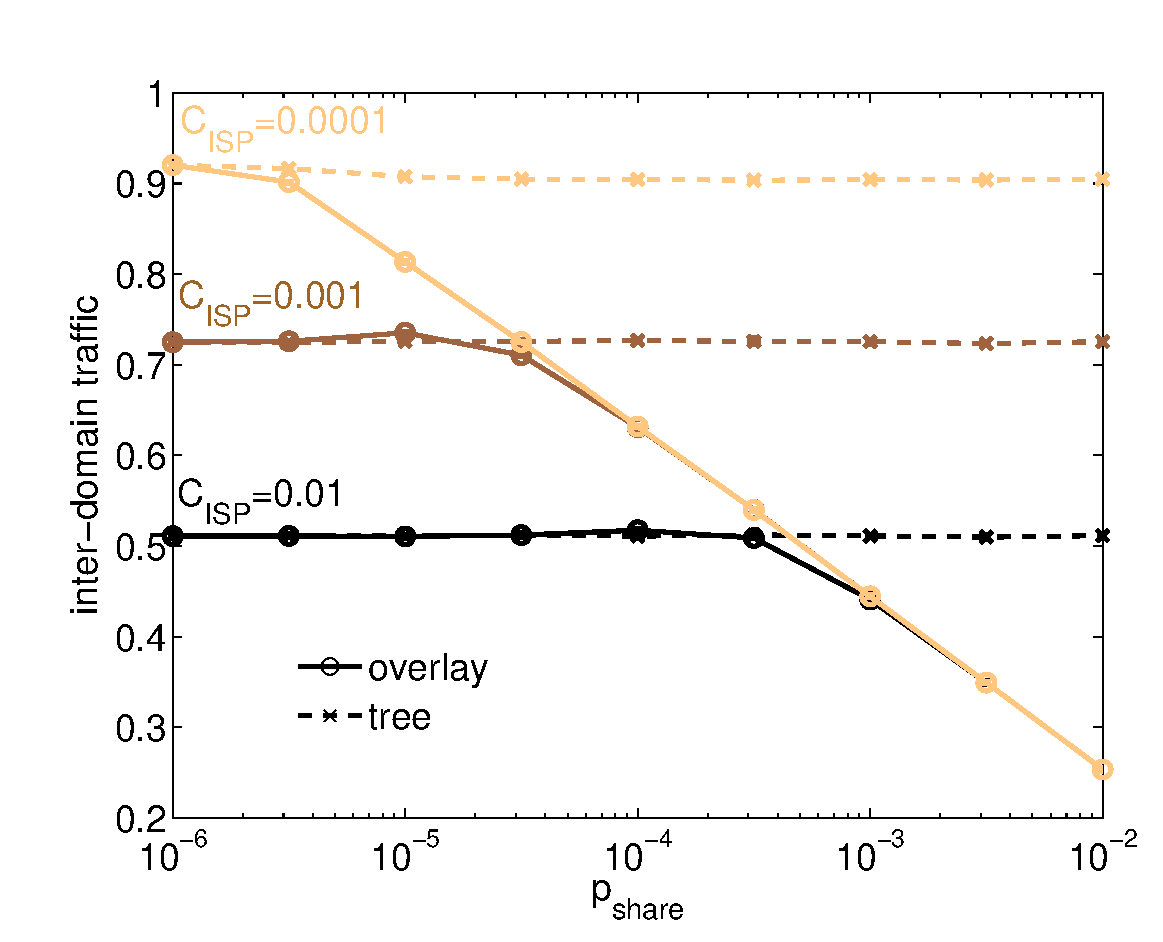
\includegraphics[width=0.7\textwidth]{hierarchical/simulative/figures/overlay_interdomain3}
  \caption{Inter-domain traffic dependent on home router sharing probability.}
  \label{fig:overlay_interdomain}
\end{figure}

% \begin{figure*}[tb]
% \centering
% \begin{subfigure}[t]{0.49\textwidth}
% 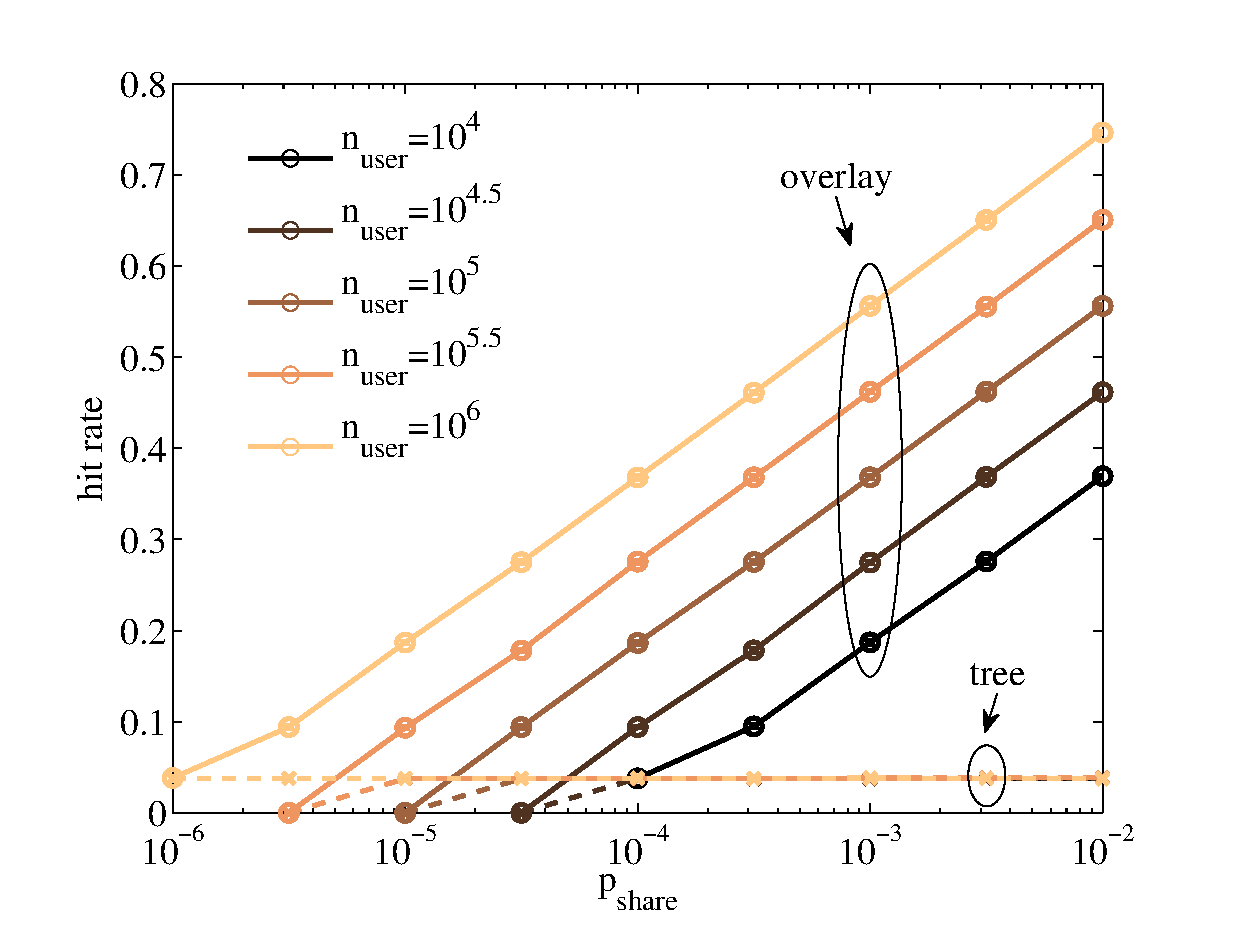
\includegraphics[width=\textwidth]{hierarchical/simulative/figures/overlay_nuser_hitrate}
% \caption{Hit rate of the overlay}
% \label{fig:overlay_nuser_hitrate}
% \end{subfigure}
% \begin{subfigure}[t]{0.49\textwidth}
% 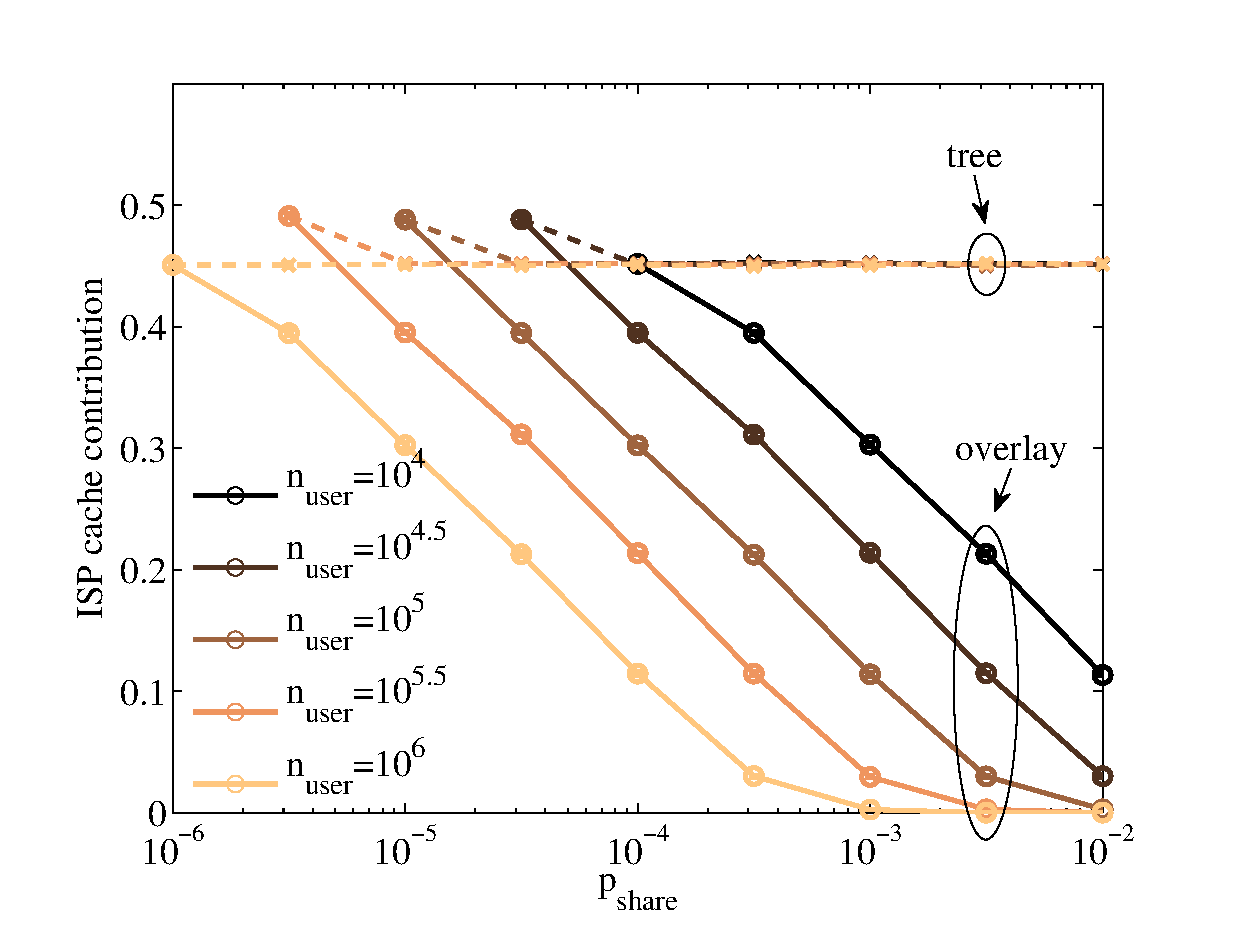
\includegraphics[width=\textwidth]{hierarchical/simulative/figures/overlay_nuser_ISPcontrib}
% \caption{ISP cache contribution}
% \label{fig:overlay_nuser_ISPcontrib}
% \end{subfigure}
% \begin{subfigure}[t]{0.49\textwidth}
% 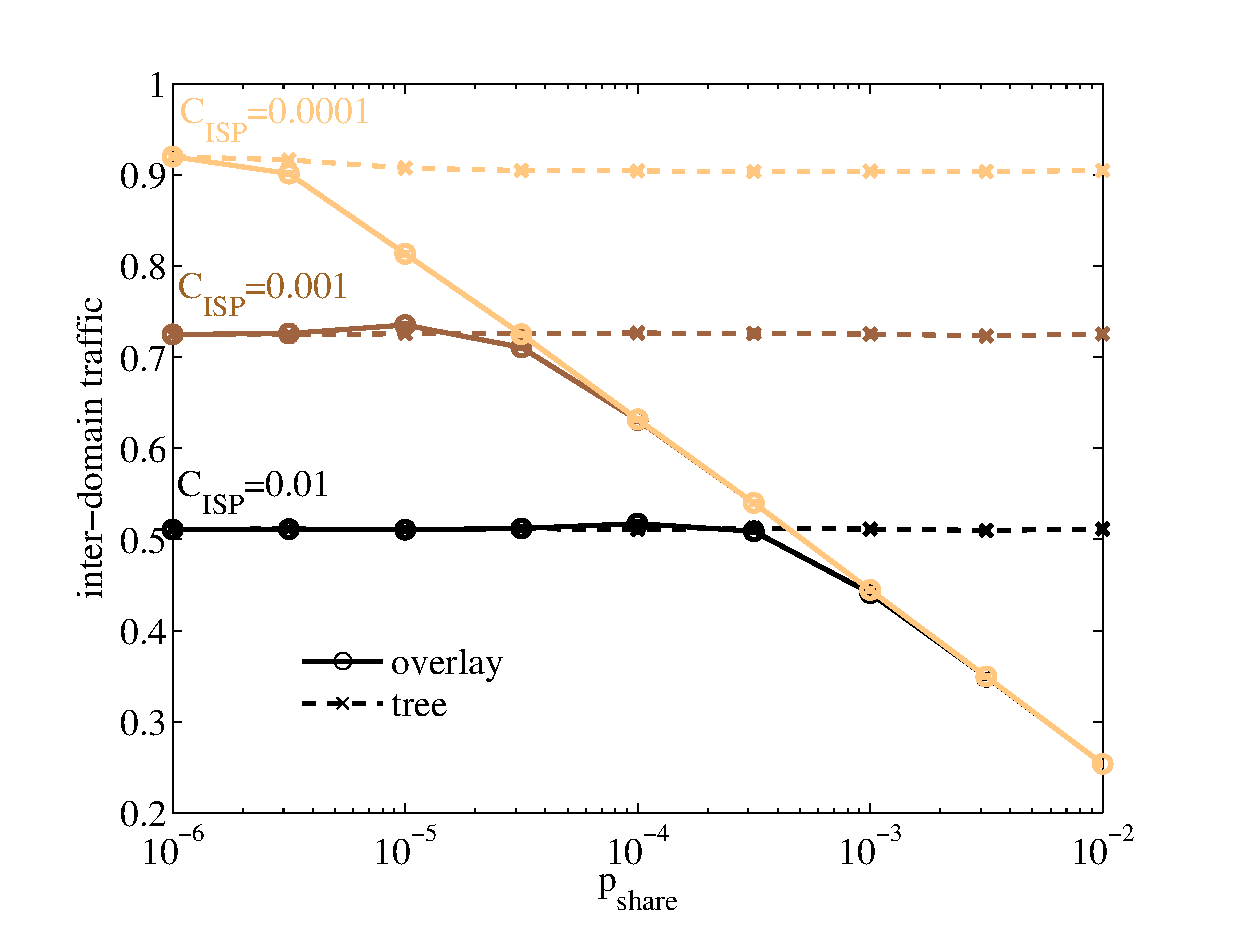
\includegraphics[width=\textwidth]{hierarchical/simulative/figures/overlay_interdomain}
% \caption{Inter-domain traffic}
% \label{fig:overlay_interdomain}
% \end{subfigure}
% \caption{Overlay and ISP cache contribution and inter-domain traffic dependent on home router sharing probability.}
% \end{figure*}

As the goal of this evaluation is to assess the potential of the overlay and to identify success scenarios, the simulation model assumes that the upload rate of caches is unlimited. However, in practice the upload rate limits the number of requests that can be served by a cache, especially for smaller devices like HRs. The evaluation uses a static and global popularity distribution. In practice the item request process is dynamic and dependent on personal and regional preferences.
The simulation uses a catalog size of $N=10^6$. The results obtained show the average of ten simulation runs with $10^6$ requests and their respective 95\% confidence intervals.
%The hierarchic caching strategy is leave-copy-down, which means that the video is cached in a certain tier only if it is already available in a higher tier.
%In the following we evaluate the performance of the tiered caching architecture. By studying the impact of the home router sharing probability, we identify the amount of home routers, which needs to be shared so that such a mechanism pays off for ISPs. We vary the ISP cache capacity and the Zipf exponent \alpha to investigate to what extent the load on ISP caches can be reduced and how the system performs under various request patterns. For each configuration 5 simulation runs were conducted to achieve significance. The results show the mean value of the 5 runs with 95\% confidence intervals.

Figure~\ref{fig:overlay_nuser_hitrate} shows the hit rate of the overlay dependent on the sharing probability for a constant ISP cache capacity of $C_\text{ISP}=0.01$. In the tree case, where each user is assigned to a HR as a tier-3 cache, the hit rate is independent of the sharing probability. The hit rate is limited by the cache capacity of the HR. If HRs are organized in an overlay, their hit rate increases with the sharing probability, since requested content items are looked up in all HRs belonging to the overlay. This shows that an overlay highly increases the performance of a caching system with a high number of small caches. Hence, the overlay highly benefits providers and end-users. The hit rate increases with the size of AS $n_\text{user}$, as a higher total cache capacity is available.

%\begin{figure}[tb]
%\centering
%\includegraphics[width=75mm]{overlay_ISPhitrate}
%\caption{ISP cache hit rate dependent on sharing probability.}
%\label{fig:overlay_ISPhitrate}
%\end{figure}

%Figure~\ref{fig:overlay_ISPhitrate} shows the ISP cache hit rate dependent on the home router sharing probability. The ISP cache hit rate decreases in the overlay case, since popular items are served by the overlay. The ISP cache is only requested for unpopular items which are less likely to be hit. Without overlay the ISP cache gets more efficient with increasing sharing probability, since the branching factor of the tree increases.

%\begin{figure}[tb]
%\centering
%\includegraphics[width=75mm]{overlay_ISPcontrib}
%\caption{ISP cache contribution dependent on sharing probability.}
%\label{fig:overlay_ISPcontrib}
%\end{figure}

Figure~\ref{fig:overlay_nuser_ISPcontrib} shows the ISP cache contribution dependent on the sharing probability for a constant ISP cache capacity of $C_\text{ISP}=0.01$. In a tree structure the sharing probability has no significant impact on the ISP cache contribution. This depends on the fact that the hit rate of tier-3 caches is low and independent of the sharing probability. All remaining requests are forwarded to the ISP cache and in case of a hit the ISP cache contributes. If the HRs are organized in an overlay, the ISP cache contribution decreases because more requests can be served from the overlay. In this case the ISP cache also gets less efficient because it is only requested for rare items that are not cached in the overlay.
For large ASs with a high number of end-users the ISP cache contribution approaches zero, if at least every thousandth user shares its HR. In this case the ISP cache can be shut down, which saves operating costs and energy. This shows that especially large ASs can benefit from an overlay.

%\begin{figure}[tb]
%\centering
%\includegraphics[width=75mm]{overlay_local}
%\caption{Share of requests served locally dependent on sharing probability.}
%\label{fig:overlay_ISPcontrib}
%\end{figure}

Figure~\ref{fig:overlay_interdomain} shows the inter-domain traffic dependent on the sharing probability for an AS with $n_\text{user}=10^6$ end-users. If no overlay is present the sharing probability has close to no impact on the amount of requests served locally. In this case the inter-domain traffic can only be reduced by increasing the ISP cache capacity. In the overlay case the number of requests served locally increases with the sharing probability, which decreases the inter-domain traffic. Dependent on the ISP cache capacity a higher fraction of shared HRs is necessary to reduce inter-domain traffic.

\subsubsection{Inter-Domain Traffic}

The overlay is not only used to access content from HRs in the same AS, but also from HRs in neighboring ASs. If the neighboring AS is a peering or customer ISP, no transit costs are incurred.
To assess the inter-domain traffic saved, an AS topology is added to the simulation. The AS relationship dataset provided by caida.org\cite{caida2015} of January 2015 is used and it specifies peering and customer-to-provider links of each AS. The data set consists of 46,172 ASs and 177,000 links.
To be able to process the simulation the topology is limited to RIPE NCC EU ASs. The remaining subset still consists of 31,256 ASs and 77,382 links.
The number of users per AS is determined by evaluating the Internet Census Dataset\cite{carna2013}, which provides a scan on active IP addresses in the Internet. Assuming that the number of users in an AS is proportional to the number of active IP addresses and the probability of a user being in an AS is set accordingly.
To save costly inter-domain traffic and to mitigate load on ISP caches, the following resource selection policy is applied:

If an item is not found on enabled HRs in the same AS, it is requested from other resources in the order:
%(1) HRs in peering ISP ASs, (2) HRs in customer ISP ASs, (3) ISP cache in local AS, (4) ISP cache in peering ISP ASs, (5) ISP cache in customer ISP ASs, and (6) content provider.
%\vspace{2mm}
\begin{enumerate}
	\itemsep0em
	\item HRs in peering ISP ASs
	\item HRs in customer ISP ASs
	\item ISP cache in local AS
	\item ISP cache in peering ISP ASs
	\item ISP cache in customer ISP ASs
	\item content provider
\end{enumerate}

\begin{figure}[tb]
  \centering
  \includegraphics[width=0.7\textwidth]{hierarchical/simulative/figures/RBHlocal3}
  \caption{Share of requests served locally dependent on sharing probability.}
  \label{fig:RBHlocal}
\end{figure}

\begin{figure}[tb]
  \centering
  \includegraphics[width=0.7\textwidth]{hierarchical/simulative/figures/ISPcontrib3}
  \caption{ISP cache contribution dependent on sharing probability.}
  \label{fig:ISPcontrib}
\end{figure}

\begin{figure}[tb]
  \centering
  \includegraphics[width=0.7\textwidth]{hierarchical/simulative/figures/RBHall3}
  \caption{Share of requests served per domain.}
  \label{fig:RBHall}
\end{figure}

% \begin{figure*}[ht]
% \centering
% \begin{subfigure}[t]{0.49\textwidth}
% \includegraphics[width=\textwidth]{hierarchical/simulative/figures/RBHlocal}
% \caption{Share of requests served locally}
% \label{fig:RBHlocal}
% \end{subfigure}
% \begin{subfigure}[t]{0.49\textwidth}
% \includegraphics[width=\textwidth]{hierarchical/simulative/figures/ISPcontrib}
% \caption{ISP cache contribution}
% \label{fig:ISPcontrib}
% \end{subfigure}
% \begin{subfigure}[t]{0.49\textwidth}
% \includegraphics[width=\textwidth]{hierarchical/simulative/figures/RBHall}
% \caption{Share of requests served per domain}
% \label{fig:RBHall}
% \end{subfigure}
% \caption{Share of requests served locally and ISP cache contribution dependent on sharing probability and share of requests served per domain.}
% \end{figure*}

A policy designed to prioritize ISP caches to remote HRs did not have a significant impact on traffic savings.
%The capacity of ISP caches $C_\text{ISP}=\{0.001,0.01\}$ is relative to the catalogue size.
The threshold $\theta$ specifies the minimum number of users an AS must have to host an ISP cache. If $\theta=\infty$ no AS hosts an ISP cache and content delivery is solely supported by HRs.
To investigate the performance of our approach, the impact of the HR sharing probability $p_\text{share}$ on the inter-domain traffic and on the ISP cache contribution is studied. The share of traffic within the local AS, peering and customer-to-provider links is evaluated.
For the generation of content item requests a Zipf popularity distribution with slope $\alpha=0.99$ was applied.

%\begin{figure}[tb]
%\centering
%\includegraphics[width=75mm]{RBHlocal}
%\caption{Share of requests served locally dependent on sharing probability.}
%\label{fig:RBHlocal}
%\end{figure}

Figure~\ref{fig:RBHlocal} shows the share of requests served locally dependent on the HR sharing probability. More than 20\% of requests can be served locally, if the ISP cache can store 1\% of the catalog size. With an increasing threshold $\theta$ the number of ASs hosting an ISP cache decreases and, thus, the share of requests being served locally. If the number of shared HRs increases, more traffic can be kept locally. This effect is stronger for a lower ISP cache capacity. In case of $\theta=\infty$ where no ISP caches are available, the sharing probability has the strongest impact on inter-domain traffic. For a high sharing probability the ISP cache size has only little impact on the inter-domain traffic.

Figure~\ref{fig:ISPcontrib} shows the ISP cache contribution dependent on the HR sharing probability. The number of requests an ISP cache can serve increases with its capacity. As for the inter-domain traffic, the sharing probability has a high impact on the ISP cache contribution. For high sharing probabilities the ISP cache contribution approaches zero. This means that ISP caches can be shut down, if a sufficient amount of users would share their HRs.
For a lower threshold $\theta$ more ISP caches are deployed and the ISP cache contribution increases.

%\begin{figure}[tb]
%\centering
%\includegraphics[width=75mm]{RBHall}
%\caption{Share of requests served per domain.}
%\label{fig:RBHall}
%\end{figure}

To study the requests served per domain, the HR sharing probability is set to 1\% and the threshold $\theta$ to 100 users.
Figure \ref{fig:RBHall} shows the share of requests served per domain. Almost none of these requests can be served by the personal HR. This might depend on the fact that items are requested according to a global popularity distribution.
If personal interests are considered in the demand model, higher hit rates and contributions from personal caches are expected. Dependent on the ISP cache capacity, 20 to 25\% of requests can be served locally and 15 to 20\% from neighboring ASs. Still about 2 out of 3 requests are served by the content provider. This depends on the fact that with Zipf slope of $\alpha = 0.99$ content item requests are highly heterogeneous. In practice, temporal and social dynamics of users' interests will lead to temporal and local correlations in requests, which improve the performance of local and personal caches.

%\input{aslevel/census/potential/potential}

\section{Lessons Learned}\label{sec:aslevel:lessons_learned}
In this chapter we characterize content delivery networks on autonomous systems level. %by evaluating measurements of the most common content delivery principles P2P and CDN.
For that purpose we summarize related work and use measurements conducted on the distributed platform PlanetLab and a crowdsourcing platform.
To assess the potential of content delivery approaches that use local resources, e.g., on home routers, we determine the number of active IP-addresses from the Internet Census dataset.

%P2P -> CDN
%to accurately model content delivery networks ... is described.
%While ... we find three major outcomes.
First, we provide a comprehensive overview on content delivery network concepts and their evolution. We briefly describe the structure of the YouTube CDN and describe the concept of the next generation of hierarchical CDNs, which use local resources to support content delivery.
In order assess the number of local resources available in each AS, we analyze the Internet Census Dataset to derive the distribution of IP-addresses on ASs.
To this end, we use a mapping of IP-addresses to autonomous system numbers.
we find that the distribution of IP-addresses is highly heterogeneous showing that 30\% of the active IPs belong to the 10 largest autonomous systems.
This means that the potential of approaches that use resources on home routers highly depend on the ISP network.

Second, we propose the usage of crowdsourcing platforms for distributed network measurements to increase the coverage of vantage points.
We evaluate the capability to discover global networks by comparing the coverage of video server detected, using a crowdsourcing platform as opposed to using the PlanetLab platform.
To this end, we use exemplary measurements of the global video CDN YouTube, conducted in both the PlanetLab platform as well as the crowdsourcing platform Microworkers.
Our results show that the vantage points of the concurring measurement platforms have very different characteristics.
We show that the distribution of vantage points has high impact on the capability of measuring a global content distribution network.
The capability of PlanetLab to measure a global CDNs is rather low, since 80\% of requests are directed to the United States.
Our results confirm that the coverage of vantage points is increased by crowdsourcing.
Using the crowdsourcing platform we obtain a diverse set of vantage points that reveals more than twice as many autonomous systems deploying video servers than the widely used PlanetLab platform.
%Part of future work is to determine if the coverage of vantage points can be even further increased by targeting workers from specific locations to get representative measurement points for all parts of the world.

Finally, we investigate where in the Internet BitTorrent traffic is located and which ISPs benefit from its optimization. To this end, we use measurements of live BitTorrent swarms to derive the location of BitTorrent peers and data provided by Caida.org in order to calculate the actual AS path between any two peers.
Our results show that the traffic optimization potential depends heavily on the type of ISP. Different ISPs will pursue different strategies to increase revenues.
Our results confirm that selecting peers based on their locality has a high potential to shorten AS paths between peers and to optimize the overlay network. In the observed BitTorrent swarms twice as much traffic can be kept intra-AS using locality peer selection. Thus, the inter-AS traffic is almost reduced by \unit[50]{\%} in \tier and in large ISPs.
%If ...
%This would for example allow ..

Based on the results obtained in this chapter, we develop models that describe the characteristics of CDNs and the number of active subscribers in ISP networks.
The models allow us to analyze the performance of traffic management mechanisms in realistic scenarios.
%Upper bounds / potential of p2p cdn approach.
%Including the application providers as stakeholders and considering their key performance indicators requires new models but also allows us to better understand the impact of mechanisms implemented in applications.
%Key performance indicators of application providers sometimes overlap with those relevant to users, as application providers try to improve the experience of users in order to reduce churn.

%Highlighted by both, the P2P approach and the CDN approach the distribution of peers on autonomous systems and the popularity of content is highly heterogeneous.
%Dynamics (orange paper)
%While general traffic management mechanisms intent to optimize the cdn
%this only increases the efficiency of the ISP cache, which may cause suboptimal results if the popularity of videos large variance.
%Thus, we suggest to  tradeoffs, within reason, to the user.
%This approach could be seen as extending the \emph{Economic Traffic Management} approach to the user.


\chapter{Analysis and Optimization of Hierarchical Caching Systems}\label{chap:hierarchical}

%The vast majority of Internet traffic is carried by content delivery networks (CDN).
%Major CDNs comprise of inter-connected data-centers at various points of presence around the world.
CDNs do not only carry a lot of traffic among the data-centers but also put huge loads on Internet Service Provider (ISP) networks that provide access to a high number of end-users consuming the content.
Reducing the traffic carried by CDNs and the load put on ISP networks has high potential to reduce energy consumption and cost for content delivery.
A common approach is to cache frequently requested content in or close to access networks to serve the content with low latency and few hops to save resources on the path.
%The current Internet architecture is designed to address servers which is a problem to enable efficient caching, since a server
%The field of content centric networking or information centric networking addresses this problem by making content addressable.
The content centric networking architecture proposes content caches on routers on the network path.
%when where which content requested
Caches have a limited capacity to store content, which means that content items stored on the cache need to be replaced if a newly requested item has to be stored in the cache.
%The key performance metric to optimize content delivery is the cache hit rate, which is the rate of requests that can be served by the cache directly in consequence of a cache hit, i.e., the content is stored on the cache at time of the request.

%Existing work \cite{} studies the cache replacement strategies that try to maximise the hit rate considering different performance indicators.
%Key indicator on the performance of caching strategies is the request process.
%Request processes in web services such as Video-on-Demand exhibit a power-law \cite{} as well as temporal \cite{} and spatial dynamics \cite{}.
A recent approach \cite{valancius2009greening} proposes to augment spare capacities on customer premise equipment (CPE) such as home routers or nano data-centers (NaDas) to assist content delivery, showing that there is a high potential to save energy, although the capacity of home gateways is small and the uplink is limited.
The content is transported in a peer-to-peer manner keeping the traffic within the AS.
Requests are first directed to the overlay of home gateways or NaDas, and is only forwarded to a cache of the content delivery network, if the target object is not found in the overlay.
In this way a hierarchy of caching systems is formed, in which the requests that cannot be served in one tier, i.e. the miss stream, is forwarded to the next tier in the hierarchy.
Another example for a hierarchical caching system with bandwidth constraints are femto caching architectures \cite{golrezaei2013femtocaching}, where content is cached on femto-basestations with small capacity but with considerable storage space.
The potential of these approaches highly depends on the number of caches available and their capacity for content delivery.
Our goal is to evaluate the performance of hierarchical content delivery networks using a high number of caches with limited capacity and to assess their potential to reduce inter-domain traffic.

sharing probability

%Leonardi infocom 2015 dynamic model

The performance of hierarchical cache networks can be accurately determined by analytic models developed in recent work \cite{che2002hierarchical, martina2014unified}.
The models do not consider constraints that limit the capability of caches to upload content such as the bandwidth of the uplink.
%In the NaDa approach the upload bandwidth of caches is limited.
To consider the upload bandwidth the system is modeled as loss network consisting of a server for each of the caches. The exact stationary distribution of the loss network is too complex to evaluate.
In \cite{tan2013optimal} the system is analyzed under large system asymptotic where simplifications occur.
We use a different approach by approximating the arrival rate of requests at the caches.
This allows us to effectively assess the loss probability by using a simple form of the Erlang formula for a loss network.
Even for traffic with highly heterogeneous request rates the approximation reflects the system performance.
To determine the number home gateways available to assist content delivery we rely on the insights gained from the characterization of Internet subscriptions on AS level in \refchap{chap:aslevel}.
 In order to assess the potential of hierarchical caching systems to reduce inter-domain traffic, we use the model for transit traffic described in \refchap{chap:aslevel}.

Our contribution is three-fold.
First, we provide a versatile simulation framework for evaluating hierarchical caching systems allowing to consider different features including the home router sharing probability, bandwidth constraints and the AS topology.
Second, we use the inferred AS paths to calculate the real AS paths and assess the transit cost savings by hierarchical caching systems.
Finally, we develop a method to accurately assess the system performance of tiered caching architectures with bandwidth constraints.

% \begin{figure}
%   \centering
%   \includegraphics{cloud/figures/hcmodel}
%   \caption{Stakeholders investigated in the cloud scenarios.}
%   \label{fig:hcmodel}
% \end{figure}


The content of this chapter is published in~\cite{info3-inproceedings-2015-518,info3-inproceedings-2015-530,info3-inproceedings-2015-514,burger2016hierarchical}.
\refsec{sec:hierarchical:related_work} gives an overview on related work on the performance evaluation of caching systems and describes traffic models and analytic methods, which are relevant for the evaluation of hierarchical caching systems.
We describe the simulation model in \refsec{sec:hierarchical:simulative:simulative} and discuss the results derived to assess the potential to save inter-domain traffic in \refsec{sec:hierarchical:simulative:evaluation}.
In \refsec{sec:hierarchical:analyticbw:model} we describe our method to evaluate the performance of hierarchical systems with bandwidth constraints and give analytic results.
Numerical examples derived by analysis and simulation are given in \refsec{sec:hierarchical:analyticbw:results}.
%The simulation framework for a tiered caching architecture is described in Section~\ref{sec:simulation}.
Finally, \refsec{sec:cloud:lessons_learned} summarizes this chapter and presents the lessons learned.

\section{Background and Related Work}\label{sec:p2p:background}

This section describes background of this chapter and presents related work. We start with an overview on measurement studies of live BitTorrent networks and show different approaches to reduce inter-ISP traffic discussed in the ALTO working group of the IETF. Finally, we introduce studies that infer the inter-AS relations based on BGP routing information.
We briefly describe the structure of the YouTube video CDN and give a short introduction in the principles of crowdsourcing.
Further, we summarize related work in the field of distributed active measurements of CDNs as well as work related to crowdsourcing aided network measurements.

\subsection{Measurements and Models of Live BitTorrent Networks}

BitTorrent is a peer-to-peer file-sharing protocol, which is based on multi-source downloads between the users. All the users, i.e., \textit{peers}, sharing the same file belong to a \textit{swarm}. To join the swarm, a peer requests addresses of other peers at an index server called \textit{tracker}. In the standard BitTorrent algorithm the tracker uses random peer selection to select a subset of peers that are in the swarm. Then, the joining peer tries to establish a neighbor relation to the peers it got from the tracker and collects all peers which accepted the request in his \textit{neighbor} set. The peer signals interest to all neighbors which have parts of the file it still needs to download. To which neighbor a peer is willing to upload data is decided by the choking algorithm, which is explained in \cite{cohen:bt}.

As basis of our methodology for modeling inter-ISP BitTorrent traffic, the results in \cite{Hossfeld2011} are revisited. In \cite{Hossfeld2011} the authors provide measurements of a large number of live BitTorrent swarms taken from popular index servers such as \emph{The Pirate Bay}, \emph{Mininova}, and \emph{Demonoid}. Using the IP addresses of the peers, the authors associate every peer with its AS and estimate the potential of ALTO mechanisms based on the differentiation between local peers (peers in the same AS) and remote peers located in other ASes. In contrast, we consider the actual Internet topology in this work, i.e., the inter-ISP relations, the ISP classification in the Internet hierarchy, and the AS paths between the peers in order to estimate the optimization potential of ALTO mechanisms.

The authors of \cite{Kryczka2011} use the peer exchange protocol (PEX) in order to measure the neighbor set of all peers participating in a number of live BitTorrent swarms. Based on this information, they model the graph topology of the swarms and compare the structure to random graphs. They also investigate clustering of peers within ASes and countries, but do not focus on inter-AS relations and AS paths between peers as we do in this work.

In addition, there are measurement studies that examine and model distinct features of BitTorrent networks. In \cite{Izal2004}, a single swarm was measured for five months with a focus on the download times of the peers. Additional parameters such as the peer inter-arrival times in the swarm, their upload capacity and their online time are considered in \cite{Pouwelse2005}. The authors of \cite{Guo2005} investigate these parameters also in multi-swarm scenarios. Finally, \cite{Zhang2010} measures \unit[4.6]{million} torrents to provide an overview of the entire BitTorrent ecosystem with its different communities and index servers. Our study differs from these works in that it focuses on the location of the peers in the Internet and the AS paths between the peers.

\subsection{ALTO Mechanisms and Their Performance Evaluation}

Various mechanisms to reduce the inter-ISP traffic generated by BitTorrent and other P2P applications are currently being investigated. Besides caching of BitTorrent traffic \cite{Lehrieder2010a,Lehrieder2012,Pacifici2012}, which might involve legal issues, changing standard BitTorrent algorithms is a promising approach. The authors of \cite{Aggarwal2007} propose to use an oracle service provided by the ISP guiding the peers in their peer selection process. The evaluation uses a Gnutella network and shows that intra-AS traffic is increased significantly without a negative impact on the overlay graph. Similar approaches are proposed for BitTorrent. Bindal et al. \cite{Bindal2006} reduce the inter-ISP traffic by modifying the neighbor set of the BitTorrent peers, which can be done at the tracker or enforced by the ISPs using deep packet inspection. Their simulations use a uniform peer distribution over ASes and show a high optimization potential of this approach. The authors of \cite{Xie2008} propose to use \emph{iTrackers} to guide the peers and formulates an optimization problem to find the best neighbor sets. Finally, Oechsner et al. \cite{Oechsner2009} propose to change the choke algorithm of BitTorrent to further reduce inter-ISP traffic and evaluate it via simulations in homogeneous scenarios. The BitTorrent plugin \emph{Ono} \cite{Choffnes2008} uses the servers of content distribution networks (CDN) as landmarks and estimates the proximity of two peers by the similarity of the CDN re-direction behavior.

The authors of \cite{gkantsidis2006planet} investigate analytically the capabilities of a P2P-based content distribution network and the impact of locality. In contrast to our work, they use traffic characteristics which arise from software updates and do not consider AS relationships.
A set of evaluations of ALTO mechanisms uses scenarios inspired by measurements of live BitTorrent swarms \cite{Cuevas2011,Blond2011,Lehrieder2011}. The studied scenarios consider heterogeneous peer distributions where some ASes contain more peers of a specific swarm than others. Nevertheless, they do not take into account inter-AS relations and the AS paths between two peers. This is different in our study. Using the AS affiliation of peers and the data obtained from Caida.org, we infer the actual paths of the BitTorrent connections in the Internet. In addition, we focus on the inter-ISP relations and investigate to which degree selfish ISPs profit from recommending their peers to preferentially use connections to peers located in lower tier ASes.

\subsection{Measurements of AS Relations and Topologies}

Autonomous systems are individual parts of the Internet, which are operated by ISPs.
On a technical level, the traffic exchange between the ASes is controlled by the Border Gateway Protocol (BGP)\cite{trangia2009}. However, commercial relations between ISPs determine the routing policies configured via BGP.
%The traffic exchanged between autonomous systems is inter-domain traffic. It is differentiated from intra-domain traffic, which is the traffic in the autonomous system.
An ISP must buy transit services to access parts of the Internet it neither owns nor can access by its customers.
Hence, to route traffic between autonomous systems ISPs engage in business relationships.
These business relationships are usually not open for public but they can be abstracted into three common types \cite{gao2001}.
The relationship between two ASes can be customer-to-provider (c2p), peer-to-peer (p2p) or sibling-to-sibling (s2s).
A customer-to-provider link is present if the customer AS pays the provider AS for transit service, i.e., the provider forwards the traffic of the customer and its customers. In a peer-to-peer relation the ASes have an agreement that they exchange each others traffic and the traffic of their customers, without paying each other. Sibling-to-sibling are links between ASes of the same organization. These relations are defined in business agreements and kept secret, but they can be inferred by analyzing the routing between autonomous systems.

The approach that is most widely used to infer AS relationships is analyzing BGP routing tables. The data set used in this work is also produced by inferring BGP tables as described in \cite{dimitropoulos2007relationships}. Therefore, AS links are extracted from RouteViews BGP tables. First sibling-to-sibling links are identified by looking up organizations that own multiple AS numbers. Then customer-to-provider relationships are inferred by a heuristic that is based on the idea of relaxing the requirement for a maximal number of valid paths and using the AS degree information to detect paths that are invalid. Most challenging is the inference of peer-to-peer links since paths remain valid if peer-to-peer links are replaced by a customer-to-provider or provider-to-customer link. The authors of \cite{dimitropoulos2007relationships} develop a heuristic which combines the strengths of previous approaches by \cite{gao2001} and \cite{di2003computing}. The inferred relationships were validated by surveys, showing that \unit[96.5]{\%} customer-to-provider, \unit[82.8]{\%} peer-to-peer, and \unit[90.3]{\%} sibling-to-sibling of the inferred relationships are correct.

\subsection{Evolution and Structure of Content Delivery Networks}
%To understand why distributed measurements are necessary and to provide the basic ideas of content delivery network structures, we briefly describe the evolution of content delivery networks and the functionality of the YouTube CDN.
Since the launch of the YouTube service content delivery has drastically changed.
While the amount of traffic transported over peer-to-peer networks remained about the same, the traffic transported by content delivery networks has increased exponentially \cite{cisco2015}.
The number of users watching videos on demand has massively increased and the bandwidth to access videos is much higher.
Furthermore, the increased bandwidth enables web services to be interactive by using dynamic server- or client-side scripts.
The appearance of dynamic services and the increasing quality of multimedia content raised user expectations and the demand on the servers.
To bring content in high quality to end-users with low latency and to deal with increasing demand, content providers have to replicate and distribute the content to get it close to end-users.
Thus, content delivery networks such as the Google CDN evolved.

The global expansion of the CDNs also changes the structure of the Internet.
Google has set up a global backbone which interconnects Google's data centers to important edge points of presence.
Since these points of presence are distributed across the globe, Google can offer direct peering links to access networks with many end users.
Such, access network providers save transit costs, while Google is able to offer services with low latency.
To bring content even closer to users ISPs can deploy Google servers inside their own network to serve popular content, including YouTube videos~\cite{gcc}.

To select the closest server for a content request and to implement load balancing CDNs use the Domain Name System (DNS).
Typically a user watches a YouTube video by visiting a YouTube video URL with a web browser.
The browser then contacts the local DNS server to resolve the hostname.
Thereafter, the HTTP request is directed to a front end web server that returns an HTML page including URLs for default and fallback video servers.
These URLs are again resolved by DNS servers to physical video servers, which stream the content.
The last DNS resolution can happen repeatedly until a server with enough capacity is found to serve the request.
Thus, load balancing between the servers is achieved~\cite{adhikari2012vivisecting}.

\subsection{Crowdsourcing}
Crowdsourcing is an emerging service in the Internet that enables outsourcing jobs to a large, anonymous crowd of users~\cite{articles2013-113}.
So called \emph{Crowdsourcing platforms} act as mediator between the users submitting the tasks, the \emph{employers}, and the users willing to complete these tasks, the \emph{workers}.
All interactions between workers and employers are usually managed through these platforms and no direct communication exits, resulting in a very loose worker-employer relationship.
The complexity of Crowdsourcing tasks varies between simple transcriptions of single words~\cite{vonAhn2008} and even research and development tasks~\cite{innocentive}.
Usually, the task description are much more fine granular than in comparable forms in traditional work organization~\cite{conf2011-417}.
This small task granularity hold in particular for \emph{micro-tasks}, which can be completed within a few seconds to a few minutes.
These tasks are usually highly repetitive, e.g., adding textual descriptions to pictures, and are grouped in larger units, so called \emph{campaigns}.

\subsection{Distributed Measurements of }
There already exist a number of publications which study the structure of the YouTube CDN and its selection of video servers.
A distributed active measurement platform is necessary for these evaluation, because the CDN mechanisms consider the client locations, both geographical as well as in terms of the connected access network.
In \cite{torres2011dissecting} two university campus networks and three ISP networks were used to investigate the YouTube CDN from vantage points in three different countries.
The results show that locality in terms of latency is not the only factor for video server selection.

While the view of five different ISPs on a global CDN is still narrow, the authors of \cite{adhikari2011you} used PlanetLab  to investigate the YouTube server selection strategies and load-balancing.
They find that YouTube massively deploys caches in many different locations worldwide, placing them at the edge of the Google autonomous system or even at ISP networks.
The work is enhanced in \cite{adhikari2012vivisecting}, where they uncover a detailed architecture of the YouTube CDN, showing a 3-tier physical video server hierarchy.
Furthermore, they identify a layered logical structure in the video server namespace, allowing YouTube to leverage the existing DNS system and the HTTP protocol.

However, to assess the expansion of the whole YouTube CDN and its cache locations in access networks, the PlanetLab platform, which is located solely in NRENs, is not suitable, since it does not reflect the perspective of end users in ISP access networks.
Therefore, a different distributed measurement platform is used in \cite{rafetseder2011exploring} which runs on end user equipment and thus implies a higher diversity of nodes and reflects the perspective of end user in access networks.
However, the number of nodes that was available for the measurement is too small to obtain a global coverage of vantage points

To achieve both, the view of access networks and a high global coverage with a large number of measurement points, the participation of a large number of end users in the measurement is necessary.
Bischof et al. \cite{bischof2011crowdsourcing} implemented an approach to gather data form peer-to-peer networks to globally characterize the service quality of ISPs using volunteers.

In contrast to this we propose using a commercial crowdsourcing platform to recruit users running a specially designed measurement software and therewith act as measurement probes.
In comparison to other approaches using volunteers, this approach offers better scalability and controllability, because the number and origin of the participants can be adjusted using the recruiting mechanism of the crowdsourcing platform.
This is confirmed by Table~\ref{tab:CvsS} which compares a crowdsourcing study with a social network study quantitatively. The crowdsourcing study  is described in \cite{bookchapter2013-18}. The study is designed to assess the subjective QoE for multimedia applications, like video streaming.
The same study was conducted additionally in a social network environment for recruiting test users.
Table~\ref{tab:CvsS} shows that acquiring people in crowdsourcing platforms takes very short time compared to asking volunteers in a social network, which allows adding participants easily.
Furthermore, the completion time of the campaign of 31 hours is much shorter compared to the 26 days for the social network campaign.
Finally, in the crowdsourcing campaign workers can be selected according to their country, which allows distributing the campaign on many different countries. In the social network the coverage of countries depends on the network of user groups, which spread the campaign.
Hence, it is easy to control the number and origin of subjects participating in a crowdsourcing campaign and the completion time is considerably fast, which makes the campaign scalable and controllable. The price you pay is the reward for the workers that summed up to a total of 16 Euro for that campaign.

\begin{table}[tb]
\caption{Quantitative Comparison: Crowdsourcing / Social Network Study.} \label{tab:CvsS}
\begin{center}
{\footnotesize
	\begin{tabular}{|p{.29\textwidth}|p{.29\textwidth}|p{.29\textwidth}|} \hline
		\textbf{} & \textbf{Crowdsourcing (C)} & \textbf{Social network (S)} \\ \hline
		\textbf{Implementation time} & about 2 weeks; test implemented via dynamic web pages, application monitoring & same as for (C) \\ \hline
		\textbf{Time for acquiring people} & 5 minutes & 2 hours, as users (groups) were asked individually \\ \hline
		\textbf{Campaign submission cost} & 16 Euro & 0 Euro \\ \hline
		\textbf{Subject’s reward} & 0.15 Euro & 0 Euro \\ \hline
		\textbf{Number of test conditions} & 3 & 3 \\ \hline
		\textbf{Advertised  people} & 100 & 350 \\ \hline
		\textbf{Campaign completion time} & 31 hours & 26 days; strongly depends on advertised user groups however \\ \hline
		\textbf{Participating users} & 100 & 95 \\ \hline
		\textbf{Reliable users (very strict filtering of users)} & 30 & 58 \\ \hline
		\textbf{Number of different countries of subjects} & 30 & 3; strongly depends on users groups however \\ \hline
		\end{tabular}
}
\end{center}
\end{table}



The Internet Census Dataset was validated forensically in \cite{dainotticaida}.
In \cite{krenc2014internet} the scope of the dataset is taken into perspective and show that, although there are some qualitative problems, the measurement data seems to be authentic.
We use the Internet Census Dataset to determine the number of active IP-addresses for each autonomous system in the Internet.
%To the best of our knowledge, this is the first work which evaluates a gl
%To the best of our knowledge this is the first work which uses crowdsourcing for a distributed active measurement platform.

\section{Simulative Evaluation of Hierarchical Caching Systems}\label{sec:hierarchical:simulative:simulative}

We develop an event-based simulation framework to evaluate the performance of content delivery networks.
The results derived from the simulative evaluation are used to validate the analytic models.
The simulation framework further allows considering complex system characteristics in the performance evaluation that are not covered by the analytic models, such as the transit costs charged on inter-domain links.

%A hierarchical content delivery network with bandwidth constraints has been evaluated by simulation in \cite{applegate2010optimal}.
%The impact of using edge resources with limited capacity for content delivery on QoE is evaluated by means of simulation in \cite{info3-inproceedings-2015-530}.
In the following we describe the simulation model and investigate the benefit of overlays networks in hierarchical caching systems.
We use the model for transit traffic, c.f. \refsec{sec:p2p:methodology}, to assess the potential to save costs produced by inter-domain traffic.

\subsection{Simulation Model}\label{sec:simeval}

The parameters considered in the content delivery simulation framework are
\begin{enumerate}
  \itemsep0em
  \item the resource distribution,
  \item the caching and content placement strategy,
  \item the resource selection strategy,
  \item the content demand,
  \item the AS-Topology.
\end{enumerate}
Other considered parameters that are not relevant for this monograph, are
\begin{enumerate}
  \itemsep0em
  \item the social network of users,
  \item the video bitrate and chunk-size distribution,
  \item and the application and QoE.
\end{enumerate}
In the following we briefly describe each of the parameter sets and provide models.

\subsubsection{Resource Distribution}
The resource distribution determines how video streaming sources are distributed among autonomous systems.
The number and size of autonomous systems is specified.
The size of an autonomous system is given by the number of end-users located in it.
In literature, the distribution of end-users on ASs is characterized as heterogeneous \cite{Hossfeld2011}.
We use a geometric distribution as a basic model for number of end-users in the ASs.
A more detailed model is developed using the Internet Census dataset, c.f. \refsec{sec:aslevel:census}.
Video streaming sources can be a) data centers of the content provider, b) edge caches of the content provider, c) caches hosted by the ISP, d) home router / NaDas, or e) end-user devices.
For each video streaming source the AS-location and its capacity is specified.
The capacity is given by the number of items that can be cached.
The size of the item catalogue is also specified in this parameter set.

The cache resources can have bandwidth constraints specified by the mean and the standard deviation of the upload bandwidth.
If the upload bandwidth of a cache is limited, the service time of an object is calculated according to the available bandwidth and the object size.
The service times of the objects served by a cache are updated if the upload bandwidth changes or if an object request arrives or is completed.
Requests are blocked by a cache if the available bandwidth is below a certain threshold, or if the cache is busy serving a request.

\subsubsection{Caching and Content Placement Strategy}
The caching and content placement strategy determines in which video streaming source which video item is placed and when.
The content placement strategy is defined by the caching strategies of the individual caches.
In a distributed approach each cache decides based on the information it has, which items to cache.
Thus, the availability of items in ASs might for example be increased.
If global knowledge of the item demand is assumed, optimized content placement strategies such as hot warm cold can be used.
Each caching strategy is further defined by its specific parameters according to \refsec{sec:hierarchical:background:strategies}.

\subsubsection{Resource Selection Strategy}
The resource selection strategy determines from which cache instance an item is streamed when requested.
The simplest resource selection just selects a random resource.
In hierarchical content delivery networks, resources in tier-1 are selected first, by default.
Other resource selection strategies that try to optimize different metrics were implemented.
E.g., local resource selection tries to save inter-domain traffic by prioritizing caches in the order: home router / NaDa in the same AS, ISP managed cache in the same AS, edge cache of content provider, data center of content provider.
%Further resource selection strategies that are not yet implemented could for example consider load balancing of the request based on the capacity of the caches.

\subsubsection{Social Network of Users}
The social network of users determines the friendship relationships between users. A basic model only defines the number of users in the system.
The number of friends of the user can be modeled by a power-law or geometric distribution.
A more detailed model specifies the friendship graph which consists of a node for each user and edges between users with friend relationships.
Friendship graphs have typical properties, such as a heavy-tailed in and out degree distribution.
In literature are different models for generating graphs with these properties.
A model used to generate social network graphs with varying size and density is the forest fire model \cite{leskovec2005graphs}.
We further specify the feed size as parameter that represents the news feed of social network platforms.
The news feed is updated in sharing events.
Videos which are on the news feed of a user are watched with higher probability.
Categories are defined by specifying the probability that a user is interested in a particular category.

\subsubsection{Traffic and Popularity Model}
The content demand determines the request rates of the video items.
Different demand models are implemented in the simulation, that reach from basic models that only consider the popularity distribution of the items, to detailed models that consider temporal, spatial and social dynamics, c.f. \refsec{sec:hierarchical:background:traffic}.

The arrival process of video requests is specified by the inter-arrival time of video requests.
The request rate depends on the time of day and is generally lower at night.
The day is divided in short time slots, where the arrival rate does not change significantly, so that the arrival process can be assumed as quasi stationary.
In these time slots the arrival process is modeled as Poisson-process.
The parameter lambda of the arrival process depends on the popularity of the item and the time of day.
The probability of sharing a watched video is given by the sharing probability.

\subsubsection{Autonomous System Topology}
In order to estimate the amount of inter-domain traffic and transit costs produced, and AS topology with AS paths can be specified.
The AS paths connect the caches and data centers providing the content with the users consuming the content.
For that purpose the AS paths are inferred from AS relationships as in \refsec{sec:p2p:methodology}.
Assuming that the number of users is proportional to the number of IP addresses in an AS, we use the results of the Internet Census Dataset evaluation in \refsec{sec:aslevel:census}, to determine the distribution of users on ASs.

Finally, Simulation parameters are specified that define the random number seed, the simulation time and the parameter study.

\subsubsection{Performance metrics}

Of the total number of $n$ object requests to a cache, the objects of $k$ requests are stored in the cache and can potentially be served by the cache.
Due to bandwidth constraints some of the $k$ requests may be blocked, such that only $k'\leq k$ of the $n$ object requests are served by the cache.
To assess the performance of content delivery networks several metrics are considered:

\begin{enumerate}
\item Cache hit rate $p_\text{hit}$: The ratio of requests to a cache that find the object in the cache (cache hit) to the total number of requests to the cache
\begin{equation}
  p_\text{hit}=\frac{k}{n} \, .
\end{equation}
\item Cache serve rate $p_\text{serve}$: The ratio of requests to a cache that find the object in the cache and that are not blocked due to bandwidth constraints to the total number of requests to the cache
\begin{equation}
  p_\text{serve}=\frac{k'}{n} \, .
\end{equation}
\item Cache contribution: The share of all requests that is served by a cache.
\item Inter-domain traffic: The share of requests by users in an AS that cannot be served by a cache in the same AS.
\end{enumerate}

\begin{figure}[bt]
  \centering
  \includegraphics[width=0.8\textwidth]{hierarchical/simulative/figures/watch}
  \caption{Proccess diagram of a WATCH event.}
  \label{fig:WATCH}
\end{figure}

The content delivery simulation framework is implemented in MatLab.
The simulation is event-based including two major events.
First, the WATCH event, which is processed when a user watches or consumes a video item.
Second, the SHARE event, which simulates a sharing action of a user, where the video is posted on the news feeds in the social network.
\reffig{fig:WATCH} shows the process diagram of a WATCH event.
The process of a WATCH event starts by selecting a video according to the specified demand model.
A video identifier $v_\text{id}$ is returned.
In the next step a cache or data center is selected according to the resource selection strategy that holds the item with $v_\text{id}$.
The download of the item from the selected resource is recorded in the statistics.
The cache identifier $c_\text{id}$ is returned and the cached items are updated according to the caching strategy specified in the parameters.
The user then decides to share $v_\text{id}$ with probability $p_\text{share}$.
In this case a SHARE event is queued.
Finally, the next WATCH event is queued according to the traffic and popularity model.

A SHARE event puts a given $v_\text{id}$, or a random video according to the user's interest on top of the news feed of the user's friends.
The user's friends are determined by the social graph.
The simulation is initialized with a WATCH event for each user.

The simulation framework is open source and available on github\footnote{\url{https://github.com/pettitor/content_delivery}}.

\subsection{Numerical Examples and Impact on Transit Costs}\label{sec:hierarchical:simulative:evaluation}

To evaluate the performance of a CDN supported by home routers, two scenarios are simulated. The first scenario simulates requests to a CDN with caches organized in a tree structure and compares isolated caches to cooperating caches to assess the benefit of the overlay.
The second scenario adds an AS topology with peering and transit links to evaluate the inter-domain traffic saving potential.
As described in \refchap{chap:aslevel}, a transit link exists between a customer ISP and its transit provider, if the customer ISP pays the transit provider to forward its traffic destined to parts of the Internet that the customer ISP does not own or cannot reach.

%\subsection{Caching}
% To assess the impact of the number of shared home routers and the size of the ISP, a tiered caching architecture with resource locations at three different tiers, including the main data center of the content provider, CDN caches, and end-user equipment is evaluated.
% The number of different content items to be downloaded or streamed from the resources is specified by the catalog size $N$. Tier-3 resource is the data center of the content provider, where all $N$ content items are stored. Tier-2 resources are edge caches and ISP caches, typically organized in a CDN, which are located close to Internet exchange points or within ISP networks. Requests served by ISPs or edge caches produce less or no inter-domain costs. Thus, these caches are referred as ISP caches in the following. The capacity of ISP caches is given as a fraction of $N$ and is specified by $C_\text{ISP}$. The caching strategy of ISP caches is LRU.
%Each autonomous system hosts an ISP cache.
Within tier-1, the caches are placed on shared home routers. These caches are referred to in the following as home routers (HRs). The cache capacity of HRs is specified by $C_1$ and their caching strategy is LRU. In this study $C_1$ is set to four (4) content items.
We evaluate the performance dependent on the autonomous system size $n_\text{user}$, in terms of the number of end-users in the autonomous system. The probability that an end-user enables the HR to shares contents is given by $p_\text{share}$. The probability that a user requests certain content items depends on the content's popularity distribution, which is specified by the Zipf exponent $\alpha$.

\subsubsection{Benefits of an Overlay}

To evaluate the performance of the overlay, two cases are considered (a) the tree case and (b) the overlay case. In the tree case (a), each user is assigned to one shared HR in its AS. If a user shares its HR, it is assigned only to its HR. A requested item is looked up in the assigned HR initially, i.e. in the tier-3 cache. If the requested item is not found, the request is forwarded to the next tier. The hierarchical caching strategy is leave-copy-everywhere, which means that the video is cached in each cache on the look up path. In the overlay case (b), a requested item is looked up in the HR of the user, if it is not found, it is looked up in shared HRs in the same autonomous system using the overlay. If no tier-3 cache in the AS contains the item it is looked up in tier-2 caches and finally in the data center of the content provider. The hierarchical caching strategy is leave-copy-everywhere, too, with the constraint, that the item is cached in the tier-3 cache only, which was looked up first.

\begin{figure}[tb]
  \centering
  \includegraphics[width=0.7\textwidth]{hierarchical/simulative/figures/overlay_nuser_hitrate3}
  \caption{Hit rate of the overlay dependent on home router sharing probability.}
  \label{fig:overlay_nuser_hitrate}
\end{figure}

\begin{figure}[tb]
  \centering
  \includegraphics[width=0.7\textwidth]{hierarchical/simulative/figures/overlay_nuser_ISPcontrib3}
  \caption{ISP cache contribution dependent on home router sharing probability.}
  \label{fig:overlay_nuser_ISPcontrib}
\end{figure}

\begin{figure}[tb]
  \centering
  \includegraphics[width=0.7\textwidth]{hierarchical/simulative/figures/overlay_interdomain3}
  \caption{Inter-domain traffic dependent on home router sharing probability.}
  \label{fig:overlay_interdomain}
\end{figure}

% \begin{figure*}[tb]
% \centering
% \begin{subfigure}[t]{0.49\textwidth}
% \includegraphics[width=\textwidth]{hierarchical/simulative/figures/overlay_nuser_hitrate}
% \caption{Hit rate of the overlay}
% \label{fig:overlay_nuser_hitrate}
% \end{subfigure}
% \begin{subfigure}[t]{0.49\textwidth}
% \includegraphics[width=\textwidth]{hierarchical/simulative/figures/overlay_nuser_ISPcontrib}
% \caption{ISP cache contribution}
% \label{fig:overlay_nuser_ISPcontrib}
% \end{subfigure}
% \begin{subfigure}[t]{0.49\textwidth}
% \includegraphics[width=\textwidth]{hierarchical/simulative/figures/overlay_interdomain}
% \caption{Inter-domain traffic}
% \label{fig:overlay_interdomain}
% \end{subfigure}
% \caption{Overlay and ISP cache contribution and inter-domain traffic dependent on home router sharing probability.}
% \end{figure*}

As the goal of this evaluation is to assess the potential of the overlay and to identify success scenarios, the simulation model assumes that the upload rate of caches is unlimited. However, in practice the upload rate limits the number of requests that can be served by a cache, especially for smaller devices like HRs. The evaluation uses a static and global popularity distribution. In practice the item request process is dynamic and dependent on personal and regional preferences.
The simulation uses a catalog size of $N=10^6$. The results obtained show the average of ten simulation runs with $10^6$ requests and their respective 95\% confidence intervals.
%The hierarchic caching strategy is leave-copy-down, which means that the video is cached in a certain tier only if it is already available in a higher tier.
%In the following we evaluate the performance of the tiered caching architecture. By studying the impact of the home router sharing probability, we identify the amount of home routers, which needs to be shared so that such a mechanism pays off for ISPs. We vary the ISP cache capacity and the Zipf exponent \alpha to investigate to what extent the load on ISP caches can be reduced and how the system performs under various request patterns. For each configuration 5 simulation runs were conducted to achieve significance. The results show the mean value of the 5 runs with 95\% confidence intervals.

Figure~\ref{fig:overlay_nuser_hitrate} shows the hit rate of the overlay dependent on the sharing probability for a constant ISP cache capacity of $C_\text{ISP}=0.01$. In the tree case, where each user is assigned to a HR as a tier-3 cache, the hit rate is independent of the sharing probability. The hit rate is limited by the cache capacity of the HR. If HRs are organized in an overlay, their hit rate increases with the sharing probability, since requested content items are looked up in all HRs belonging to the overlay. This shows that an overlay highly increases the performance of a caching system with a high number of small caches. Hence, the overlay highly benefits providers and end-users. The hit rate increases with the size of AS $n_\text{user}$, as a higher total cache capacity is available.

%\begin{figure}[tb]
%\centering
%\includegraphics[width=75mm]{overlay_ISPhitrate}
%\caption{ISP cache hit rate dependent on sharing probability.}
%\label{fig:overlay_ISPhitrate}
%\end{figure}

%Figure~\ref{fig:overlay_ISPhitrate} shows the ISP cache hit rate dependent on the home router sharing probability. The ISP cache hit rate decreases in the overlay case, since popular items are served by the overlay. The ISP cache is only requested for unpopular items which are less likely to be hit. Without overlay the ISP cache gets more efficient with increasing sharing probability, since the branching factor of the tree increases.

%\begin{figure}[tb]
%\centering
%\includegraphics[width=75mm]{overlay_ISPcontrib}
%\caption{ISP cache contribution dependent on sharing probability.}
%\label{fig:overlay_ISPcontrib}
%\end{figure}

Figure~\ref{fig:overlay_nuser_ISPcontrib} shows the ISP cache contribution dependent on the sharing probability for a constant ISP cache capacity of $C_\text{ISP}=0.01$. In a tree structure the sharing probability has no significant impact on the ISP cache contribution. This depends on the fact that the hit rate of tier-3 caches is low and independent of the sharing probability. All remaining requests are forwarded to the ISP cache and in case of a hit the ISP cache contributes. If the HRs are organized in an overlay, the ISP cache contribution decreases because more requests can be served from the overlay. In this case the ISP cache also gets less efficient because it is only requested for rare items that are not cached in the overlay.
For large ASs with a high number of end-users the ISP cache contribution approaches zero, if at least every thousandth user shares its HR. In this case the ISP cache can be shut down, which saves operating costs and energy. This shows that especially large ASs can benefit from an overlay.

%\begin{figure}[tb]
%\centering
%\includegraphics[width=75mm]{overlay_local}
%\caption{Share of requests served locally dependent on sharing probability.}
%\label{fig:overlay_ISPcontrib}
%\end{figure}

Figure~\ref{fig:overlay_interdomain} shows the inter-domain traffic dependent on the sharing probability for an AS with $n_\text{user}=10^6$ end-users. If no overlay is present the sharing probability has close to no impact on the amount of requests served locally. In this case the inter-domain traffic can only be reduced by increasing the ISP cache capacity. In the overlay case the number of requests served locally increases with the sharing probability, which decreases the inter-domain traffic. Dependent on the ISP cache capacity a higher fraction of shared HRs is necessary to reduce inter-domain traffic.

\subsubsection{Inter-Domain Traffic}

The overlay is not only used to access content from HRs in the same AS, but also from HRs in neighboring ASs. If the neighboring AS is a peering or customer ISP, no transit costs are incurred.
To assess the inter-domain traffic saved, an AS topology is added to the simulation. The AS relationship dataset provided by caida.org\cite{caida2015} of January 2015 is used and it specifies peering and customer-to-provider links of each AS. The data set consists of 46,172 ASs and 177,000 links.
To be able to process the simulation the topology is limited to RIPE NCC EU ASs. The remaining subset still consists of 31,256 ASs and 77,382 links.
The number of users per AS is determined by evaluating the Internet Census Dataset\cite{carna2013}, which provides a scan on active IP addresses in the Internet. Assuming that the number of users in an AS is proportional to the number of active IP addresses and the probability of a user being in an AS is set accordingly.
To save costly inter-domain traffic and to mitigate load on ISP caches, the following resource selection policy is applied:

If an item is not found on enabled HRs in the same AS, it is requested from other resources in the order:
%(1) HRs in peering ISP ASs, (2) HRs in customer ISP ASs, (3) ISP cache in local AS, (4) ISP cache in peering ISP ASs, (5) ISP cache in customer ISP ASs, and (6) content provider.
%\vspace{2mm}
\begin{enumerate}
	\itemsep0em
	\item HRs in peering ISP ASs
	\item HRs in customer ISP ASs
	\item ISP cache in local AS
	\item ISP cache in peering ISP ASs
	\item ISP cache in customer ISP ASs
	\item content provider
\end{enumerate}

\begin{figure}[tb]
  \centering
  \includegraphics[width=0.7\textwidth]{hierarchical/simulative/figures/RBHlocal3}
  \caption{Share of requests served locally dependent on sharing probability.}
  \label{fig:RBHlocal}
\end{figure}

\begin{figure}[tb]
  \centering
  \includegraphics[width=0.7\textwidth]{hierarchical/simulative/figures/ISPcontrib3}
  \caption{ISP cache contribution dependent on sharing probability.}
  \label{fig:ISPcontrib}
\end{figure}

\begin{figure}[tb]
  \centering
  \includegraphics[width=0.7\textwidth]{hierarchical/simulative/figures/RBHall3}
  \caption{Share of requests served per domain.}
  \label{fig:RBHall}
\end{figure}

% \begin{figure*}[ht]
% \centering
% \begin{subfigure}[t]{0.49\textwidth}
% \includegraphics[width=\textwidth]{hierarchical/simulative/figures/RBHlocal}
% \caption{Share of requests served locally}
% \label{fig:RBHlocal}
% \end{subfigure}
% \begin{subfigure}[t]{0.49\textwidth}
% \includegraphics[width=\textwidth]{hierarchical/simulative/figures/ISPcontrib}
% \caption{ISP cache contribution}
% \label{fig:ISPcontrib}
% \end{subfigure}
% \begin{subfigure}[t]{0.49\textwidth}
% \includegraphics[width=\textwidth]{hierarchical/simulative/figures/RBHall}
% \caption{Share of requests served per domain}
% \label{fig:RBHall}
% \end{subfigure}
% \caption{Share of requests served locally and ISP cache contribution dependent on sharing probability and share of requests served per domain.}
% \end{figure*}

A policy designed to prioritize ISP caches to remote HRs did not have a significant impact on traffic savings.
%The capacity of ISP caches $C_\text{ISP}=\{0.001,0.01\}$ is relative to the catalogue size.
The threshold $\theta$ specifies the minimum number of users an AS must have to host an ISP cache. If $\theta=\infty$ no AS hosts an ISP cache and content delivery is solely supported by HRs.
To investigate the performance of our approach, the impact of the HR sharing probability $p_\text{share}$ on the inter-domain traffic and on the ISP cache contribution is studied. The share of traffic within the local AS, peering and customer-to-provider links is evaluated.
For the generation of content item requests a Zipf popularity distribution with slope $\alpha=0.99$ was applied.

%\begin{figure}[tb]
%\centering
%\includegraphics[width=75mm]{RBHlocal}
%\caption{Share of requests served locally dependent on sharing probability.}
%\label{fig:RBHlocal}
%\end{figure}

Figure~\ref{fig:RBHlocal} shows the share of requests served locally dependent on the HR sharing probability. More than 20\% of requests can be served locally, if the ISP cache can store 1\% of the catalog size. With an increasing threshold $\theta$ the number of ASs hosting an ISP cache decreases and, thus, the share of requests being served locally. If the number of shared HRs increases, more traffic can be kept locally. This effect is stronger for a lower ISP cache capacity. In case of $\theta=\infty$ where no ISP caches are available, the sharing probability has the strongest impact on inter-domain traffic. For a high sharing probability the ISP cache size has only little impact on the inter-domain traffic.

Figure~\ref{fig:ISPcontrib} shows the ISP cache contribution dependent on the HR sharing probability. The number of requests an ISP cache can serve increases with its capacity. As for the inter-domain traffic, the sharing probability has a high impact on the ISP cache contribution. For high sharing probabilities the ISP cache contribution approaches zero. This means that ISP caches can be shut down, if a sufficient amount of users would share their HRs.
For a lower threshold $\theta$ more ISP caches are deployed and the ISP cache contribution increases.

%\begin{figure}[tb]
%\centering
%\includegraphics[width=75mm]{RBHall}
%\caption{Share of requests served per domain.}
%\label{fig:RBHall}
%\end{figure}

To study the requests served per domain, the HR sharing probability is set to 1\% and the threshold $\theta$ to 100 users.
Figure \ref{fig:RBHall} shows the share of requests served per domain. Almost none of these requests can be served by the personal HR. This might depend on the fact that items are requested according to a global popularity distribution.
If personal interests are considered in the demand model, higher hit rates and contributions from personal caches are expected. Dependent on the ISP cache capacity, 20 to 25\% of requests can be served locally and 15 to 20\% from neighboring ASs. Still about 2 out of 3 requests are served by the content provider. This depends on the fact that with Zipf slope of $\alpha = 0.99$ content item requests are highly heterogeneous. In practice, temporal and social dynamics of users' interests will lead to temporal and local correlations in requests, which improve the performance of local and personal caches.

%\input{hierarchical/analytic/analytic}
\section{Analysis of Caching Systems with Bandwidth Constraints}\label{sec:hierarchical:analyticbw:model}

To evaluate content delivery networks based on the number of available home routers and their limited capacity, we define a system model for a tiered caching architecture.
Tier-1 caches are on leaf nodes such as home routers, caches of the content delivery network are in tier-2 and ultimately tier-3 is the content provider.
We use analytic models to calculate the efficiency of the tiered caching architecture.



%\subsection{Performance Metrics}

%\begin{itemize}
%	\item hit rate, define as hit on device WITH enough available bandwidth / resources
%	\item effective cache capacity
%  \item ...
%\end{itemize}

%To be able to estimate the costs for ASes arising from transit services, we need to know how much traffic is generated and how much providers charge customers for forwarding the traffic.
%We consider a snapshot and assume instantaneous traffic rates, i.e., the file-size of the download can be neglected.
%For simplicity we make assumptions on how much traffic is generated in each swarm, depending on the the number and location of peers.
%\newtheorem{A}{Assumption}\begin{A}\label{npeers}
%The traffic generated by a peer is equally shared among its neighbors.
%\end{A}
%\newtheorem{B}[A]{Assumption}\begin{B}\label{ntraffic}
%All peers generate traffic at the same rate.
%\end{B}
%\newtheorem{C}[A]{Assumption}\begin{C}\label{npaths}
%The traffic between ASes is equally shared among the paths that connect them.
%\end{C}
%In practice traffic rates are allocated by BitTorrent's choking algorithm and traffic is generally not shared among different AS paths. But, since we consider the aggregated traffic of a large number of swarms, we argue that these assumptions are reasonable and that the results are not changed significantly.

\subsection{Analytic Performance Models for Caching Systems}

In the following we provide analytic models to evaluate the performance of a tiered caching architecture.
We use existing models for systems without bandwidth constraints in order to determine baselines and upper bounds for comparison.
We then show our approach to determine the hit rate of hierarchical cache networks with bandwidth constraints.

\subsubsection{The Che-approximation}

We first consider the Che-approximation \cite{che2002hierarchical} for the simple case of a single cache with LRU policy.
Let $C$ be the capacity of the single cache.
$T_C(m)$ is the cache eviction time of object $m$, i.e., the time needed before $C$ objects, not including $m$, are requested at the cache.
Object $m$ is in the cache if the last request for object $m$ is less than $T_C$ in the past.
For Poisson arrivals, the probability that an object $m$ is in the cache equals the probability that the inter-request time for object $m$ is smaller than $T_C$.
Let $A_m$ be a random variable for the inter-arrival time for requests of object $m$.
The probability that $A_m$ is smaller than $T_C$ is given by the cumulative distribution function, which is exponentially distributed:

\begin{equation}
	p_\text{hit}(m) = p_\text{in}(m) = P(A_m \leq T_C) = 1-e^{-\lambda_m T_C} \, .
\end{equation}

Due to the memoryless property of the Poisson process the hit probability equals the stationary probability that an item $m$ is in the cache.

We define the indicator function $\chi_m$ to determine if item $m$ is in the cache.

\begin{equation}
\chi_m =
	\begin{cases}
		1, & m \, \text{in cache} \, ,\\
      		0, & \text{otherwise} \, .
	\end{cases}
\end{equation}

Following \cite{martina2014unified}, we obtain for the cache capacity $C$:

\begin{equation}
	C=\sum_m{\chi_m} \, ,
\end{equation}

and

\begin{equation}
	C=\mathbb{E}\left[\sum_m{\chi_m}\right]=\sum_m{\mathbb{E}\left[\chi_m\right]}=\sum_m{p_\text{in}(m)} \, .
\end{equation}

after averaging both sides.

$T_C$ is the only unknown in the above equation and can be determined by a fixed point iteration.
Thus, the interaction among the contents is summarized by the cache eviction time $T_C$, which allows decoupling the dynamics of the different contents.

The overall hit probability is calculated by considering the probability $p_m$ of requesting item $m$

\begin{equation}
p_\text{hit}=\sum_m p_m p_\text{hit}(m) \, .
\end{equation}

\subsubsection{No bandwidth constraints}

We use the Che-approximation for the LRU cache hit rate to calculate the baseline given by the cache hit rate of the tier-2 cache without tier-1 cache support $p'_\text{hit}(2)$. The characteristic time $T_{C_2}$ depends on the capacity of the tier-2 cache $C_2$ and is determined by a fixed point approximation

\begin{equation}
p_\text{hit}(2,m)=p_\text{in}(2,m)=1-e^{-\lambda_{m}T_{C_2}} \, .
\end{equation}

The overall hit probability in tier-2 is calculated by considering the probability $p_m$ of requesting item $m$

\begin{equation}
p'_\text{hit}(2)=\sum_m p_m p_\text{hit}(2,m) \, .
\end{equation}
%\begin{equation}
%p_m=\frac{\lambda_m}{\sum_i \lambda_i}
%\end{equation}

To calculate the maximum hit rate for LRU, we assume that tier-1 caches are completely organized with the tier-2 cache, and the capacity of tier-1 caches is added to the tier-2 cache capacity

\begin{equation}
\hat p_\text{hit}(m)=\hat p_\text{in}(m)=1-e^{-\lambda_{m}T_{(C_2+n_1\cdot C_{1})}} \, .
\end{equation}

It is practically not feasible to control the capacity of all tier-1 caches and coordinate them with the tier-2 cache.
To still bundle the capacity of the tier-2 caches, the caches can form an overlay.

%The probability to find object $m$ in a tier-2 cache is $p_{in}(2,m)$.

%TODO tree case.

%\begin{equation}
%p_\text{hit}(2,m)=p_{in}(2,m)=1-e^{-\lambda_{m}T_{C_2}}
%\end{equation}

If an overlay is used, the requests that cannot be served by the personal tier-1 cache are forwarded to other tier-1 caches in the overlay, before they are forwarded to the tier-2 cache.
%The requests that are forwarded to the tier-1 cache have looked up the object $m$ in all tier-2 caches.
%The requests for object $m$ forwarded to tier-1 $\lambda_m^o(1)$ are not hit by any of the $n_2\approx p_{share}\cdot n_{user}$ tier-2 caches.

We approximate the hit rate of the overlay by calculating the hit rate of a tandem network with two caches according to \cite{martina2014unified}. The tandem network consists of the tier-2 cache and a cache that has the sum of capacities of tier-1 caches. The miss stream of the consolidated tier-1 cache is forwarded to the tier-2 cache.
The replacement strategy in the network is leave-copy-down, that means that an item is only placed in a cache if it is found in a higher tier cache. Thus only frequently requested items are propagated to lower tier-caches, which makes them more efficient. The Che-approximation can be applied to tandem networks by determining $p_\text{in}(1,m)$ for the tier-1 caches

\begin{equation}
p_\text{in}(1,m) = 1-e^{\lambda(1,m)T_{n_1 C_1}} \, .
\end{equation}

The hit probability is no longer equal to the probability that an item is in the cache, as the cache miss stream arriving at the tier-2 cache is no longer Markov. According to \cite{martina2014unified} the hit probability can then be determined by:

\begin{multline}
p_\text{hit}(1,m) = ((1-p_\text{in}(1,m))p_\text{hit}(2,m) + p_\text{in}(1,m)) \\ \cdot(1-e^{\lambda(1,m)T_{n_1 C_1}}) \, .
\end{multline}

The rate of the miss stream $\lambda(2,m)$ arriving at the tier-2 cache can then be determined as

\begin{equation}
\lambda(2,m) = (1-p_\text{in}(1,m))\lambda(1,m) \, .
\end{equation}

The probability that an item is in the tier-2 cache is approximated assuming exponentially distributed inter request times

\begin{equation}
p_\text{hit}(2,m) = p_\text{in}(2,m) = 1-e^{\lambda(2,m)T_{C_2}} \, .
\end{equation}

The total hit rate in tier-$i$ is then calculated by considering the probability of an item $m$ being requested at tier-$i$ cache $p(i,m)$

\begin{equation}
p_\text{hit}(i) = \sum_{m}p(i,m)p_\text{hit}(i,m), i\in\{1,2\} \, .
\end{equation}
%if tC(2) > tC(1)
%   phit(2,:) = (1-exp(-l(2,:).*(tC(2)-tC(1))))+(1-phit(2,:)).*(1-exp(-l(1,:)*tC(1)));
%else
%   phit(2,:) = (1-phit(2,:)).*(1-exp(-l(1,:)*tC(2)));
%end

% wrong
%\begin{equation}
%\lambda_m^o(1)=\lambda_m\cdot(1-p_\text{hit}(2,m))^{n_2}
%\end{equation}

%The hit rate of the object $m$ in tier-1 cache in the overlay case $p_\text{hit}^{o}(1,m)$ can be approximated according to \cite{•}.

%\begin{equation}
%p_\text{hit}^{o}(1,m) \approx 1-e^{A_1^o(m)}
%\end{equation}

%where (TODO improve)
%\begin{align*}
%A_1^o(m)&=\frac 1 {n_2}\cdot \lambda_m\cdot (1-p_{in}(2,m))^{n_2}\cdot max(0,T_{C_1}-T_{C_2}) + \\ &\frac {n_2-1}{n_2}\cdot \lambda_m\cdot(1-p_{in}(2,m))^{n_2}\cdot T_{C_1}
%\end{align*}

%The hit rate of the tier-2 overlay caches $p_\text{hit}^{o}(2,m)$ is the probability of the event complementary to no tier-2 cache hit.

%\begin{equation}
%p_\text{hit}^{o}(2,m) = \lambda_m\cdot (1-(1-p_{in}(2,m))^{n_2})
%\end{equation}

The overall hit rate of the hierarchical caching system is then calculated by

\begin{equation}
\bar{p}_\text{hit} = p_\text{hit}(1)+(1-p_\text{hit}(1))p_\text{hit}(2) \, .
\end{equation}

%with $p_m=\frac{\lambda_m}{\sum_i \lambda_i}$.

\subsection{Analytic Model with Bandwidth Constraints}

The above hit rates only apply if tier-1 and tier-2 caches have unlimited bandwidth, which is practically not feasible.
Considering the home router scenario, the bandwidth of tier-1 caches is limited depending on the subscription and the availability of DSL.
We use the throughput of the tier-1 caches $\rho_1$ as parameter to specify the upload bandwidth available on home routers.

%\begin{equation}
%\bar b = \frac 1 N \sum_{m=1}^N b_m
%\end{equation}

%\begin{equation}
%\bar \rho_1 = \frac 1 {n_1} \sum_{i=1}^{n_1} \rho_1(i)
%\end{equation}

%\begin{equation}
%\bar\mu = \frac{\bar b}{\bar \rho_2}
%\end{equation}

The offered traffic of item $m$ at tier-1 cache $k$ can be calculated by the quotient of the arrival rate per cache $\frac{\lambda_m}{n_1}$ and the mean service rate, which is determined by the bitrate $b_m$ and the duration $d_m$ and the link throughput $\rho_1$ in case of video contents

\begin{equation}
a(m,k) = \frac{\lambda_m \cdot b_m \cdot d_m}{n_1\cdot \rho_1(k)} \, .
\end{equation}

The total offered traffic of item $m$ is $a(m) = \sum_k a(m,k)$.

%\begin{equation}
%a(m) = \sum_k a(m,k) \, .
%\end{equation}

The content placement in tier-1 is specified by $X: N \times n_1\mapsto \{0,1\}, X(m,k) = 1$, if content $m$ is placed at cache $k$, else $0$.

According to \cite{valancius2009greening} an optimal placement of items in terms of minimum loss rate in the stationary case is achieved by the hot-warm-cold content placement.
Hot content with $a(m)\geq n_1$ is placed on each cache.
Warm content is placed on $\lfloor a(m) \rfloor$ caches.
Cold content is not placed on any of the caches.
The constraint  $\forall k, \sum_m X(m,k)\leq C_1(k)$ has to be met, such that the cache capacities are not exceeded.
%hotwarmcold: while $\forall k, \sum_m X(m,k)\leq C_1(k)$
%\begin{itemize}
%	\item $\forall k, X(m,k)=1, \text{if}\ a(m) \geq \sum_k C_1(k) $
%	\item $\forall i, X(m,k)=1, i$ not occ TODO
%\end{itemize}

% We define the indicator function $\chi_m$ to determine if item $m$ is cached.
%
% \begin{equation}
% \chi_m =
% 	\begin{cases}
% 		1, & \exists k : X(m,k)=1 \\
%       		0, & \text{otherwise}
% 	\end{cases}
% \end{equation}

%The hit rate of the placement can be calculated by
%%TODO correct?
%\begin{equation}
%	p_\text{hit}^\text{hwc}(2,m) = \chi_m \cdot (1-\max(0,\frac{a(m)}{n_2}-1))
%\end{equation}

%and

%\begin{equation}
%	p_\text{hit}^\text{hwc}(2) = p_\text{hit}^\text{hwc}(2,m) \cdot p_m \, .
%\end{equation}

%TODO leave out
% The effective cache size of tier-1 $C_1^*$ is defined as the number of different items that is stored in tier-1 caches. It is calculated by
%
% \begin{equation}
% C_1^* = \sum_m \chi_m \, .
% \end{equation}

Since not every hit can be served by tier-1 caches because of their limited bandwidth, we consider the loss rate $p_{b}(1,m)$, which is defined as the share of requests of item $m$ that is not hit in tier-1 or is blocked if none of the tier-1 caches storing the requested item has enough bandwidth left to serve the request.

Let $\nu_m$ be the number of tier-1 caches that hold item $m$

\begin{equation}
\nu_m=\sum_{k=1}^{n_1} X(m,k) \, .
\end{equation}

%An item is not hit, if it is not placed in any of the tier-1, hence, if $X(m,k)=0 \forall k\in {1,\ldots,n_1}$.
An item is not hit, if it is not placed in any tier-1 cache, i.e., if $\nu_m=0$.
If an item is placed in at least one of the tier-1 caches, i.e., $\nu_m>0$, we approximate the blocking probability by the Erlang formula for a loss system with $\nu_m$ servers with mean service rate $\mu_{m} = \frac{\rho_1}{b_m\cdot d_m}$ and arrival rate $C_1\lambda_m$:


\begin{equation}
p_{b}(1,m) =
	\begin{cases}
		\frac{\frac{a_m^{\nu_m}}{m!}}{\sum_{k=0}^{\nu_m}\frac{a_m^k}{k!}}, & \nu_m>0 \\
    1, & \text{otherwise} \, ,
	\end{cases}
\end{equation}

where we approximate the offer of item $m$ with
\begin{equation}
a_m \approx \frac{\lambda_m\cdot C_1}{\mu_m} \, .
\end{equation}
Note, that here we assume that the arrival rate of requests of the $C_1$ items stored in the cache is equal to the rate of item $m$.
In order to calculate the exact stationary distribution of the blocking probability, the arrival rate of requests has to be conditioned on the feasibility of the content placement, which is too complex to evaluate.
Refer to \cite{tan2013optimal} for details.
%We also tried other arrival rates, such as average arrival rate of the items cached, which did not improve the approximation.

The blocked requests are forwarded to the tier-2 cache and the arrival rate of requests of item $m$ at the tier-2 cache can be determined as

\begin{equation}
	\lambda_m(2) = \lambda_m\cdot p_\text{b}(1,m) \, .
\end{equation}

We determine the hit rate of the tier-2 cache $p_\text{hit}(2)$ again by using the Che-approximation for cache capacity $C_2$ and arrival rates $\lambda_m(2)$, assuming that the miss stream of the tier-1 caches follows a Poisson process

%TODO describe
\begin{equation}
	p_b(1) = \sum_m p_m p_{b}(1,m) \, .
\end{equation}

The total rate of requests hit and served by tier-1 and tier-2 caches is then determined by

\begin{equation}
	p_\text{hit} = (1-p_b(1)) + p_b(1)\cdot p_\text{hit}(2) \, .
\end{equation}

In order to assess the benefit of the tiered architecture compared to a single ISP cache, we define the cache hit rate gain $\omega$ as the normalized difference of the total hit rate $p_\text{hit}$ and the cache hit rate of the tier-2 cache $p'_\text{hit}(2)$ without tier-1 cache support

\begin{equation}
\omega = \frac{p_\text{hit}-p'_\text{hit}(2)}{p'_\text{hit}(2)} \, .
\end{equation}

%\begin{equation}
%X_{m,k} =
%	\begin{cases}
%		0, & \text{if}\ a()=1 \\
%      		1, & \text{otherwise}
%	\end{cases}
%\end{equation}
%\begin{equation}
%r\leq C_2 n_{user} p_{share}
%\end{equation}
%\begin{equation}
%X\leq C_2 n_{user} p_{share}
%\end{equation}

%effective capacity of hot warm cold overlay -> che approximation two tiered LCD.
%Metric efficiency gain hit rate / hitrateLRU(C1)

\subsection{Measurement Results}
\label{sec:results}

In this section we show the results of the distributed measurement of the global CDN.
The obtained results show the distribution of clients and servers over different countries.
Furthermore, the mapping on autonomous systems gives insights to the coverage of the Internet.

\subsubsection{Distribution of Vantage Points on Countries}

To investigate the coverage of measurement points we study the distribution of the PlanetLab nodes and Crowdsourcing workers.
Figure~\ref{fig:PLSrc} shows the distribution of PlanetLab nodes on countries over the world.
The pie chart is denoted with the country codes and the percentage of PlanetLab nodes in the respective country.
Most of the 220 clients are located in the US with 15\% of all clients.
However, more than 50\% of the clients are located in West-Europe.
Only few clients are located in different parts of the world.
The tailored distribution towards Western countries is caused by the fact, that the majority of the PlanetLab nodes are located in the US or in western Europe.

\begin{figure}[bt]
    \centering
	\begin{subfigure}[t]{0.49\textwidth}
	\includegraphics[width=\textwidth]{aslevel/crowd/results/figs/PLSrc.pdf}
\caption{PlanetLab}
\label{fig:PLSrc}
\end{subfigure}
\begin{subfigure}[t]{0.49\textwidth}
	\includegraphics[width=\textwidth]{aslevel/crowd/results/figs/MWSrc.pdf}
\caption{Crowdsourcing}
 	\label{fig:MWSrc}
\end{subfigure}
    \caption{Distribution of measurement points on countries in a) PlanetLab and b) Crowdsourcing platform.}
    \label{fig:Src}
\end{figure}

%\begin{figure}[tb]
%	\centering
% 	\includegraphics[width=0.5\textwidth]{figures/Diagramme/Geo/PLSrc.pdf}
%  	\caption{Distribution of PlanetLab nodes over countries.}
%  	\label{fig:PLSrc}
%\end{figure}

Figure~\ref{fig:MWSrc} shows the geo-location of workers on the crowdsourcing platform.
In contrast to PlanetLab, most of the 247 measurement points are located in Asia-Pacific and East-Europe.
The majority of the participating workers 20\% are from Bangladesh followed by Romania and the US with 10\%.
This bias is caused by the overall worker distribution on the platform~\cite{conf2011-410}. However, this can be influences to a certain extend by limiting the access to the tasks to certain geographical regions.
%The payment for crowdsourcing tasks is equal for all countries.
%Hence, the reward is higher for people living in developing countries with less value of money.
%This makes crowdsourcing platforms interesting for people in these countries and leads to a tailored distribution of clients towards different parts of the world.

%\begin{figure}[tb]
%	\centering
% 	\includegraphics[width=0.5\textwidth]{figures/Diagramme/Geo/MWSrc.pdf}
%  	\caption{Distribution of microworkers over countries.}
%  	\label{fig:MWSrc}
%\end{figure}
\subsubsection{Distribution of Identified YouTube Servers on Countries}

To investigate the expansion of the YouTube CDN we study the distribution of YouTube servers over the world.
Figure~\ref{fig:PLDst} shows the location of the servers identified by the PlanetLab nodes.
The requests are mainly directed to servers in the US. Only 20\% of the requests were directed to servers not located in the US.

\begin{figure}[bt]
    \centering
	\begin{subfigure}[t]{0.49\textwidth}
	\includegraphics[width=\textwidth]{aslevel/crowd/results/figs/PLDest.pdf}
  \caption{PlanetLab}
	\label{fig:PLDst}
  \end{subfigure}
	\begin{subfigure}[t]{0.49\textwidth}
	\includegraphics[width=\textwidth]{aslevel/crowd/results/figs/MWDest.pdf}
  \caption{Crowdsourcing}
 	\label{fig:MWDst}
  \end{subfigure}
    \caption{Distribution of physical YouTube servers on countries accessed from a) PlanetLab nodes and b) workers of a crowdsourcing platform.}
    \label{fig:Dst}
\end{figure}

%\begin{figure}[tb]
%	\centering
% 	\includegraphics[width=0.5\textwidth]{figures/Diagramme/Geo/PLDest.pdf}
%  	\caption{Distribution of YouTube servers accessed from PlanetLab nodes.}
%  	\label{fig:PLDst}
%\end{figure}

The servers identified by the crowdsourcing measurement are shown in Figure~\ref{fig:MWDst}.
The amount of requests being directed to servers located in the US is still high.
44\% of clients were directed to the US.
However, in this case the amount of requests resolved to servers outside the US is higher.
In contrast to the PlanetLab measurement many requests are served  locally in the countries of clients.
Furthermore, the decrease of 80\% to 44\% of request being directed to the US shows a huge difference.

%\begin{figure}[tb]
%	\centering
% 	\includegraphics[width=0.5\textwidth]{figures/Diagramme/Geo/MWDest.pdf}
%  	\caption{Distribution of YouTube servers accessed from crowdsourcing users.}
%  	\label{fig:MWDst}
%\end{figure}

Hence, network probes being overrepresented in the US and Europe leads to a limited  view of the content delivery network and the Internet.
This shows the impact of different locations of measurement points on the view of the CDN.
It also demands a careful choice of vantage points for a proper design of experiments in distributed network measurements.
Although both sets of measurement points are globally distributed the fraction of the CDN which is discovered by the probes has very different characteristics.

The amount of servers which is located in the US almost doubles for the PlanetLab measurement.
While 44\% of the requests are resolved to US servers in the Crowdsourcing measurement, nearly all requests of PlanetLab nodes are served by YouTube servers located in the US.
Although less than 15\% of clients are in US, requests are frequently directed to servers in the US. That means that there is still potential to further distribute the content in the CDN.

\subsubsection{Coverage of Autonomous Systems with YouTube Servers}

To identify the distribution of clients on ISPs  and to investigate the expansion of CDNs on autonomous systems we map the measurement points to the corresponding autonomous systems.

%\begin{figure}[tb]
%	\centering
% 	\includegraphics[width=0.5\textwidth]{figures/valli_AS_pl_src.pdf}
%  	\caption{Distribution of PlanetLab nodes over autonomous systems.}
%  	\label{fig:AS_mw_src}
%\end{figure}
%
%\begin{figure}[tb]
%	\centering
% 	\includegraphics[width=0.5\textwidth]{figures/valli_AS_mw_src.pdf}
%  	\caption{Distribution of crowdsourcing clients over autonomous systems.}
%  	\label{fig:AS_mw_src}
%\end{figure}

Figure~\ref{fig:AS_pl_dst} shows the autonomous systems of YouTube servers accessed by PlanetLab nodes.
The autonomous systems were ranked by the number of YouTube servers located in the AS.
The empirical probability $P(k)$ that a server belongs to AS with rank $k$ is depicted against the AS rank.
The number of autonomous systems hosting YouTube servers that are accessed by PlanetLab nodes is limited to less than 30.
The top three ranked ASs are AS15169, AS36040 and AS43515.
AS15169 is the Google autonomous system which includes the Google backbone.
The Google backbone is a global network that reaches to worldwide points of presence to offer peering agreements at peering points.
AS36040 is the YouTube network connecting the main datacenter in Mountain-View which is also managed by Google.
AS43515 belongs to the YouTube site in Europe which is administrated in Ireland.
Hence, two thirds of the servers are located in an autonomous systems which is managed by Google.
Only few requests are served from datacenters not being located in a Google AS.
The reason that request from PlanetLab are most frequently served by ASs owned by Google might be a good interconnection of the NRENs to the Google ASs.

\begin{figure}[bt]
    \centering
	\begin{subfigure}[t]{0.49\textwidth}
	\includegraphics[width=\textwidth]{aslevel/crowd/results/figs/valli_AS_pl_dst.pdf}
  \caption{PlanetLab}
	\label{fig:AS_pl_dst}
  \end{subfigure}
	\begin{subfigure}[t]{0.49\textwidth}
	\includegraphics[width=\textwidth]{aslevel/crowd/results/figs/valli_AS_mw_dst.pdf}
  \caption{Crowdsourcing}
 	\label{fig:AS_mw_dst}
  \end{subfigure}
    \caption{Distribution of YouTube servers on autonomous systems from a) PlanetLab and b) Crowdsourcing perspective.}
    \label{fig:AS_dst}
\end{figure}

%\begin{figure}[tb]
%	\centering
% 	\includegraphics[width=0.5\textwidth]{figures/valli_AS_pl_dst.pdf}
%  	\caption{Distribution of YouTube servers over autonomous systems from PlanetLab perspective.}
%  	\label{fig:AS_pl_src}
%\end{figure}

Figure~\ref{fig:AS_mw_dst} depicts the autonomous systems where requests to YouTube videos from  the crowdsourcing workers were directed.
The empirical probability that a server belongs to an AS has been plotted dependent on the AS rank.
The YouTube servers identified by the crowdsourcing probes are located in more than 60 autonomous systems.
Hence, the YouTube CDN is expanded on a higher range of ASs from the crowdsourcing perspective compared to PlanetLab.
Again the three autonomous systems serving most requests are the ASs managed by Google, respectively YouTube.
But the total number of requests served by a Google managed AS is only 41\%.
Hence, in contrary to the PlanetLab measurement, requests are served most frequently from ASs not owned by Google.
Here, caches at local ISPs  managed by YouTube could be used to bring the content close to users without providing own infrastructure.
This would also explain the large number of identified ASs providing a YouTube server.
The results show that the PlanetLab platform is not capable to measure the structure of a global CDN, since large parts of the CDN are not accessed by clients in NRENs.
%The aim of this work was to compare the measurement capabilities of the concurring platforms, opposed to a complete measurement of the YouTube CDN.
%It is part of future work to perform an exhaustive measurement study based on PlanetLab and crowdsourcing platforms, which produces a representative view from gobally distributed vantage points on the YouTube CDN and its distribution on autonomous systems.

%Crowdsourcing identifies a higher range of different ASs

%\begin{figure}[tb]
%	\centering
% 	\includegraphics[width=0.5\textwidth]{figures/valli_AS_mw_dst.pdf}
%  	\caption{Distribution of YouTube servers over autonomous systems from crowdsourcing end-user perspective.}
%  	\label{fig:AS_mw_src}
%\end{figure}

%TODO identify overlaps.

%A substantial number of servers is not located in a Google AS
%Heterogeneous distribution. Implication on measurement. Optimize measurement framework?

% \input{hierarchical/social/social}
\section{Lessons Learned}\label{sec:aslevel:lessons_learned}
In this chapter we characterize content delivery networks on autonomous systems level. %by evaluating measurements of the most common content delivery principles P2P and CDN.
For that purpose we summarize related work and use measurements conducted on the distributed platform PlanetLab and a crowdsourcing platform.
To assess the potential of content delivery approaches that use local resources, e.g., on home routers, we determine the number of active IP-addresses from the Internet Census dataset.

%P2P -> CDN
%to accurately model content delivery networks ... is described.
%While ... we find three major outcomes.
First, we provide a comprehensive overview on content delivery network concepts and their evolution. We briefly describe the structure of the YouTube CDN and describe the concept of the next generation of hierarchical CDNs, which use local resources to support content delivery.
In order assess the number of local resources available in each AS, we analyze the Internet Census Dataset to derive the distribution of IP-addresses on ASs.
To this end, we use a mapping of IP-addresses to autonomous system numbers.
we find that the distribution of IP-addresses is highly heterogeneous showing that 30\% of the active IPs belong to the 10 largest autonomous systems.
This means that the potential of approaches that use resources on home routers highly depend on the ISP network.

Second, we propose the usage of crowdsourcing platforms for distributed network measurements to increase the coverage of vantage points.
We evaluate the capability to discover global networks by comparing the coverage of video server detected, using a crowdsourcing platform as opposed to using the PlanetLab platform.
To this end, we use exemplary measurements of the global video CDN YouTube, conducted in both the PlanetLab platform as well as the crowdsourcing platform Microworkers.
Our results show that the vantage points of the concurring measurement platforms have very different characteristics.
We show that the distribution of vantage points has high impact on the capability of measuring a global content distribution network.
The capability of PlanetLab to measure a global CDNs is rather low, since 80\% of requests are directed to the United States.
Our results confirm that the coverage of vantage points is increased by crowdsourcing.
Using the crowdsourcing platform we obtain a diverse set of vantage points that reveals more than twice as many autonomous systems deploying video servers than the widely used PlanetLab platform.
%Part of future work is to determine if the coverage of vantage points can be even further increased by targeting workers from specific locations to get representative measurement points for all parts of the world.

Finally, we investigate where in the Internet BitTorrent traffic is located and which ISPs benefit from its optimization. To this end, we use measurements of live BitTorrent swarms to derive the location of BitTorrent peers and data provided by Caida.org in order to calculate the actual AS path between any two peers.
Our results show that the traffic optimization potential depends heavily on the type of ISP. Different ISPs will pursue different strategies to increase revenues.
Our results confirm that selecting peers based on their locality has a high potential to shorten AS paths between peers and to optimize the overlay network. In the observed BitTorrent swarms twice as much traffic can be kept intra-AS using locality peer selection. Thus, the inter-AS traffic is almost reduced by \unit[50]{\%} in \tier and in large ISPs.
%If ...
%This would for example allow ..

Based on the results obtained in this chapter, we develop models that describe the characteristics of CDNs and the number of active subscribers in ISP networks.
The models allow us to analyze the performance of traffic management mechanisms in realistic scenarios.
%Upper bounds / potential of p2p cdn approach.
%Including the application providers as stakeholders and considering their key performance indicators requires new models but also allows us to better understand the impact of mechanisms implemented in applications.
%Key performance indicators of application providers sometimes overlap with those relevant to users, as application providers try to improve the experience of users in order to reduce churn.

%Highlighted by both, the P2P approach and the CDN approach the distribution of peers on autonomous systems and the popularity of content is highly heterogeneous.
%Dynamics (orange paper)
%While general traffic management mechanisms intent to optimize the cdn
%this only increases the efficiency of the ISP cache, which may cause suboptimal results if the popularity of videos large variance.
%Thus, we suggest to  tradeoffs, within reason, to the user.
%This approach could be seen as extending the \emph{Economic Traffic Management} approach to the user.


\chapter{Bandwidth Aggregation Systems}\label{chap:network}

This chapter considers

% \begin{figure}
%   \centering
%   \includegraphics{network/figures/stakeholders}
%   \caption{Stakeholders investigated in the network scenarios.}
%   \label{fig:network:stakeholders}
% \end{figure}

Thus, a tradeoff between

Current best practices result in

The contribution of this chapter is threefold:
\begin{enumerate}
\item We provide an algorithm to infer metrics for the
\item We develop an analytical model in order to
\item We study the impact of
\end{enumerate}

The content of this chapter is taken from~\cite{info3-article-2016-3}.
Its remainder is structured as follows.
First, ...
Then, ...
Finally, we conclude this chapter with lessons learned in \refsec{sec:network:lessons_learned}.

\section{Background and Related Work}\label{sec:p2p:background}

This section describes background of this chapter and presents related work. We start with an overview on measurement studies of live BitTorrent networks and show different approaches to reduce inter-ISP traffic discussed in the ALTO working group of the IETF. Finally, we introduce studies that infer the inter-AS relations based on BGP routing information.
We briefly describe the structure of the YouTube video CDN and give a short introduction in the principles of crowdsourcing.
Further, we summarize related work in the field of distributed active measurements of CDNs as well as work related to crowdsourcing aided network measurements.

\subsection{Measurements and Models of Live BitTorrent Networks}

BitTorrent is a peer-to-peer file-sharing protocol, which is based on multi-source downloads between the users. All the users, i.e., \textit{peers}, sharing the same file belong to a \textit{swarm}. To join the swarm, a peer requests addresses of other peers at an index server called \textit{tracker}. In the standard BitTorrent algorithm the tracker uses random peer selection to select a subset of peers that are in the swarm. Then, the joining peer tries to establish a neighbor relation to the peers it got from the tracker and collects all peers which accepted the request in his \textit{neighbor} set. The peer signals interest to all neighbors which have parts of the file it still needs to download. To which neighbor a peer is willing to upload data is decided by the choking algorithm, which is explained in \cite{cohen:bt}.

As basis of our methodology for modeling inter-ISP BitTorrent traffic, the results in \cite{Hossfeld2011} are revisited. In \cite{Hossfeld2011} the authors provide measurements of a large number of live BitTorrent swarms taken from popular index servers such as \emph{The Pirate Bay}, \emph{Mininova}, and \emph{Demonoid}. Using the IP addresses of the peers, the authors associate every peer with its AS and estimate the potential of ALTO mechanisms based on the differentiation between local peers (peers in the same AS) and remote peers located in other ASes. In contrast, we consider the actual Internet topology in this work, i.e., the inter-ISP relations, the ISP classification in the Internet hierarchy, and the AS paths between the peers in order to estimate the optimization potential of ALTO mechanisms.

The authors of \cite{Kryczka2011} use the peer exchange protocol (PEX) in order to measure the neighbor set of all peers participating in a number of live BitTorrent swarms. Based on this information, they model the graph topology of the swarms and compare the structure to random graphs. They also investigate clustering of peers within ASes and countries, but do not focus on inter-AS relations and AS paths between peers as we do in this work.

In addition, there are measurement studies that examine and model distinct features of BitTorrent networks. In \cite{Izal2004}, a single swarm was measured for five months with a focus on the download times of the peers. Additional parameters such as the peer inter-arrival times in the swarm, their upload capacity and their online time are considered in \cite{Pouwelse2005}. The authors of \cite{Guo2005} investigate these parameters also in multi-swarm scenarios. Finally, \cite{Zhang2010} measures \unit[4.6]{million} torrents to provide an overview of the entire BitTorrent ecosystem with its different communities and index servers. Our study differs from these works in that it focuses on the location of the peers in the Internet and the AS paths between the peers.

\subsection{ALTO Mechanisms and Their Performance Evaluation}

Various mechanisms to reduce the inter-ISP traffic generated by BitTorrent and other P2P applications are currently being investigated. Besides caching of BitTorrent traffic \cite{Lehrieder2010a,Lehrieder2012,Pacifici2012}, which might involve legal issues, changing standard BitTorrent algorithms is a promising approach. The authors of \cite{Aggarwal2007} propose to use an oracle service provided by the ISP guiding the peers in their peer selection process. The evaluation uses a Gnutella network and shows that intra-AS traffic is increased significantly without a negative impact on the overlay graph. Similar approaches are proposed for BitTorrent. Bindal et al. \cite{Bindal2006} reduce the inter-ISP traffic by modifying the neighbor set of the BitTorrent peers, which can be done at the tracker or enforced by the ISPs using deep packet inspection. Their simulations use a uniform peer distribution over ASes and show a high optimization potential of this approach. The authors of \cite{Xie2008} propose to use \emph{iTrackers} to guide the peers and formulates an optimization problem to find the best neighbor sets. Finally, Oechsner et al. \cite{Oechsner2009} propose to change the choke algorithm of BitTorrent to further reduce inter-ISP traffic and evaluate it via simulations in homogeneous scenarios. The BitTorrent plugin \emph{Ono} \cite{Choffnes2008} uses the servers of content distribution networks (CDN) as landmarks and estimates the proximity of two peers by the similarity of the CDN re-direction behavior.

The authors of \cite{gkantsidis2006planet} investigate analytically the capabilities of a P2P-based content distribution network and the impact of locality. In contrast to our work, they use traffic characteristics which arise from software updates and do not consider AS relationships.
A set of evaluations of ALTO mechanisms uses scenarios inspired by measurements of live BitTorrent swarms \cite{Cuevas2011,Blond2011,Lehrieder2011}. The studied scenarios consider heterogeneous peer distributions where some ASes contain more peers of a specific swarm than others. Nevertheless, they do not take into account inter-AS relations and the AS paths between two peers. This is different in our study. Using the AS affiliation of peers and the data obtained from Caida.org, we infer the actual paths of the BitTorrent connections in the Internet. In addition, we focus on the inter-ISP relations and investigate to which degree selfish ISPs profit from recommending their peers to preferentially use connections to peers located in lower tier ASes.

\subsection{Measurements of AS Relations and Topologies}

Autonomous systems are individual parts of the Internet, which are operated by ISPs.
On a technical level, the traffic exchange between the ASes is controlled by the Border Gateway Protocol (BGP)\cite{trangia2009}. However, commercial relations between ISPs determine the routing policies configured via BGP.
%The traffic exchanged between autonomous systems is inter-domain traffic. It is differentiated from intra-domain traffic, which is the traffic in the autonomous system.
An ISP must buy transit services to access parts of the Internet it neither owns nor can access by its customers.
Hence, to route traffic between autonomous systems ISPs engage in business relationships.
These business relationships are usually not open for public but they can be abstracted into three common types \cite{gao2001}.
The relationship between two ASes can be customer-to-provider (c2p), peer-to-peer (p2p) or sibling-to-sibling (s2s).
A customer-to-provider link is present if the customer AS pays the provider AS for transit service, i.e., the provider forwards the traffic of the customer and its customers. In a peer-to-peer relation the ASes have an agreement that they exchange each others traffic and the traffic of their customers, without paying each other. Sibling-to-sibling are links between ASes of the same organization. These relations are defined in business agreements and kept secret, but they can be inferred by analyzing the routing between autonomous systems.

The approach that is most widely used to infer AS relationships is analyzing BGP routing tables. The data set used in this work is also produced by inferring BGP tables as described in \cite{dimitropoulos2007relationships}. Therefore, AS links are extracted from RouteViews BGP tables. First sibling-to-sibling links are identified by looking up organizations that own multiple AS numbers. Then customer-to-provider relationships are inferred by a heuristic that is based on the idea of relaxing the requirement for a maximal number of valid paths and using the AS degree information to detect paths that are invalid. Most challenging is the inference of peer-to-peer links since paths remain valid if peer-to-peer links are replaced by a customer-to-provider or provider-to-customer link. The authors of \cite{dimitropoulos2007relationships} develop a heuristic which combines the strengths of previous approaches by \cite{gao2001} and \cite{di2003computing}. The inferred relationships were validated by surveys, showing that \unit[96.5]{\%} customer-to-provider, \unit[82.8]{\%} peer-to-peer, and \unit[90.3]{\%} sibling-to-sibling of the inferred relationships are correct.

\subsection{Evolution and Structure of Content Delivery Networks}
%To understand why distributed measurements are necessary and to provide the basic ideas of content delivery network structures, we briefly describe the evolution of content delivery networks and the functionality of the YouTube CDN.
Since the launch of the YouTube service content delivery has drastically changed.
While the amount of traffic transported over peer-to-peer networks remained about the same, the traffic transported by content delivery networks has increased exponentially \cite{cisco2015}.
The number of users watching videos on demand has massively increased and the bandwidth to access videos is much higher.
Furthermore, the increased bandwidth enables web services to be interactive by using dynamic server- or client-side scripts.
The appearance of dynamic services and the increasing quality of multimedia content raised user expectations and the demand on the servers.
To bring content in high quality to end-users with low latency and to deal with increasing demand, content providers have to replicate and distribute the content to get it close to end-users.
Thus, content delivery networks such as the Google CDN evolved.

The global expansion of the CDNs also changes the structure of the Internet.
Google has set up a global backbone which interconnects Google's data centers to important edge points of presence.
Since these points of presence are distributed across the globe, Google can offer direct peering links to access networks with many end users.
Such, access network providers save transit costs, while Google is able to offer services with low latency.
To bring content even closer to users ISPs can deploy Google servers inside their own network to serve popular content, including YouTube videos~\cite{gcc}.

To select the closest server for a content request and to implement load balancing CDNs use the Domain Name System (DNS).
Typically a user watches a YouTube video by visiting a YouTube video URL with a web browser.
The browser then contacts the local DNS server to resolve the hostname.
Thereafter, the HTTP request is directed to a front end web server that returns an HTML page including URLs for default and fallback video servers.
These URLs are again resolved by DNS servers to physical video servers, which stream the content.
The last DNS resolution can happen repeatedly until a server with enough capacity is found to serve the request.
Thus, load balancing between the servers is achieved~\cite{adhikari2012vivisecting}.

\subsection{Crowdsourcing}
Crowdsourcing is an emerging service in the Internet that enables outsourcing jobs to a large, anonymous crowd of users~\cite{articles2013-113}.
So called \emph{Crowdsourcing platforms} act as mediator between the users submitting the tasks, the \emph{employers}, and the users willing to complete these tasks, the \emph{workers}.
All interactions between workers and employers are usually managed through these platforms and no direct communication exits, resulting in a very loose worker-employer relationship.
The complexity of Crowdsourcing tasks varies between simple transcriptions of single words~\cite{vonAhn2008} and even research and development tasks~\cite{innocentive}.
Usually, the task description are much more fine granular than in comparable forms in traditional work organization~\cite{conf2011-417}.
This small task granularity hold in particular for \emph{micro-tasks}, which can be completed within a few seconds to a few minutes.
These tasks are usually highly repetitive, e.g., adding textual descriptions to pictures, and are grouped in larger units, so called \emph{campaigns}.

\subsection{Distributed Measurements of }
There already exist a number of publications which study the structure of the YouTube CDN and its selection of video servers.
A distributed active measurement platform is necessary for these evaluation, because the CDN mechanisms consider the client locations, both geographical as well as in terms of the connected access network.
In \cite{torres2011dissecting} two university campus networks and three ISP networks were used to investigate the YouTube CDN from vantage points in three different countries.
The results show that locality in terms of latency is not the only factor for video server selection.

While the view of five different ISPs on a global CDN is still narrow, the authors of \cite{adhikari2011you} used PlanetLab  to investigate the YouTube server selection strategies and load-balancing.
They find that YouTube massively deploys caches in many different locations worldwide, placing them at the edge of the Google autonomous system or even at ISP networks.
The work is enhanced in \cite{adhikari2012vivisecting}, where they uncover a detailed architecture of the YouTube CDN, showing a 3-tier physical video server hierarchy.
Furthermore, they identify a layered logical structure in the video server namespace, allowing YouTube to leverage the existing DNS system and the HTTP protocol.

However, to assess the expansion of the whole YouTube CDN and its cache locations in access networks, the PlanetLab platform, which is located solely in NRENs, is not suitable, since it does not reflect the perspective of end users in ISP access networks.
Therefore, a different distributed measurement platform is used in \cite{rafetseder2011exploring} which runs on end user equipment and thus implies a higher diversity of nodes and reflects the perspective of end user in access networks.
However, the number of nodes that was available for the measurement is too small to obtain a global coverage of vantage points

To achieve both, the view of access networks and a high global coverage with a large number of measurement points, the participation of a large number of end users in the measurement is necessary.
Bischof et al. \cite{bischof2011crowdsourcing} implemented an approach to gather data form peer-to-peer networks to globally characterize the service quality of ISPs using volunteers.

In contrast to this we propose using a commercial crowdsourcing platform to recruit users running a specially designed measurement software and therewith act as measurement probes.
In comparison to other approaches using volunteers, this approach offers better scalability and controllability, because the number and origin of the participants can be adjusted using the recruiting mechanism of the crowdsourcing platform.
This is confirmed by Table~\ref{tab:CvsS} which compares a crowdsourcing study with a social network study quantitatively. The crowdsourcing study  is described in \cite{bookchapter2013-18}. The study is designed to assess the subjective QoE for multimedia applications, like video streaming.
The same study was conducted additionally in a social network environment for recruiting test users.
Table~\ref{tab:CvsS} shows that acquiring people in crowdsourcing platforms takes very short time compared to asking volunteers in a social network, which allows adding participants easily.
Furthermore, the completion time of the campaign of 31 hours is much shorter compared to the 26 days for the social network campaign.
Finally, in the crowdsourcing campaign workers can be selected according to their country, which allows distributing the campaign on many different countries. In the social network the coverage of countries depends on the network of user groups, which spread the campaign.
Hence, it is easy to control the number and origin of subjects participating in a crowdsourcing campaign and the completion time is considerably fast, which makes the campaign scalable and controllable. The price you pay is the reward for the workers that summed up to a total of 16 Euro for that campaign.

\begin{table}[tb]
\caption{Quantitative Comparison: Crowdsourcing / Social Network Study.} \label{tab:CvsS}
\begin{center}
{\footnotesize
	\begin{tabular}{|p{.29\textwidth}|p{.29\textwidth}|p{.29\textwidth}|} \hline
		\textbf{} & \textbf{Crowdsourcing (C)} & \textbf{Social network (S)} \\ \hline
		\textbf{Implementation time} & about 2 weeks; test implemented via dynamic web pages, application monitoring & same as for (C) \\ \hline
		\textbf{Time for acquiring people} & 5 minutes & 2 hours, as users (groups) were asked individually \\ \hline
		\textbf{Campaign submission cost} & 16 Euro & 0 Euro \\ \hline
		\textbf{Subject’s reward} & 0.15 Euro & 0 Euro \\ \hline
		\textbf{Number of test conditions} & 3 & 3 \\ \hline
		\textbf{Advertised  people} & 100 & 350 \\ \hline
		\textbf{Campaign completion time} & 31 hours & 26 days; strongly depends on advertised user groups however \\ \hline
		\textbf{Participating users} & 100 & 95 \\ \hline
		\textbf{Reliable users (very strict filtering of users)} & 30 & 58 \\ \hline
		\textbf{Number of different countries of subjects} & 30 & 3; strongly depends on users groups however \\ \hline
		\end{tabular}
}
\end{center}
\end{table}



The Internet Census Dataset was validated forensically in \cite{dainotticaida}.
In \cite{krenc2014internet} the scope of the dataset is taken into perspective and show that, although there are some qualitative problems, the measurement data seems to be authentic.
We use the Internet Census Dataset to determine the number of active IP-addresses for each autonomous system in the Internet.
%To the best of our knowledge, this is the first work which evaluates a gl
%To the best of our knowledge this is the first work which uses crowdsourcing for a distributed active measurement platform.

% \input{network/network_traces/network_traces}
%\section{A Performance Model for \glsentryshort{3G} \glsentryshort{RRC} States}\label{sec:aggregation:model}
\section{Potential of Backhaul Bandwidth Aggregation}\label{sec:aggregation:model}

In order to investigate the system dynamics of bandwidth aggregation systems with offloading policy, we develop analytical models.

In \refsec{sec:network:performance_model:analytical_model} we introduce a Markov model for two links. The Markov model is extended to be applicable for two and more links using a fixed point approximation, allowing us to reduce the n-dimensional Markov chain to evaluate the steady state probabilities efficiently.

The models are used in \refsec{sec:network:performance_model:analytical_model} to study the characteristics of bandwidth aggregation systems and to determine optimal threshold settings for the offloading policy.

%\section{System Dynamics in Fair Operation}\label{sec:aggregation:performance_model:analytical_model}

%\subsubsection*{System Model}\label{sec:network:performance_model:analytical_model:system_model}


\subsection{The Case of Two Systems}\label{sec:aggregation:performance_model:analytical_model:2_systems}

% \begin{figure}[htb!]
% 	\centering
%  	\includegraphics[width=0.66\textwidth]{figures/sysmodel3}
%   	\caption{System model.}
%   	\label{fig:sysmodel}
% \end{figure}


We first consider a scenario with two different Internet access links. %Figure~\ref{fig:sysmodel} shows a schematic view of the model as described above and highlights the most important system characteristics.
In the case of two links, the actual system state can be described by two random variables $X_1$ and $X_2$, which represent the number of occupied bandwidth fractions in the respective access link. As the model components comprise the memoryless property, a two-dimensional Markov process can be analyzed using standard techniques of queueing theory.

With the state probabilities
\begin{equation}
x(i,j) = P(X_1=i, X_2=j),\ 0\leq i\leq n_1, 0\leq j \leq n_2,
\end{equation}
i.e., the probability that $i$ bandwidth fractions are occupied in system 1 and $j$ bandwidth fractions are occupied in system 2, the two-dimensional state transition diagram, presented in Figure~\ref{fig:statetransitions}, can be arranged. Two major areas are visible. In the upper left part and the lower right part (white background), each system operates independently in such way that all arriving requests are served locally by this system. In the top-right and bottom-left parts (shaded in gray), one of the links is in offloading state and the other link is in support state. In these cases, all traffic arriving at the offloading link will be served by the supporting link. Thus, blocking only occurs when the other link cannot help, i.e., in states $\{(n_1,j) : \lfloor\alpha_2 n_2\rfloor \leq j \leq n_2\}$ and $\{(i,n_2) : \lfloor\alpha_1 n_1\rfloor\leq i \leq n_1\}$.

\begin{figure*}[tb]
	\centering
 	\includegraphics[width=1.0\textwidth]{aggregation/performance_model/figures/states}
  	\caption{The state transition diagram.}
  	\label{fig:statetransitions}
\end{figure*}

Having the state probabilities, we calculate the blocking probability $p_{b_i}$ of each system $i$ and the total blocking probability $p_b$, which is the sum of blocking probabilities of each system weighted by the probability that a request arrives at each respective system.

\begin{equation}
p_{b_1} = \sum_{k=\lfloor\alpha_2\cdot n_2\rfloor}^{n_2} x(n_1,k),\quad p_{b_2} = \sum_{k=\lfloor\alpha_1\cdot n_1\rfloor}^{n_1} x(k,n_2)
\end{equation}
\begin{equation}
 p_{b} = \frac{\lambda_1}{\lambda_1+\lambda_2}\cdot p_{b_1}+\frac{\lambda_2}{\lambda_1+\lambda_2}\cdot p_{b_2}
\end{equation}

Since requests can be offloaded from system 1 to system 2 in states $(n_1, k)$ for $k<\lfloor\alpha_2\cdot n_2\rfloor$, the requests are not blocked and the state probabilites are not added to the blocking probability $p_{b_1}$. The same holds for states $(k, n_2)$ with $k<\lfloor\alpha_1\cdot n_1\rfloor$ and $p_{b_2}$.

% The blocking probabilities for each link $p_{b_1}$ and $p_{b_2}$ are calculated by
%
% \begin{equation}
%   p_{b_1} = \sum_{j=\lfloor\alpha_2 n_2\rfloor}^{n_2}x(n_1,j)
% \end{equation}
% and
% \begin{equation}
%   p_{b_2} = \sum_{i=\lfloor\alpha_1 n_1\rfloor}^{n_1}x(i,n_2) \, ,
% \end{equation}
%
% and the total blocking probability $p_b$ is calculated by considering the probability of an arrival at each of the links:
%
% \begin{equation}
%   p_{b} = \frac{\lambda_1}{\lambda_1+\lambda_2} p_{b_1} + \frac{\lambda_2}{\lambda_1+\lambda_2} p_{b_2} \, .
% \end{equation}

\subsection{The Case of Multiple Systems}\label{sec:aggregation:performance_model:analytical_model:m_systems}

The case, in which $m$ Internet access links offload traffic according to the policy defined via the support and offloading thresholds, is more interesting, since much more than two access links can be available in densely populated neighborhoods and since the potential of the approach increases with the number of links available for bandwidth sharing.
We start with assuming that all access links are equal ($n=n_i, \forall i\in\{1,\ldots,m\}$) and face equal loads ($\lambda=\lambda_i, \forall i\in\{1,\ldots,m\}$) and policies ($\alpha = \alpha_i, \beta = \beta_i, \forall i\in\{1,\ldots,m\}$). First, we distinguish one access link, and merge the remaining $m-1$ cooperating access links into a composite system. This reduces the problem of $m$ systems to two systems. Still, the complexity of the composite system prohibits creating and analyzing the two-dimensional state transition diagram as it was done in \cite{burger2016phycom}. Thus, we apply a fixed point approach to analyze this system.%, which is presented in Figure~\ref{fig:composite}.
Therefore, we model an observed system, which will take into account offloading to and supporting the abstract composite system. For simplifying the notation, we define the macro state probabilities $p_1$ (support), $p_2$ (normal), and $p_3$ (offload):

\begin{align}
\begin{split}
p_1 &= \sum x(i),  0 \leq i < \lfloor\alpha\cdot n\rfloor \\
p_2 &= \sum x(i), \lfloor\alpha\cdot n\rfloor\leq i < \lfloor\beta\cdot n\rfloor \\
p_3 &= \sum x(i), \lfloor\beta\cdot n\rfloor \leq i \leq n
\end{split}
\label{eq:macro}
\end{align}

In the support macro state, the arrival rate will be increased by $\lambda_s$, i.e., the arrivals that are offloaded by the composite system. $\lambda_s$ can be computed as shown in Equation~\ref{eq:lambda_s} from the multinomial probability that $j$ of the $m-1$ links in the composite system are in offloading state, and $k$ links in the composite system can support.

\small
\begin{equation}
\lambda_{s} = \sum_{j=1}^{m-1}\sum_{k=0}^{m-1-j} \binom{m-1}{j}\binom{m-j-1}{k}p^j_3 p^k_1 p_2^{m-j-k-1}\frac{j\lambda}{k+1}
\label{eq:lambda_s}
\end{equation}
\normalsize

The arrival rate is decreased by $\lambda_o$ in the offloading macro state when the composite system can support the observed system, i.e., at least one of the $m-1$ systems is in support macro state.

\begin{equation}
\lambda_{o} = (1-(1-p_1)^{m-1})\lambda
\end{equation}

This gives new steady state equations for the observed system as described in Equation~\ref{eq:iteration}. As all access links have equal load, and thus, show a homogeneous behavior, not only the state probabilities of the observed system, but also of the $m-1$ systems in the composite system are influenced. Thus, the state probabilities of all $m$ links can be obtained by computing the state probabilities of the observed system. Therefore, we initialize the observed system with equal state probabilities. Then, we iterate the offloading and support and normalize the state probabilities  until a fixed point is reached.

\begin{align}
\begin{split}
&x(i)=
\begin{cases}
\frac{x(i-1)(\lambda+\lambda_s)}{i\cdot\mu}, &0\leq i < \lfloor\alpha\cdot n\rfloor \\
\frac{x(i-1)\lambda}{i\cdot\mu}, &\lfloor\alpha\cdot n\rfloor\leq i < \lfloor\beta\cdot n\rfloor \\
\frac{x(i-1)(\lambda-\lambda_o)}{i\cdot\mu}, &\lfloor\beta\cdot n\rfloor \leq i \leq n \\
\end{cases}\\
&\sum_{i=0}^n x(i) = 1
\end{split}
\label{eq:iteration}
\end{align}

For our modeled bandwidth aggregation system with $m$ Internet access links, we consider the blocking probability $p_{b} = x(n)\cdot (1-p_1)^{m-1}$ of a link, which is calculated by the probability that a request arrives when the link is fully loaded (i.e., in state $n$) and none of the $m-1$ other links can support.

Moreover, we take a look at the received bandwidth at each access link $E[X_{A_i}]$. Thereby, $X_{A_i}$ is a random variable for the number of bandwidth fractions (in all systems), which are occupied by arrivals from system $i$. It is obvious that $E[X_{A_i}] = E_0[X_i]$ for the partitioned system. In case of offloading between $m$ equal links, $E[X_{A_i}]= \frac{\lambda}{\mu}\cdot (1-p_{b})$ is equal for all links and can be calculated from the mean total number of occupied bandwidth fractions by taking into account the share of accepted requests.
Finally, we also quantify the percentage of bandwidth gain for each system as
\begin{equation}
\omega_i = \frac{E[X_{A_i}]-E_0[X_i]}{E_0[X_i]}\, .
\end{equation}

\subsection{Numerical Examples and Implications on Fairness}\label{sec:aggregation:imbalanced:numerical_examples}

The cooperating system can benefit if the load is heterogeneously distributed among the systems, such that a system which is currently busy can offload to an idle system.
%To investigate the performance in heterogeneous load conditions we calculate the blocking probability $p_{b_1}$ of the observed system dependent on its load $\rho_1$ and the load on the links in the composite system $\rho' = \rho_i, i\in\{2,\ldots,m\}$.

In order to assess the potential of bandwidth aggregation of $m$ systems in heterogeneous load conditions, we study the load of the observed system $\rho_1$ and set the load of the other $m-1$ systems to the same value $\rho'$, i.e., $\rho_i=\rho',\forall i\in\{2,\dotsc,m\}$.
%As performance metric we consider the normalized received bandwidth of the observed system $E[X_{A_1}]/n_1$ and the bandwidth gain of the observed system $\omega_1$. We first investigate the impact of the impact of $\rho'$, then we investigate the number of cooperating systems $m$ for a fixed load $\rho'$.

\begin{figure*}[tb]
\centering
\begin{subfigure}{.49\textwidth}
 \centering
 \includegraphics[width=\linewidth]{aggregation/performance_model/figures/fp_bw_m8}
 \caption{Equal load}
 \label{fig:bw_m8}
\end{subfigure}%
\begin{subfigure}{.49\textwidth}
 \centering
 \includegraphics[width=\linewidth]{aggregation/performance_model/figures/fp_bwgain_m8}
 \caption{bandwidth gain $\omega_1$}
 \label{fig:bwgain_m8}
 % \includegraphics[width=\linewidth]{aggregation/performance_model/figures/fp_bwgain_m8}
 % \caption{bandwidth gain $\omega_1$}
 % \label{fig:bwgain_m8}
\end{subfigure}
\caption{Received bandwidth $E[X_{A_1}]/n_1$ dependent on load of the other links $\rho'$ for $m=8$}
\label{fig:m8}
\end{figure*}

In the following we investigate how the load on the links in the composite system $\rho'$ affects the throughput of the observed system for $m=8$ cooperating systems.
Figure~\ref{fig:bw_m8} shows the normalized received bandwidth of the observed system dependent on the throughput of the links in the composite system $\rho'$.
%The fixed point approximation decently fits the simulation results.
In case of $\rho'=0.3$ a lot of spare bandwidth is available for offloading. If the observed system is overloaded it can use the spare bandwidth and receives almost 400\% of its capacity if its load is 400\%. If the load $\rho'$ on the other links is higher, less bandwidth is available, which limits the received bandwidth. Still, the received bandwidth is above partitioning, although the links in the composite systems are overloaded with $\rho'=1.1$ if the observed system is even more overloaded.
%This can also be seen in the bandwidth gain $\omega_1$ depicted in Figure~\ref{fig:bwgain_m8}, which is positive if the observed system is overloaded with $\rho_1>1$. The bandwidth gain is only marginally negative, if the load on the observed system is low, which is manageable in off-peak periods. In busy periods the observed system benefits a lot by gaining more than 2.5 times more bandwidth if $\rho'=0.3$.

\begin{figure*}[tb]
\centering
\begin{subfigure}{.49\textwidth}
  \centering
  \includegraphics[width=\linewidth]{aggregation/performance_model/figures/fp_bwgain_rho03}
  \caption{Off peak ($\rho'=0.3$)}
  \label{fig:fp_bwgain_rho03}
\end{subfigure}%
\begin{subfigure}{.49\textwidth}
  \centering
  \includegraphics[width=\linewidth]{aggregation/performance_model/figures/fp_bwgain_rho11}
  \caption{Overload ($\rho'=1.1$)}
  \label{fig:fp_bwgain_rho11}
\end{subfigure}
\begin{subfigure}{.49\textwidth}
  \centering
\includegraphics[width=\linewidth]{aggregation/performance_model/figures/fp_bwgain_prio11}
  	\caption{Unfair: ($\alpha_1 \neq \alpha'$)}
  	\label{fig:fp_bwgain_prio11}
\end{subfigure}
\caption{Bandwidth gain dependent on load of the observed system in off peak, overload and unfair operation.}
\label{fig:fp_bwgain}
\end{figure*}

Figure~\ref{fig:fp_bwgain_rho03} shows the bandwidth gain of the observed system $\omega_1$ dependent on the number of cooperating systems $m$ for $\rho'=0.3$.
Hence, in this case there is a high potential to obtain spare bandwidth from the cooperating systems.
%Independent of the number of cooperating systems $m$, the bandwidth gain increases with the load $\rho_1$ on the observed system.
Depending on the number of cooperating systems the bandwidth gain of the observed system is limited.
%Up to a load of $\rho_1=1$, the spare bandwidth of one underutilized system with $\rho'=0.3$ is enough to support the observed system, which achieves the same bandwidth gain as with more cooperating systems.
%The bandwidth gain is equal for 4 and 8 cooperating systems up to a load of $\rho_1=2$.
%For higher loads of the observed system, the bandwidth that can be provided by 4 cooperating links reaches its limit.
%Especially if the number of cooperating systems is high, an overloaded system gains a lot of bandwidth.

Figure~\ref{fig:fp_bwgain_rho11} shows the bandwidth gain of the observed system $\omega_1$ dependent on the number of cooperating systems $m$ for $\rho'=1.1$.
In this case the links in the composite system are overloaded.
This leads to a loss of up to 2\% bandwidth, if the observed system is not overloaded itself.
If the load on the observed system is high, but low enough that it supports other systems, a traffic burst is more likely to block the system, since the overall load is higher than in the partitioning case.
%If the observed system is also overloaded its bandwidth gain increases dependent on the number of cooperating systems.

To conclude, if the load on the other systems is low, an overloaded system can highly profit from their spare bandwidth by gaining multiples of its own bandwidth. The maximum bandwidth gain is limited by the number of cooperating systems $m$.
If the cooperating systems are overloaded, the received bandwidth might be up to 2\% lower in some cases, but this is compensated with multiples of the base level bandwidth in high peak periods.

%\begin{figure}[tb]
%	\centering
% 	\includegraphics[width=0.5\textwidth]{figures/fp_bwgain_prio11}
%  	\caption{Bandwidth gain dependent on the load of the observed system in egoistic ($\alpha_1$=0\%,$\alpha'$=70\%), normal ($\alpha_1$=70\%,$\alpha'$=70\%) and altruistic ($\alpha_1$=70\%,$\alpha'$=0\%) operation.}
%  	\label{fig:fp_bwgain_prio11}
%\end{figure}

To prevent a system from being congested from an overloaded cooperating system, it can be prioritized. One possibility of prioritizing is to decrease the support threshold $\alpha$, so that it still can offload to other systems, but shares less bandwidth fractions to support. Figure~\ref{fig:fp_bwgain_prio11} shows the bandwidth gain of the observed system for three cases. The dotted line shows the blocking probability if observed and other systems have equal support threshold $\alpha_1=\alpha'=70\%$. The solid line shows the case where the observed system is altruistic and keeps its threshold at $\alpha_1=70\%$, but interacts with egoistic cooperating systems with support threshold $\alpha'=0\%$. The dashed line shows the egoistic case where the observed system limits its support threshold to $\alpha_1=0\%$, while the cooperating systems support up to $\alpha'=70\%$. The altruistic system suffers from egoistic cooperating systems by losing up to about 3\% bandwidth while not being able to gain bandwidth in high loads. Compared to that, the bandwidth gain in the egoistic case is never negative.
Hence, if a system is egoistic it always gains more bandwidth. However, the gain compared to normal operation is not high, and if each system would be egoistic no bandwidth can be shared. This would mean completely partitioned systems which would not change the current situation without bandwidth sharing.
On the other hand, if a system is the only one sharing among only free riders, which corresponds to the altruistic case, the situation is not worse, since only about 3\% of the bandwidth are lost.
Thus it is a win-win situation if everybody contributes to the system and shares spare bandwidth.
This provides incentives for systems to contribute.
%However, losing only up to about 3\% bandwidth in the case, where $m-1=7$ egoistic systems with high load ($\rho'=1.1$) are trying to exploit an altruistic system, shows that the mechanism is quite robust against free riders.
%The gain of the egoistic system decreases with the load of the cooperating system.
%Hence, prioritizing is only viable if the cooperating system is highly loaded.

\subsection{Simulation with General Service Times}\label{sec:simgeneral}

To assess the system performance in more general cases we run simulations with different service time distributions.
Figure~\ref{fig:m2_n20_rho2_sim} shows the blocking probability of the reference system dependent on the load of the systems. The mean values with 95\% confidence intervals of 8 simulation runs are plotted for the service time distributions deterministic and hyper-exponential.
The service times in the deterministic process are constant.
In the hyper-exponential process we use two branches with probabilities 10\% and 90\%.
For constant service times the blocking probability does not differ from the analytic model for high system loads. The blocking probability differs slightly from the analytic model for deterministic service times in low system loads, showing higher blocking probabilities if the load on the cooperating system is high. The reason for this has to be investigated and is part of future work. In case of the hyper-exponential distribution the service times are highly variant. Here the system which is highly loaded benefits from lower blocking probabilities compared to the analytic model.

% \begin{figure}[tb]
% 	\centering
% 	\includegraphics[width=0.5\textwidth]{aggregation/performance_model/figures/m2_n20_rho2_sim}
%  	\caption{Blocking probability dependent on the load of reference and cooperating system. Simulation with different service time distributions.}
%  	\label{fig:m2_n20_rho2_sim}
% \end{figure}

\begin{figure*}[tb]
\centering
\begin{subfigure}{.49\textwidth}
 \centering
 \includegraphics[width=\linewidth]{aggregation/performance_model/figures/m2_n20_rho2_sim}
 \caption{Blocking probability}
 \label{fig:m2_n20_rho2_sim}
\end{subfigure}%
\begin{subfigure}{.49\textwidth}
 \centering
 \includegraphics[width=\linewidth]{aggregation/performance_model/figures/bw_n20_rho2_sim}
 \caption{Received bandwidth}
 \label{fig:bw_n20_rho2_sim}
\end{subfigure}
\caption{Blocking probability and received bandwidth dependent on the load of reference and cooperating system. Simulation with different service time distributions.}
\label{fig:n20_rho2_sim}
\end{figure*}

In Figure~\ref{fig:bw_n20_rho2_sim}, which shows the received bandwidth of the reference system dependent on the load, simulation results are plotted for deterministic distributed and highly variant hyper-exponential distributed service times.
For deterministic service times the analytic model fits the simulation results. If the service times are highly variant the reference system receives only slightly more bandwidth than in the model if it is overloaded. Hence, considering the available bandwidth the analytic model can be used to assess the system performance with general service time distributions.

% \begin{figure}[tb]
% 	\centering
% 	\includegraphics[width=0.5\textwidth]{aggregation/performance_model/figures/m2_n20_q1}
%  	\caption{Blocking probability of two queues dependent on load.}
%  	\label{fig:m2_rho2_q1}
% \end{figure}


\section{Lessons Learned}\label{sec:aslevel:lessons_learned}
In this chapter we characterize content delivery networks on autonomous systems level. %by evaluating measurements of the most common content delivery principles P2P and CDN.
For that purpose we summarize related work and use measurements conducted on the distributed platform PlanetLab and a crowdsourcing platform.
To assess the potential of content delivery approaches that use local resources, e.g., on home routers, we determine the number of active IP-addresses from the Internet Census dataset.

%P2P -> CDN
%to accurately model content delivery networks ... is described.
%While ... we find three major outcomes.
First, we provide a comprehensive overview on content delivery network concepts and their evolution. We briefly describe the structure of the YouTube CDN and describe the concept of the next generation of hierarchical CDNs, which use local resources to support content delivery.
In order assess the number of local resources available in each AS, we analyze the Internet Census Dataset to derive the distribution of IP-addresses on ASs.
To this end, we use a mapping of IP-addresses to autonomous system numbers.
we find that the distribution of IP-addresses is highly heterogeneous showing that 30\% of the active IPs belong to the 10 largest autonomous systems.
This means that the potential of approaches that use resources on home routers highly depend on the ISP network.

Second, we propose the usage of crowdsourcing platforms for distributed network measurements to increase the coverage of vantage points.
We evaluate the capability to discover global networks by comparing the coverage of video server detected, using a crowdsourcing platform as opposed to using the PlanetLab platform.
To this end, we use exemplary measurements of the global video CDN YouTube, conducted in both the PlanetLab platform as well as the crowdsourcing platform Microworkers.
Our results show that the vantage points of the concurring measurement platforms have very different characteristics.
We show that the distribution of vantage points has high impact on the capability of measuring a global content distribution network.
The capability of PlanetLab to measure a global CDNs is rather low, since 80\% of requests are directed to the United States.
Our results confirm that the coverage of vantage points is increased by crowdsourcing.
Using the crowdsourcing platform we obtain a diverse set of vantage points that reveals more than twice as many autonomous systems deploying video servers than the widely used PlanetLab platform.
%Part of future work is to determine if the coverage of vantage points can be even further increased by targeting workers from specific locations to get representative measurement points for all parts of the world.

Finally, we investigate where in the Internet BitTorrent traffic is located and which ISPs benefit from its optimization. To this end, we use measurements of live BitTorrent swarms to derive the location of BitTorrent peers and data provided by Caida.org in order to calculate the actual AS path between any two peers.
Our results show that the traffic optimization potential depends heavily on the type of ISP. Different ISPs will pursue different strategies to increase revenues.
Our results confirm that selecting peers based on their locality has a high potential to shorten AS paths between peers and to optimize the overlay network. In the observed BitTorrent swarms twice as much traffic can be kept intra-AS using locality peer selection. Thus, the inter-AS traffic is almost reduced by \unit[50]{\%} in \tier and in large ISPs.
%If ...
%This would for example allow ..

Based on the results obtained in this chapter, we develop models that describe the characteristics of CDNs and the number of active subscribers in ISP networks.
The models allow us to analyze the performance of traffic management mechanisms in realistic scenarios.
%Upper bounds / potential of p2p cdn approach.
%Including the application providers as stakeholders and considering their key performance indicators requires new models but also allows us to better understand the impact of mechanisms implemented in applications.
%Key performance indicators of application providers sometimes overlap with those relevant to users, as application providers try to improve the experience of users in order to reduce churn.

%Highlighted by both, the P2P approach and the CDN approach the distribution of peers on autonomous systems and the popularity of content is highly heterogeneous.
%Dynamics (orange paper)
%While general traffic management mechanisms intent to optimize the cdn
%this only increases the efficiency of the ISP cache, which may cause suboptimal results if the popularity of videos large variance.
%Thus, we suggest to  tradeoffs, within reason, to the user.
%This approach could be seen as extending the \emph{Economic Traffic Management} approach to the user.


\chapter{Conclusion}\label{chap:conclusion}

%Motivation
Content Delivery Networks (CDNs) efficiently distribute content and save bandwidth based on the Information Centric Networking paradigm by replicating popular content to caches in many geographical areas.
This allows CDNs to carry the vast majority of Internet traffic.
%to save bandwidth by avoiding unnecessary multihop retransmission.
%CDNs handle enable transporting the huge amount of traffic demands in today Internet.
%Problem Statement
However, the current developments of wireless networks towards 5G with an increasing number of devices and increasing data rates bring new challenges for content delivery, since the backhaul capacity of access networks is not sufficient to transport the resulting data volume.
Furthermore, there is a high number of spare resources available at the end users premises which is not used efficiently.

%Consequence
As a consequence current approaches suggest extending the CDNs by deploying local caches at the user premises, end devices or basestations.
%A high potential to bring content closer to consumers and to reduce energy cost is achieved by caching at basestation, the user premises or at end devices.
%consumption and operation cost of the system
This forms a content delivery network consisting of a hierarchy of caches at different tiers that scales with the number of users.
Since there is a high number of caches on user premises equipment, which has limited storage and bandwidth capacity, a coordination of the caches is necessary for efficient operation.
%The backhaul bandwidth

%Contribution
In this monograph we study the performance of hierarchical content delivery networks with a high number of local caches with limited capacity.
In \refchap{chap:aslevel} we first assess the Internet wide potential of such approaches by evaluating the Internet Census Dataset and providing a distribution of active IP addresses on autonomous systems, which is used to estimate the number of Internet subscriptions.
%The caches are organized in an hierarchical network, which may include an ISP cache.
The evaluation shows that autonomous system size in terms of active IP addresses is highly heterogeneous.
The 10 largest autonomous systems already contain 30\% of the active IP addresses.
Second, we use distributed active measurements, which were conducted on a crowdsouring platform and the PlanetLab platform, to discover the structure of current CDNs.
The results show that the vantage points of the concurring measurement platforms have very different characteristics.
We show that the distribution of vantage points has high impact on the capability of measuring a global content distribution network.
Using the crowdsourcing platform we obtain a diverse set of vantage points that reveals more than twice as many autonomous systems deploying video servers than the widely used PlanetLab platform.
In order to assess the transit costs produced by CDN and P2P traffic, we develop a charging model of inter-domain traffic using data on the ISP business relations.
Our results confirm that selecting peers based on their locality has a high potential to shorten AS paths between peers and to optimize the overlay network. In the observed overlay network twice as much traffic can be kept intra-AS using locality peer selection.
Thus, the inter-AS traffic is almost reduced by 50\% in large ISPs.

The analysis of hierarchical caching systems is presented in \refchap{chap:hierarchical}.
We develop a simulation framework for the evaluation of hierarchical caching systems and use the AS topology of the Internet to assess the inter-domain traffic.
The results show that an overlay is imperative for the success of hierarchical caching systems consisting of a high number of small capacity caches.
Moreover, by investigating the share of locally served content requests, the impact for the network operator is quantified,
showing that the inter-domain traffic and the contribution required of an ISP-cache can be significantly reduced by an hierarchical cache network using an overlay.
Once at least every thousandth user contributes to the overlay sharing spare resources in large ISPs, the ISP-cache can be discontinued.
In order to evaluate the performance of cache systems with small capacities and limited upload bandwidth, we develop an analytical model based on the Erlang formula for loss networks.
Our results show that the potential to increase the efficiency of the content delivery network is high if only a small or no ISP cache is available.
If a larger ISP cache is available the benefit of the approach highly depends on the number of caches available and their upload bandwidth.

To evaluate the potential to further increase the bandwidth available in access networks, we analyse bandwidth aggregation systems in \refchap{chap:aggregation}.
%To reduce the load on cellular networks and to cope with the increasing demand of traffic carried by mobile networks, traffic is offloaded to WiFi networks.
%To even increase the available bandwidth, recent concepts consider aggregating backhaul access link capacities.
An approximation of a partial sharing scheme is presented, which is used to analyze the performance of a system with multiple access links that share their bandwidth.
A joint fixed point iteration of an outer and an inner composite system is used to derive the state probabilities in heterogeneous load conditions.
In parameter studies we investigate the potential of the mechanism depending on the number of cooperating systems.
Our results show that the bandwidth of an overloaded system can exceed its capacity multiple times if the cooperating systems are underutilized, especially if the number of cooperating systems is high.
By prioritizing systems, we can show that the mechanism is robust against free riders and thus provides incentives to contribute to increase the overall system capacity.

One of the major insights we gain from the model is that, in contrary to the prevailing opinion, a complete sharing system can perform worse than a partitioned system if the load on the links is highly heterogeneous.
Our results show that if the cooperating systems are overloaded, a system with low load might receive only marginally less bandwidth.
However, this is compensated with receiving multiples of the base level bandwidth in high peak periods.
This is a very promising result for bandwidth sharing systems, since the offloading policy results in a win-win situation if everybody contributes by sharing spare bandwidth.
This provides incentives for end users to participate and thus enables fast deployment of bandwidth sharing mechanisms.
%In respect to hierarchical caching systems another major insight shows that a coordination of the caches is integral for efficient content delivery.
%The efficiency of the overlay can be even further increased by more than 10\% if an optimal content placement is used.

%Impact on future work
%In this respect, the work presented in this monograph improves the understanding of the utilization of spare resources in or close to the users premises to support content delivery.
During the next few years it is expected to be a steep increase in mobile traffic and the number of mobile devices, which will put high loads on the backhaul of access networks.
The models developed in this monograph serve as useful basis to design and evaluate mechanisms to further reduce the load on the backhaul by improving content delivery and to efficiently use spare resources in the backhaul for caching and bandwidth aggregation.


%\renewcommand{\baselinestretch}{\oldbls}\normalsize
%\vspace{-1cm}

\end{document}
